% Standalone source: bibliography, plots, and verification code are embedded.
% Compile twice with: pdflatex cls_neutral_abl_equilibrium_awf_note_revised.tex
\documentclass[11pt,a4paper]{article}
\usepackage[T1]{fontenc}
\usepackage[utf8]{inputenc}
\usepackage{lmodern}
\usepackage[margin=25mm,headheight=14pt]{geometry}
\usepackage{amsmath,amssymb,amsthm,bm,mathtools}
\usepackage{booktabs,array,tabularx,longtable}
\usepackage{graphicx,xcolor,microtype,enumitem,listings}
\usepackage{tikz,pgfplots}
\pgfplotsset{compat=1.18}
\usepackage{fancyhdr}
\usepackage{placeins}
\usepackage[colorlinks=true,linkcolor=blue!45!black,citecolor=blue!45!black,
urlcolor=blue!45!black,pdftitle={CLS neutral ABL reference and equilibrium-preserving AWF}]{hyperref}
\usepackage[nameinlink,noabbrev]{cleveref}
\numberwithin{equation}{section}
\newtheorem{proposition}{Proposition}[section]
\newtheorem{remark}[proposition]{Remark}
\newcommand{\dd}{\mathrm{d}}
\newcommand{\ee}{\mathrm{e}}
\newcommand{\eps}{\varepsilon}
\newcommand{\et}{\widetilde{\varepsilon}}
\newcommand{\nut}{\nu_t}
\newcommand{\ust}{u_*}
\newcommand{\kc}{\kappa_c}
\newcommand{\qs}{q_*}
\newcommand{\Cs}{C_{\mu,*}}
\newcommand{\tr}{\operatorname{tr}}
\newcommand{\diag}{\operatorname{diag}}
\newcommand{\pos}[1]{\left(#1\right)_+}
\newcommand{\avg}[1]{\overline{#1}}
\newcommand{\R}{\mathsf{R}}
\newcommand{\I}{\mathsf{I}}
\newcommand{\Sm}{\mathsf{S}}
\newcommand{\Om}{\mathsf{\Omega}}
\newcommand{\am}{\mathsf{a}}
\newcommand{\units}[1]{\,\mathrm{#1}}
\newcommand{\Aref}{A_c}
\newcommand{\ycut}{z_c}
\newcommand{\EAw}{\eps_{A,w}}
\newcommand{\ECw}{\eps_{c,w}}
\newcommand{\EEP}{\eps_{EP,w}}
\setlist[itemize]{topsep=4pt,itemsep=2pt,parsep=0pt}
\setlist[enumerate]{topsep=4pt,itemsep=3pt,parsep=0pt}
\setlength{\parskip}{4pt}
\setlength{\parindent}{0pt}
\setlength{\emergencystretch}{2em}
\pagestyle{fancy}
\fancyhf{}
\fancyhead[L]{\small CLS neutral ABL and analytical wall function}
\fancyhead[R]{\small Research note}
\fancyfoot[C]{\thepage}
\lstdefinestyle{py}{
language=Python,basicstyle=\ttfamily\footnotesize,
keywordstyle=\color{blue!55!black},commentstyle=\color{black!55},
stringstyle=\color{green!35!black},showstringspaces=false,
breaklines=true,columns=fullflexible,keepspaces=true,
frame=single,rulecolor=\color{black!20},framerule=0.3pt,
aboveskip=8pt,belowskip=8pt
}
\title{\bfseries An analytical neutral-ABL reference for the\\
Craft--Launder--Suga turbulence model\\[3pt]
\large and an equilibrium-preserving analytical wall function\\[3pt]
\normalsize Spectral/$hp$ wall elements, curved terrain, and stability for Nektar++}
\author{Standalone research note}
\date{Revised 2 November 2026}
\begin{document}
\maketitle
\begin{abstract}
The analytical neutral reference of the high-Reynolds-number
Craft--Launder--Suga (CLS) cubic $k$--$\eps$ model is retained,
including its original algebraic Yap correction. Its constant-$k$
branch has $k_0=3.190675\,\ust^2$ and
$\eps_0=\ust^3/(0.440554\,z)$. The finite-volume equilibrium-preserving
AWF is extended to spectral/$hp$ testing by a positive dissipation
profile and a signed, zero-integral redistribution that cancels every
wall-layer reference source moment.

For curved terrain, the note now derives normal-coordinate momentum,
continuity, turbulence transport, geometric admissibility, and full
conservative interface fluxes, including variable matching height.
An explicit full-strain inner stress completion leads to a numerically
condensed momentum/pressure patch solve; analytical columns remain
the flat quasi-steady reduction. Normal traction determines a
mechanical-pressure offset across the artificial model interface.
Inner dissipation remains constrained, so no fictitious full-domain
dissipation transport conservation is asserted. A physical spatial
mask ends the equilibrium correction before the hill, and a precise
equal-input definition identifies the adapted original-AWF baseline
at $\chi=0$.

The stability assessment finds two substantive obstructions. The
stated unchanged outer cubic law has a transverse incremental
diffusivity $-0.964558\,\nu_t$ at the neutral reference, despite a
positive covariance. Separately, a sink based on sampled $K$ does
not generally preserve positivity of a transported inner $k$ field.
Exact equilibrium and nonlinear-solver convergence do not repair
these failures. Embedded executable checks verify the geometric,
flux, equilibrium, and constitutive calculations. The note provides
a versioned Nektar++ implementation contract, not an implemented or
long-time-qualified solver; any stabilizing model change must be
declared and revalidated.
\end{abstract}
\vspace{3pt}
\textbf{Selected formulation.} Original high-Re CLS outside a matching
surface; no slip in the dependent inner velocity; retained full-domain
$k$ transport; constrained inner and transported outer dissipation.
Flat momentum is analytically condensed; the curved completion retains
inner storage and uses a coupled numerical patch condensation.

\textbf{Reading guide.} Sections~\ref{sec:awf}--\ref{sec:implementation}
retain the scalar kernel and FV provenance. Sections~\ref{sec:hp},
\ref{sec:curved}, and \ref{sec:transition} define the high-order,
curved, and spatial-transition constructions. Section~\ref{sec:nektar}
specifies assembly; Section~\ref{sec:stability} separates conservation,
pressure balance, positivity, and constitutive stability. The complete
proposal includes explicit transport and geometric-model changes.
\clearpage
\begingroup\small\setlength{\parskip}{0pt}\tableofcontents\endgroup
\clearpage

\section{Problem, notation, and scope}
\label{sec:scope}
The objective is a neutral atmospheric surface-layer inlet that can remain
horizontally homogeneous over flat terrain, coupled to a wall treatment that
retains the published AWF's explicit response to pressure gradients and can
recover its non-equilibrium formulas. The two primary models are the cubic
closure of Craft, Launder, and Suga \cite{CLS1996} and the rough-wall AWF of
Suga, Craft, and Iacovides \cite{SCI2006}.

\textbf{Coordinates and resolved variables.}
Use the conventional Cartesian coordinates $(x,y,z)$, with $x$ streamwise,
$y$ spanwise, and $z$ vertically upward. For the flat-wall sections the stationary numerical ground is
at $z=0$, so $z$ is also geometric wall distance. Curved terrain in
\cref{sec:curved} uses a distinct physical normal distance $r$;
Cartesian $z$ remains the vertical coordinate.
The mean velocity and its components are
\begin{equation}
 \bm U=U\bm e_x+V\bm e_y+W\bm e_z,
 \qquad (x_1,x_2,x_3)=(x,y,z),\quad (U_1,U_2,U_3)=(U,V,W).
 \label{eq:coordinates}
\end{equation}
All tensor matrices are written in the order $(x,y,z)$. In particular,
$W$ is the wall-normal mean velocity. The symbols $p$, $\rho$, and $\nu$
denote mean mechanical pressure, constant reference density, and molecular
kinematic viscosity; $g>0$ is the gravitational acceleration magnitude.
The fluctuating velocity is $u_i'$, the Reynolds covariance is
$R_{ij}=\avg{u_i'u_j'}$, and $k=\tfrac12R_{ii}$ is turbulent kinetic energy
per unit mass. Repeated Cartesian indices are summed. The resolved eddy
viscosity is $\nut$; it is distinct from $\nu$ and from the auxiliary AWF
viscosity $\nu_{t,A}$ introduced in \cref{sec:awf}.

\textbf{Total and modified dissipation.}
The total modeled dissipation of $k$ is $\eps$. The transported CLS
variable $\et$, called the modified or ``isotropic'' dissipation in the
original model, is defined by \cite[Eq.~(5) and nomenclature]{CLS1996}
\begin{equation}
 \boxed{\et=\eps-2\nu\left|\nabla\sqrt{k}\right|^2
 =\eps-\frac{\nu}{2k}|\nabla k|^2,\qquad k>0.}
 \label{eq:epssplit}
\end{equation}
Equivalently, $\eps=\et+2\nu|\nabla\sqrt{k}|^2$. Thus $\eps$ is the
sink in the $k$ equation, whereas $\et$ enters the CLS constitutive law,
damping functions, and its own transport equation. Spatially constant
$k$ makes $\et=\eps$ exactly, even when $\nu$ is finite; neutrality alone
does not imply that equality.

\textbf{Reference-state subscript.}
An unsubscripted field denotes a general resolved state. A subscript $0$
denotes that field evaluated on the selected steady, horizontally
homogeneous reference, not its value at the ground:
\begin{equation}
 \varphi_0(z):=\left.\varphi(x,y,z,t)\right|_{\rm reference},
 \qquad \varphi\in\{U,V,W,k,\eps,\et,\nut,p,R_{ij}\}.
 \label{eq:reference-notation}
\end{equation}
Away from that state, $\varphi$ need not equal $\varphi_0$. The reference
velocity is
\begin{equation}
 \bm U_0(z)=U_0(z)\bm e_x,\qquad V_0=W_0=0.
 \label{eq:parallel}
\end{equation}
For a parallel shear profile, $G=\dd U/\dd z$ and
$G_0=\dd U_0/\dd z$. The constant-$k$ branch is written
$k_0(z)=K_0>0$: lowercase $k_0$ denotes the reference field and uppercase
$K_0$ its constant value. In the FV comparison, the wall-cell input is $K:=k_P$,
so $K=K_0=k_0(z_P)$ on the reference but $K$ can evolve in a CFD solution.
The positive reference friction velocity is conventionally denoted by
$\ust$, with normalized reference wall shear
$t_0:=\tau_{w,0}/\rho=\ust^2$. The derivation will give
$K_0=\qs\ust^2$, where $\qs$ is a dimensionless CLS equilibrium root.
The symbol $\nu_{t,0}$ denotes the reference \emph{eddy} viscosity.
Molecular viscosity remains the same parameter $\nu$; no separate
molecular-viscosity parameter $\nu_0$ is introduced.

\textbf{Wall-cell geometry and matching input.}
For the FV comparison, the first wall-adjacent cell extends from $z=0$ to $z=H$; its center is
$P$ at $z_P$, and the next center is $N$ at $z_N>H$. Thus $H$ is the
wall-cell height, not the ABL depth. The computational top is denoted by
$Z$. The input $h\geq0$ is the AWF equivalent sand-grain roughness height,
distinct from $H$ and from the logarithmic aerodynamic intercept
$z_{0,c}$. It is not necessarily the physical size of individual roughness
elements. The intended wall-function geometry has $0\leq h<H$.

The symbol $U_n$ retains the original AWF paper's label for the
\emph{streamwise velocity at the upper matching face}, located at $z=H$.
Here $n$ is a face label only, never a coordinate or a velocity component.
The AWF normally obtains it from an interpolation
$U_n=\mathcal I_n[U_P,U_N]$ of resolved velocities at $P,N$.
Its reference value is $U_{n,0}=\mathcal I_n[U_0(z_P),U_0(z_N)]$.
For continuum matching one instead uses $U_{n,0}=U_0(H)$; a discrete
interpolant of a logarithm need not give that exact value.
For the selected spectral/$hp$ formulation, $H$ is a prescribed physical
matching height, $U_n$ is the outer trace at that surface, and
$K=\mathcal K[k_h]$ is a separately specified physical sampling functional.
The FV points $P,N$ are not identified with spectral quadrature nodes.
The original CLS logarithm is assigned only to the outer region $z\geq H$;
the reconstructed numerical field on $0\leq z<H$ is defined in
\cref{eq:composite-hp}.

\textbf{Averages, indices, and derivatives.}
For an auxiliary wall profile $f_w$, a bar denotes its wall-cell height
average, $\avg f=H^{-1}\int_0^Hf_w(z)\,\dd z$; the bar in
$\avg{u_i'u_j'}$ instead denotes the Reynolds/ensemble average.
In particular, the later symbol $P_0$ is the \emph{mean AWF production
at a zero-forcing reference}; it differs from the pointwise resolved
production $P_{k,0}(z)$. Integer suffixes on $J_0,J_1,J_2$ and
$L_0,L_1,L_2$ label different integrals, not different reference states.
The $0$ in $z_{0,c}$ is conventional logarithmic-intercept notation.
The superscript $*$ on $z^*,h^*$ will denote AWF nondimensional lengths;
the subscript $*$ on $\ust$ denotes friction velocity and on
$\qs,C_{\mu,*},r_*$ denotes equilibrium constants.

Comma derivatives mean $U_{i,j}=\partial U_i/\partial x_j$ and
$U_{i,j\ell}=\partial^2U_i/(\partial x_j\partial x_\ell)$;
$D/Dt=\partial/\partial t+U_j\partial/\partial x_j$ is the material
derivative. A prime on a mean profile, such as $U_0'$, means $\dd/\dd z$;
a prime on $u_i'$ denotes a fluctuation. The symbols $\delta_{ij}$,
$\I$, $(\cdot)^T$, and $\tr$ denote the Kronecker delta, identity matrix,
transpose, and trace, respectively; $\pos a:=\max(a,0)$.

\begingroup\small
\begin{longtable}{@{}>{\raggedright\arraybackslash}p{0.22\linewidth}>{\raggedright\arraybackslash}p{0.50\linewidth}>{\raggedright\arraybackslash}p{0.21\linewidth}@{}}
\caption{Principal notation and the relation between current and reference quantities.}
\label{tab:notation}\\
\toprule
Symbol & Meaning & SI units\\
\midrule
\endfirsthead
\toprule Symbol & Meaning & SI units\\ \midrule
\endhead
$\nu$ & Molecular kinematic viscosity, the same parameter in both states
& $\mathrm{m^2\,s^{-1}}$\\
$\nut,\nu_{t,0}$ & Resolved CLS eddy viscosity and its reference value
& $\mathrm{m^2\,s^{-1}}$\\
$\nu_{t,A},D_A$ & Auxiliary AWF eddy viscosity and $D_A=\nu+\nu_{t,A}$
& $\mathrm{m^2\,s^{-1}}$\\
$k,k_0,K,K_0$ & General and reference fields; $K=k_P$ in FV,
$K=\mathcal K[k_h]$ in spectral/$hp$; $K_0$ is the constant
reference value $k_0(z)=K_0$
& $\mathrm{m^2\,s^{-2}}$\\
$\eps,\et$ & Total and modified dissipation related by \cref{eq:epssplit}
& $\mathrm{m^2\,s^{-3}}$\\
$\eps_0,\et_0$ & Reference dissipation fields; $\et_0=\eps_0$ for constant $k_0$
& $\mathrm{m^2\,s^{-3}}$\\
$G,G_0$ & Parallel-flow velocity gradients $U'$ and $U_0'$
& $\mathrm{s^{-1}}$\\
$\ust,t_0$ & Reference friction velocity and $t_0=\ust^2$
& $\mathrm{m\,s^{-1}}$, $\mathrm{m^2\,s^{-2}}$\\
$U_n,U_{n,0}$ & Current and reference streamwise matching-face inputs
& $\mathrm{m\,s^{-1}}$\\
$h,H,z_P,z_N,Z$ & Equivalent roughness, matching height, cell-center heights,
and computational-top height & $\mathrm m$\\
$F$ & Signed AWF momentum forcing, defined in \cref{eq:F}
& $\mathrm{m\,s^{-2}}$\\
$P_{k,0}(z),P_0$ & Pointwise resolved reference production and mean
zero-forcing AWF production, respectively & $\mathrm{m^2\,s^{-3}}$\\
$J_0,J_1,J_2$ & AWF integrals defined in \cref{eq:J01,eq:J2}
& $\mathrm{s\,m^{-1}}$, $\mathrm s$, $\mathrm{s^2\,m^{-3}}$\\
$\Aref,\ycut$ & Reference dissipation numerator and inner cutoff
& $\mathrm{m^3\,s^{-3}}$, $\mathrm m$\\
$\chi$ & Equilibrium weight, constant along each modeled wall-normal ray
& dimensionless\\
$z_K,z_m$ & Fixed kinetic-energy sampling height and prescribed beginning
of exact dissipation-tail agreement & $\mathrm m$\\
$p_{A,0}(z),C_k^w(z)$ & Pointwise reference AWF production and new signed
$k$ redistribution, distinct from the mean $P_0$ & $\mathrm{m^2\,s^{-3}}$\\
$\bm T_H$ & Tangential matching-surface stress divided by density
& $\mathrm{m^2\,s^{-2}}$\\
$p_h,\mathcal M$ & Polynomial degree and discretization specification;
$p_h$ is distinct from mechanical pressure $p$ & dimensionless\\
\bottomrule
\end{longtable}
\endgroup

The analytical reference assumes steady incompressible flow, horizontal
homogeneity, zero streamwise pressure gradient, no Coriolis force, and zero
buoyancy production. Potential temperature may be constant. The resolved
equations are taken in their high Reynolds number limit, while molecular
viscosity is retained in the auxiliary AWF integration.

Two additional branch selections are explicit: $k$ is constant, and
the outer turbulent length scale is proportional to geometric wall distance.
Neutrality and horizontal homogeneity do not, by themselves, require either
selection. These choices define an analytically tractable constant-stress
surface-layer reference, rather than a general solution for the full ABL.

The original AWF coefficient correlations are retained. Source
representation, inner full-strain stress completion, and interface
equations are explicitly new modeling and numerical choices. They
recover the scalar AWF under its stated reduction, not every historical
FV discretization or every curved-flow response. Four distinct levels of consistency are used:
\begin{enumerate}
\item \textbf{Outer continuum equilibrium:} the analytical profiles satisfy
the high Reynolds number CLS differential equations at resolved heights.
\item \textbf{FV wall compatibility:} the wall traction, integrated
first-cell $k$ source, and chosen FV dissipation row admit the reference.
\item \textbf{Variational wall compatibility:} matching fluxes and all
active wall-layer source moments admit the composite reference.
\item \textbf{Discrete preservation:} the actual assembled residual and,
when used, the time-stepping map preserve a specified discrete reference.
The preceding continuum and local wall properties alone do not prove this.
\end{enumerate}

\section{The original CLS model}
\label{sec:cls}
\subsection{Tensor conventions and cubic constitutive relation}
The tensor definitions use the Cartesian and derivative conventions in
\cref{sec:scope}. The dimensionless coefficients $c_1,\ldots,c_7$ and
$c_\mu$ will be specified below; $f_\mu$ denotes their associated
eddy-viscosity damping function. In a non-rotating frame, the paper's
strain and rotation tensors are
\begin{equation}
 S_{ij}=U_{i,j}+U_{j,i},\qquad
 \Omega_{ij}=U_{i,j}-U_{j,i}.
 \label{eq:SO}
\end{equation}
There is no factor $1/2$ in these definitions. The dimensionless anisotropy
is $a_{ij}=R_{ij}/k-(2/3)\delta_{ij}$, so that
$\R=k[(2/3)\I+\am]$ and $\tr\R=2k$. In matrix notation, the original cubic
closure \cite{CLS1996} is
\begin{align}
\am={}&-\frac{\nut}{k}\Sm
 +\frac{\nut}{\et}\left\{
 c_1\left[\Sm^2-\frac{\tr(\Sm^2)}3\I\right]
 +c_2(\Om\Sm-\Sm\Om)
 +c_3\left[\Om\Om^{T}-\frac{\Om:\Om}{3}\I\right]\right\}
\nonumber\\
&+\frac{\nut k}{\et^2}\left\{
 c_4(\Sm^2\Om-\Om\Sm^2)
 +c_5\left[\Om^2\Sm+\Sm\Om^2
   -\frac23\tr(\Sm\Om^2)\I\right]\right.
\nonumber\\[-2pt]
&\hspace{44mm}\left.
 +c_6\Sm(\Sm:\Sm)+c_7\Sm(\Om:\Om)
 \right\},
\label{eq:cubic}
\end{align}
where $\mathsf A:\mathsf B=\sum_{ij}A_{ij}B_{ij}$. The coefficients are
\begin{equation}
(c_1,c_2,c_3,c_4,c_5,c_6,c_7)
=(-0.1,\ 0.1,\ 0.26,\ -10c_\mu^2,\ 0,\ -5c_\mu^2,\ 5c_\mu^2).
\label{eq:coeffs}
\end{equation}
The matrix form avoids ambiguities in the scanned/transcribed index notation.

The invariants and eddy viscosity are
\begin{align}
\widetilde S&=\frac{k}{\et}\sqrt{\tfrac12\Sm:\Sm},
&
\widetilde\Omega&=\frac{k}{\et}\sqrt{\tfrac12\Om:\Om},
&
q&=\max(\widetilde S,\widetilde\Omega),
\label{eq:invariants}\\
\nut&=C(q)f_\mu\frac{k^2}{\et},
&
C(q)&=\frac{0.3}{1+0.35q^{3/2}}
\left[1-\exp\{-0.36\exp(0.75q)\}\right].
\label{eq:C}
\end{align}
Here $c_\mu=C(q)$, including in \cref{eq:coeffs}.
The original damping uses
\begin{equation}
 R_t=\frac{k^2}{\nu\et},\qquad
 f_\mu=1-\exp\!\left[-\sqrt{R_t/90}-(R_t/400)^2\right].
 \label{eq:damping}
\end{equation}

\subsection{Transport equations and the retained Yap correction}
The original transport equations are
\begin{align}
\frac{Dk}{Dt}
 &=P_k-\eps+
 \nabla\cdot\left[\left(\nu+\frac{\nut}{\sigma_k}\right)\nabla k\right],
\label{eq:kfull}\\
\frac{D\et}{Dt}
 &=C_{\eps1}\frac{\et}{k}P_k-C_{\eps2}\frac{\et^2}{k}
 +E+Y_c+
 \nabla\cdot\left[\left(\nu+\frac{\nut}{\sigma_\eps}\right)\nabla\et\right],
\label{eq:efull}\\
P_k&=-R_{ij}U_{i,j}.
\label{eq:production-definition}
\end{align}
The distinction between $\eps$ and $\et$ is the explicit definition
in \cref{eq:epssplit}. Here $\sigma_k=1$, $\sigma_\eps=1.3$, $C_{\eps1}=1.44$, and
$C_{\eps2}=1.92[1-0.3\exp(-R_t^2)]$. The additional near-wall term is
\begin{equation}
 E=0.0022\,\frac{\widetilde S\,\nut k^2}{\et}
 \sum_{i,j,\ell}(U_{i,j\ell})^2
 \quad\text{for }R_t\leq250,
 \label{eq:E}
\end{equation}
and is absent on the high Reynolds number branch \cite{CLS1996}.
The algebraic Yap term is
\begin{equation}
 Y_c=\frac{\et^2}{k}H_Y(r),\qquad
 H_Y(r)=0.83\,\pos{r-1}r^2,\qquad
 r=\frac{k^{3/2}}{2.5\et z}.
 \label{eq:Yap}
\end{equation}
The geometric wall distance $z$ in this expression is retained.

The subsequent analytical derivation uses
$f_\mu=1$, $C_{\eps2}=1.92$, $E=0$, and negligible molecular diffusion
in the resolved equations. Constant $k$ also makes $\et=\eps$ exactly.
The finite Reynolds number terms above identify precisely the limit in
which the analytical result is exact.

\section{Derivation of the analytical CLS surface-layer reference}
\label{sec:derivation}
\subsection{Simple shear: which nonlinear terms survive?}
Consider a parallel state $\bm U=U(z)\bm e_x$, with
$G=\dd U/\dd z>0$. Before imposing equilibrium, $G,k,\eps$, and
$\nut$ denote this general parallel state. In Cartesian order $(x,y,z)$,
\begin{equation}
\Sm=
\begin{pmatrix}0&0&G\\0&0&0\\G&0&0\end{pmatrix},\qquad
\Om=
\begin{pmatrix}0&0&G\\0&0&0\\-G&0&0\end{pmatrix}.
\label{eq:shear-matrices}
\end{equation}
Thus
\begin{equation}
\Sm:\Sm=\Om:\Om=2G^2,\qquad
\widetilde S=\widetilde\Omega=\frac{kG}{\et}=q.
\label{eq:qshear}
\end{equation}
On the constant-$k$ reference introduced below, $\et=\eps$ exactly and
this ratio becomes $kG/\eps$.
The quadratic terms in \cref{eq:cubic} are diagonal.
The $c_4$ term vanishes because
$\Sm^2=G^2\diag(1,0,1)$ commutes with $\Om$; $c_5=0$; and the last two
cubic terms cancel because $c_6+c_7=0$ and
$\Sm:\Sm=\Om:\Om$. Therefore
\begin{equation}
\boxed{R_{xz}=-\nut G,\qquad P_k=\nut G^2.}
\label{eq:shearstress}
\end{equation}
This is a reduction of the cubic model in simple shear. It does not replace
the cubic closure by a linear closure in general flow.

\subsection{Constant stress and the constant-\texorpdfstring{$k$}{k} branch}
The streamwise mean momentum equation under horizontal homogeneity is
\begin{equation}
 \frac{\dd}{\dd z}\left(\nu U'-R_{xz}\right)=0.
 \label{eq:momentum}
\end{equation}
In the high Reynolds number limit, \cref{eq:shearstress} gives
\begin{equation}
 \frac{\dd}{\dd z}(\nut G)=0,\qquad
 \boxed{\nut G=\ust^2.}
 \label{eq:constantstress}
\end{equation}
Here $\ust^2>0$ is the integration constant. Its square-root notation is the
definition of the positive reference friction velocity. Constancy follows
from mean momentum balance, rather than from an independent empirical
assumption about the eddy viscosity.

Now select the constant-$k$ reference: $k=k_0$, with
$k_0(z)=K_0>0$. The unsuffixed variables in the following balance
are being evaluated at that state; in particular, $G=G_0$,
$\nut=\nu_{t,0}$, and $\eps=\eps_0=\et_0$. The diffusion of $k_0$
vanishes, and the steady $k$ equation yields
\begin{equation}
 P_k=\eps=\nut G^2=\ust^2G,\qquad
 q=\frac{kG}{\eps}=\frac{k}{\ust^2}.
 \label{eq:localeq}
\end{equation}
Using \cref{eq:C,eq:constantstress},
\begin{equation}
 \ust^2=C(q)\frac{k^2}{\eps}G
        =C(q)\frac{k^2}{\ust^2}.
\end{equation}
Consequently the dimensionless reference value solves
\begin{equation}
 \boxed{C(q)q^2=1.}
 \label{eq:qroot}
\end{equation}
\begin{proposition}[Unique scalar shear equilibrium]
Equation \eqref{eq:qroot} has exactly one positive root.
\end{proposition}
\begin{proof}
Both $q^2/(1+0.35q^{3/2})$ and
$1-\exp[-0.36\exp(0.75q)]$ are positive and strictly increasing for $q>0$.
For the first factor, the numerator of its derivative is
$2q+0.175q^{5/2}>0$. Their product, multiplied by $0.3$, tends to zero
as $q\to0^+$ and to infinity as $q\to\infty$. Continuity and strict
monotonicity give the result.
\end{proof}
Numerically,
\begin{equation}
 \boxed{\qs=3.190675081624288,\qquad
 \Cs=C(\qs)=0.0982278953282113.}
 \label{eq:qnumber}
\end{equation}
The constant kinetic energy is therefore
$k_0(z)=K_0=\qs\ust^2$, and the invariant $q$ equals $\qs$ on this
reference. The coefficient $\Cs=C(\qs)$ is the reference value of
the general CLS function $c_\mu=C(q)$.

\subsection{Wall-distance self-similarity and the logarithmic slope}
Constant stress and constant $k$ determine \cref{eq:qroot}, but do not alone
select a unique dissipation distribution. For the surface-layer branch,
select a turbulent length scale proportional to $z$, equivalently
\begin{equation}
 \eps_0(z)=\frac{\ust^3}{\kc z},
 \label{eq:epsref}
\end{equation}
where $\kc>0$ is to be determined from the dissipation equation.
This is the wall-distance self-similar branch: the resolved high Reynolds
number layer has velocity scale $\ust$ and local length scale $z$.
It follows that
\begin{equation}
 G_0(z):=U_0'(z)=\frac{\ust}{\kc z},\qquad \nu_{t,0}(z)=\kc\ust z.
 \label{eq:Gnutref}
\end{equation}
At this reference, the Yap length ratio is constant:
\begin{equation}
 r_*=\frac{\kc\qs^{3/2}}{2.5}.
 \label{eq:rstar}
\end{equation}
The dissipation diffusion term is
\begin{equation}
 \frac{\dd}{\dd z}
 \left(\frac{\nu_{t,0}}{\sigma_\eps}\eps_0'\right)
 =\frac{\dd}{\dd z}\left(-\frac{\ust^4}{\sigma_\eps z}\right)
 =\frac{\ust^4}{\sigma_\eps z^2}.
 \label{eq:epsdiff}
\end{equation}
Dividing the steady dissipation equation by
$\eps_0^2/k_0=\ust^4/(\kc^2\qs z^2)$ gives
\begin{equation}
 \boxed{
 \frac{\qs\kc^2}{1.3}
 +H_Y\!\left(\frac{\kc\qs^{3/2}}{2.5}\right)=0.48.}
 \label{eq:kappaeq}
\end{equation}
Its left side is strictly increasing from zero to infinity, so its positive
root is unique. Numerical solution gives
\begin{align}
 \boxed{\kc=0.440553905186659,}
 \label{eq:kappanum}\\
 r_*&=1.004344990087919,\qquad
 H_Y(r_*)=0.003637748895393.
 \label{eq:Yapnum}
\end{align}
The Yap term is weakly active. Omitting it would give
\begin{equation}
 \kappa_{\rm no\,Yap}
 =\sqrt{\frac{1.3(0.48)}{\qs}}
 =0.442232854859442,\qquad
 \kappa_{\rm activation}=\frac{2.5}{\qs^{3/2}}
 =0.438647984043902.
\end{equation}
Since the no-Yap value exceeds the activation threshold, setting $Y_c=0$
on that branch is not an exact evaluation of the original model.

\subsection{Complete outer reference}
For continuum matching, $U_{n,0}=U_0(H)$ as defined in
\cref{sec:scope}. Integrating $G_0$ then yields
\begin{equation}
\boxed{
\begin{aligned}
U_0(z)&=U_{n,0}+\frac{\ust}{\kc}\ln\frac{z}{H}
       =\frac{\ust}{\kc}\ln\frac{z}{z_{0,c}},\\
k_0(z)&=K_0=\qs\ust^2,\qquad
\eps_0(z)=\frac{\ust^3}{\kc z},\qquad
\nu_{t,0}(z)=\kc\ust z,\\
z_{0,c}&=H\exp\!\left(-\frac{\kc U_{n,0}}{\ust}\right).
\end{aligned}}
\label{eq:reference}
\end{equation}
In this family $\et_0(z)=\eps_0(z)$ and
$P_{k,0}(z)=\nu_{t,0}(z)G_0(z)^2=\eps_0(z)$. Thus each subscript-$0$
profile is the corresponding general quantity evaluated at the same
reference. The additive velocity constant is not determined by the outer
differential equations. It will be selected through the AWF. In the FV comparison the logarithm is sampled
at resolved positive cell centers; in the selected spectral/$hp$
construction it is used only for $z\geq H$; $z_{0,c}$ is its extrapolated zero
intercept, not the numerical wall location.

The quadratic anisotropy is
\begin{equation}
\frac{\nut G^2}{\eps}
\diag\!\left(
\frac{c_1+c_3}{3}+2c_2,\
-\frac{2(c_1+c_3)}3,\
\frac{c_1+c_3}{3}-2c_2
\right).
\end{equation}
Because $\nu_{t,0}G_0^2/\eps_0=1$,
\begin{equation}
\boxed{
\frac{\R_0}{k_0}
=\begin{pmatrix}
0.92&0&-1/\qs\\
0&0.56&0\\
-1/\qs&0&0.52
\end{pmatrix}_{(x,y,z)}.}
\label{eq:Rref}
\end{equation}
The eigenvalues are $0.3482098773$, $0.56$, and $1.0917901227$.
This reference covariance is positive definite and has trace $2$ when
normalized by $k_0$. The result establishes realizability of the
reference, not of all possible CLS terrain-flow states.

For upward $z$ and gravity $-g\bm e_z$, vertical momentum gives
\begin{equation}
 \frac{\dd}{\dd z}\left(\frac{p_0}{\rho}+gz+R_{zz,0}\right)=0.
 \label{eq:pressure}
\end{equation}
Since $R_{zz,0}=0.52k_0$ is constant, $p_0$ is hydrostatic. Constant
potential temperature and zero turbulent heat flux complete the neutral
reference. Stable and unstable stratification are outside this derivation.

\section{Relation to neutral Monin--Obukhov profiles}
\label{sec:most}
The neutral limit of Monin--Obukhov similarity has
$U_M'=\ust/(\kappa_M z)$ in the constant-flux surface layer
\cite{MoninObukhov1954}. Its momentum coefficient $\kappa_M$ is an empirical
similarity constant. By contrast, $\kc$ in \cref{eq:kappaeq} follows from
the selected CLS transport equations, including their Yap term.
At the same friction velocity and the same unshifted logarithmic intercept,
\begin{equation}
\frac{U_0}{U_M}=\frac{G_0}{G_M}
=\frac{\kappa_M}{\kc}.
\label{eq:MOSTratio}
\end{equation}
If local production--dissipation balance is adopted for the comparison,
$\eps_M=\ust^3/(\kappa_M z)$ and the same ratio applies to dissipation.
The effective shear viscosity inferred from constant stress and the
MOST mean shear is $\nu_{t,M}=\kappa_M\ust z$. Its ratio to the CLS
value therefore gives $\nu_{t,0}/\nu_{t,M}=\kc/\kappa_M$.
For the illustrative choice $\kappa_M=0.40$, the ratios are
$0.907948$ and $1.101385$, respectively.

MOST alone does not prescribe the CLS value of $k/\ust^2$, its stress
anisotropy, or all three velocity variances. A frequently used
linear-$k$--$\eps$ equilibrium with $C_\mu=0.09$ has
$k/\ust^2=1/\sqrt{0.09}=10/3$; this is a turbulence-closure result rather
than a universal MOST requirement. The CLS value is about $4.28\%$ smaller
at the same $\ust$.

\begin{table}[htbp]
\centering\small
\begin{tabularx}{\linewidth}{@{}lXX@{}}
\toprule
Quantity & Selected CLS branch & Neutral similarity / usual comparison\\
\midrule
Velocity gradient & $\ust/(\kc z)$, $\kc=0.440554$
& $\ust/(\kappa_M z)$\\
Kinetic energy & $\qs\ust^2$, $\qs=3.190675$
& Additional variance or closure information is needed\\
Dissipation & $\ust^3/(\kc z)$ from the model balance
& $\ust^3/(\kappa_M z)$ if local $P=\eps$ is added\\
Normal stresses & $(0.92,0.56,0.52)k_0$ in $(x,y,z)$
& Not fixed by the mean-velocity similarity law alone\\
Velocity offset & Selected by wall compatibility in this note
& Usually expressed through measured/prescribed roughness\\
\bottomrule
\end{tabularx}
\caption{The reference has logarithmic form without being forced to use
MOST coefficients or a prescribed turbulence-intensity profile.}
\end{table}
If the two profiles are normalized to the same $U_{\rm ref}$ at
$z_{\rm ref}$ and the same $z_0$, their logarithmic \emph{velocities} coincide:
$U=U_{\rm ref}\ln(z/z_0)/\ln(z_{\rm ref}/z_0)$.
Their inferred friction velocities satisfy
$u_{*,\rm CLS}/u_{*,M}=\kc/\kappa_M$, so their stresses and turbulence
profiles generally differ. Matching one velocity profile does not match
the complete equilibrium.
\FloatBarrier
\section{The original rough-wall AWF in physical coordinates}
\label{sec:awf}
\subsection{Auxiliary viscosity, roughness shift, and the role of the constants}
The prescribed input $h\geq0$ is the \emph{equivalent sand-grain roughness
height}, as defined in \cref{sec:scope}. Let $K>0$ be the current
representative kinetic energy. It equals $k_P$ in the FV comparison and
$\mathcal K[k_h]$ in the spectral/$hp$ construction. The AWF uses the dimensionless
lengths $z^*:=z\sqrt K/\nu$ and $h^*:=h\sqrt K/\nu$. They use the velocity
scale $\sqrt K$, not the friction scale: the latter would give
$h^+=h\ust/\nu$. On the selected CLS reference only,
$h^*=\sqrt{\qs}\,h^+$.

The original AWF models an auxiliary turbulent viscosity with slope
parameter $\alpha$ and dimensionless intercept $b$:
\begin{equation}
 \boxed{\nu_{t,A}(z)=\nu\max[0,\alpha(z^*-b)],\qquad
 D_A(z):=\nu+\nu_{t,A}(z)>0.}
 \label{eq:DA}
\end{equation}
The intercept $b$ is the quantity called $y_v^*$ in the original paper,
whose wall-normal coordinate is called $z$ throughout this note. Write
$z_{vs}^*$ for its smooth-wall value and $z_{\eps,A}^*$ for the separate
dimensionless dissipation cutoff. The original parameter values are
\cite[Table~1]{SCI2006}
\begin{equation}
 c_\mu^w=0.09,\quad c_\ell^w=2.55,\quad
 \alpha=c_\mu^wc_\ell^w=0.2295,\quad
 z_{vs}^*=10.7,\quad z_{\eps,A}^*=2c_\ell^w=5.1.
 \label{eq:AWFconstants}
\end{equation}
These are \emph{parameters of the auxiliary wall model}, not separate
wall boundary conditions. The superscript $w$ distinguishes the fixed
AWF coefficients from the variable CLS coefficient $c_\mu=C(q)$.
Their entry into the original AWF is as follows.

\textbf{Viscosity slope.}
The starting length-scale ansatz in the AWF is
\cite[Eq.~(5)]{SCI2006}
\begin{equation}
 \nu_{t,A}\simeq c_\mu^w\sqrt K\,\ell_A,
 \qquad \ell_A=c_\ell^w z
 \quad\Longrightarrow\quad
 \frac{\nu_{t,A}}{\nu}\simeq\alpha z^*.
 \label{eq:awf_length_ansatz}
\end{equation}
Here $\ell_A$ is an auxiliary turbulence length scale. The published AWF
then shifts this straight line to represent a viscosity-dominated
sublayer and sets its negative part to zero, giving \cref{eq:DA}
\cite[Eq.~(6)]{SCI2006}. In dimensional form,
\begin{equation}
 z_v:=\frac{\nu b}{\sqrt K},\qquad
 \nu_{t,A}(z)=\alpha\sqrt K\max(0,z-z_v).
 \label{eq:awf_dimensional_viscosity}
\end{equation}
Thus $c_\mu^w$ and $c_\ell^w$ enter the momentum reconstruction through
the slope $\alpha\sqrt K$. This auxiliary viscosity is not the resolved
CLS viscosity evaluated by replacing $C(q)$ with $0.09$.

\textbf{Smooth-wall intercept and roughness dependence.}
For $h^*>0$, the published correlation is
\begin{equation}
 \begin{aligned}
 b&=z_{vs}^*\left[1-\left(\frac{h^*}{70}\right)^m\right],\\
 m&=\max\left[
 0.5-0.4\left(\frac{h^*}{70}\right)^{0.7},\,
 1-0.79\left(\frac{h^*}{70}\right)^{-0.28}\right].
 \end{aligned}
 \label{eq:brough}
\end{equation}
Here $m$ is the dimensionless empirical exponent; the correlation is
retained without recalibration \cite[Eqs.~(24)--(25)]{SCI2006}.
For a smooth wall, set $h=0$ and $b=z_{vs}^*=10.7$ directly, without
evaluating the negative power at $h^*=0$. For $h^*>70$, $b<0$ and the
auxiliary viscosity is positive at the effective numerical wall.
Then $z_v<0$ is a virtual intercept of the viscosity line, not a negative
physical sublayer thickness or a displacement of the ground from $z=0$.
The rough-wall model also suppresses explicit momentum forcing below
$z=h$, as set out in \cref{eq:AWFode}; that second roughness mechanism
is separate from the intercept correction.

\textbf{Dissipation coefficient and cutoff.}
The coefficient $c_\ell^w$ also sets the original dissipation tail
$K^{3/2}/(c_\ell^w z)$. The number $z_{\eps,A}^*=5.1$ does not enter
\cref{eq:DA}: it specifies the separate physical cutoff
$z_{\eps,A}=z_{\eps,A}^*\nu/\sqrt K$ in \cref{eq:epsA}.
Continuity of its constant inner branch and $1/z$ outer branch requires
\begin{equation}
 \frac{2\nu K}{z_{\eps,A}^2}
 =\frac{K^{3/2}}{c_\ell^w z_{\eps,A}}
 \quad\Longleftrightarrow\quad
 z_{\eps,A}^*=\frac{z_{\eps,A}\sqrt K}{\nu}=2c_\ell^w=5.1.
 \label{eq:awf_cutoff_continuity}
\end{equation}
This is the original continuity choice, not a new correction
\cite[Eq.~(20) and the text following it]{SCI2006}. The rough-wall
extension retains the original dissipation branches and their cell mean
\cite[Eqs.~(20)--(21), discussion before Table~2]{SCI2006}.
The viscosity intercept $z_v$ and dissipation cutoff $z_{\eps,A}$ therefore
have distinct definitions and must not be identified.

\begin{table}[htbp]
\centering\small
\begin{tabularx}{\linewidth}{@{}lX@{}}
\toprule
Parameter & Route into the original rough-wall AWF\\
\midrule
$c_\mu^w,c_\ell^w$ & Their product $\alpha$ sets the auxiliary-viscosity
slope in \cref{eq:DA,eq:awf_dimensional_viscosity}.\\
$z_{vs}^*,h^*$ & The smooth-wall intercept and roughness correlation set
$b$, hence $z_v$ and $D_A(z)$.\\
$c_\ell^w,z_{\eps,A}^*$ & These set the outer dissipation coefficient,
continuous inner cutoff, and cell-averaged $k$ sink.\\
$h$ & This sets both $h^*$ and the forcing cutoff at $z=h$ in the original
rough-wall momentum problem.\\
\bottomrule
\end{tabularx}
\caption{How the parameters in \cref{eq:AWFconstants} enter the wall operator.}
\label{tab:awf-parameter-roles}
\end{table}
With $D_A$ determined, the original momentum integration supplies
$J_0,J_1$, $U_A$, and wall traction, and the same $\nu_{t,A}$ and $U_A'$
give the cell-averaged production. The next two subsections derive those
links explicitly. The FV correction retains this entire momentum and production
calculation and modifies the stated dissipation treatment. The
spectral/$hp$ extension also adds the explicitly identified redistribution
in \cref{eq:Ckhp}; it does not change the AWF correlations.

\subsection{Forcing, no slip, and traction}
Write the original AWF momentum forcing, divided by density and expressed
in physical coordinates, as
\begin{equation}
 F=F_a+F_p,
 \label{eq:F}
\end{equation}
Here $F_a$ is the resolved streamwise convective acceleration retained
by the wall model and $F_p$ is its pressure-gradient contribution; for
constant-density mechanical pressure in this flat geometry,
$F_p=\rho^{-1}\partial p/\partial x$. Their sum is approximated as
constant above the roughness height within each auxiliary wall cell.
In a buoyant or reduced-pressure solver, pressure and body-force terms must
be combined with exactly the solver's sign convention; hydrostatic
pressure/body-force balance must not create a spurious $F$.
The original rough-wall model sets the forcing to zero below $h$
\cite[Eq.~(26)]{SCI2006}:
\begin{equation}
 \frac{\dd}{\dd z}(D_AU_A')=F\,\mathbf1_{z>h},\qquad
 U_A(0)=0,\qquad U_A(H)=U_n.
 \label{eq:AWFode}
\end{equation}
The indicator $\mathbf1_{z>h}$ is one for $z>h$ and zero otherwise.
The intended wall-function geometry is $0\leq h<H$. Put
$L_h(z)=\max(z-h,0)$ and define
\begin{equation}
 J_0(z)=\int_0^z\frac{\dd\xi}{D_A(\xi)},\qquad
 J_1(z)=\int_0^z\frac{L_h(\xi)}{D_A(\xi)}\,\dd\xi.
 \label{eq:J01}
\end{equation}
When their fixed parameters are displayed, these are written
$J_j(z;K,h,\nu)$ for $j=0,1$. An omitted height argument means evaluation
at $H$, with the same $K,h,\nu$ used throughout that wall-cell evaluation.
With $B=J_1/J_0$, integration gives
\begin{align}
\boxed{t_A=\frac{\tau_{w,A}}{\rho}=\frac{U_n}{J_0}-BF,}
\label{eq:tA}\\
U_A(z)&=\frac{U_n}{J_0}J_0(z)
 +F[J_1(z)-BJ_0(z)],\qquad
U_A'(z)=\frac{t_A+FL_h(z)}{D_A(z)}.
\label{eq:UA}
\end{align}
Here $t_A>0$ is the positive shear convention for positive outer velocity
at zero forcing. The force of the ground on the fluid has the opposite
streamwise sign. Outward-normal finite-volume fluxes must reflect that sign.
Negative $t_A$ is retained when the original formula predicts reversed shear.

Since $J_0(0)=J_1(0)=0$, \cref{eq:UA} gives $U_A(0)=0$ for every $F$.
This proves no slip for the auxiliary solution. It becomes numerical
no slip for the total field only when that reconstruction is part of the
chosen numerical representation, as specified in \cref{sec:hp}.

\subsection{Original production and dissipation}
The original AWF production supplied to the wall-cell $k$ equation is
\begin{equation}
 \boxed{\avg P_A=
 \frac1H\int_0^H\nu_{t,A}(z)
 \left[\frac{t_A+FL_h(z)}{D_A(z)}\right]^2\,\dd z.}
 \label{eq:PA}
\end{equation}
Its dissipation model, retained by the published rough-wall extension, is
\begin{equation}
\EAw(z)=
\begin{cases}
2\nu K/z_{\eps,A}^2,&0\leq z<z_{\eps,A},\\
K^{3/2}/(c_\ell^w z),&z\geq z_{\eps,A},
\end{cases}
\qquad z_{\eps,A}=\frac{z_{\eps,A}^*\nu}{\sqrt K}
 =\frac{2c_\ell^w\nu}{\sqrt K}.
\label{eq:epsA}
\end{equation}
The two branches join continuously. Its mean is
\begin{equation}
\avg\eps_A=
\begin{cases}
2\nu K/z_{\eps,A}^2,&H<z_{\eps,A},\\[1mm]
\displaystyle\frac{K^{3/2}}{c_\ell^w H}
 \left[1+\ln\frac{H}{z_{\eps,A}}\right],&H\geq z_{\eps,A}.
\end{cases}
\label{eq:epsAmean}
\end{equation}
Production and dissipation are integrated because the first-cell
volume-averaged source density is $\rho(\avg P_A-\avg\eps_A)$,
rather than the difference of arbitrary pointwise estimates
\cite[Eqs.~(4), (19)--(21)]{SCI2006}. Multiplication by the cell volume
$\mathcal V_P$ gives the source in the assembled finite-volume row.

\subsection{Resolved values and auxiliary subcell values in the FV comparison}
\label{sec:noslip}
In the cell-centered FV comparison, the analytical inlet is sampled at resolved positive heights:
$U_P=U_0(z_P)$, $U_N=U_0(z_N)$, and similarly for $k,\eps$.
The AWF uses these data to form $U_n$ and its auxiliary profile $U_A$.
In general,
\begin{equation}
 U_A(z_P)\ne U_0(z_P).
 \label{eq:twovelocities}
\end{equation}
The auxiliary profile evaluates the modeled wall traction and integrated
sources; it is not a replacement for the resolved cell-center field.
Overwriting the inlet $U_P$ with $U_A(z_P)$ would change the selected
reference and its interpolation to $n$.

Within this FV convention the ground velocity is the auxiliary zero
value. In a finite-volume
implementation the AWF traction replaces the ordinary wall diffusive
momentum flux; it is not added to a second no-slip diffusion flux.
This is a wall-model coupling: the no-slip condition is imposed inside the
auxiliary problem and its traction is transferred to the resolved equations.
It is not an independent prescription of both velocity and traction on a
wall-resolved momentum PDE. In a standard continuous Galerkin space
with strong no slip, the velocity test functions vanish on the ground;
adding a traction there cannot reproduce this FV coupling. The selected
replacement is derived in \cref{sec:hp}, and explicitly changes the
representation inside the modeled layer.

\section{Construction of the equilibrium-preserving AWF}
\label{sec:proposed}
\subsection{Select the free outer velocity offset}
The inlet uses one fixed reference with $K_0=k_0(z)=\qs\ust^2$.
During a CFD calculation, however, the current wall-cell value
$K=k_P$ may differ from $K_0$. Associate each positive current $K$
with a counterfactual, zero-forcing reference family. Write its
members explicitly as $U_0(z;K)$, $k_0(z;K)=K$,
$\eps_0(z;K)$, and $\nu_{t,0}(z;K)$; setting $K=K_0$ returns the
fixed inlet reference. Its friction velocity and matching input are
\begin{equation}
 \ust(K)=\sqrt{K/\qs},\qquad t_0(K)=K/\qs,\qquad
 \boxed{U_{n,0}(K)=t_0(K)J_0(H;K,h,\nu).}
 \label{eq:anchor}
\end{equation}
In this section and the wall-update formulas below, the argument $K$
is suppressed when unambiguous: all reference quantities use that same
current $K$ and the stated geometry. The scale $\ust(K)$ is the friction
velocity of the counterfactual reference; in a forced current state it
need not equal $\sqrt{|t_A|}$. When $F=0$ and $U_n=U_{n,0}(K)$,
the original wall law returns $t_A=t_0(K)$. The corresponding auxiliary
reference is $U_{A,0}(z;K):=U_A(z;U_{n,0}(K),K,F=0)=t_0(K)J_0(z;K,h,\nu)$;
it remains distinct from the resolved field $U_0(z;K)$.
For continuum matching at $H$, \cref{eq:reference} becomes
\begin{equation}
 U_0(z)=t_0J_0+\frac{\ust}{\kc}\ln\frac zH,\qquad
 z_{0,c}=H\exp(-\kc\ust J_0).
 \label{eq:anchoredprofile}
\end{equation}
Thus $U_0(z)$ in \cref{eq:anchoredprofile} is shorthand for
$U_0(z;K)$ locally, and for $U_0(z;K_0)$ when specifying the inlet.
The subscript $0$ indicates evaluation on a reference, not that the
current input $K$ is frozen while the coupled equations evolve.

If the actual AWF input is $U_n=\mathcal I_n[U_P,U_N]$, impose instead
\begin{equation}
 \boxed{\mathcal I_n[U_0]=t_0J_0.}
 \label{eq:discreteanchor}
\end{equation}
For a constant-preserving linear interpolation and
$U_0(z)=C_U+(\ust/\kc)\ln(z/H)$,
\begin{equation}
 C_U=t_0J_0-
 \mathcal I_n\!\left[\frac{\ust}{\kc}\ln\frac zH\right].
 \label{eq:CU}
\end{equation}
Here $C_U$ is an additive velocity constant, not the dimensionless
forcing symbol used in the original AWF paper.
The continuum $z_{0,c}$ in \cref{eq:anchoredprofile} should not be reused
unchanged after a different discrete offset has been selected.

\subsection{Reference production and the original imbalance}
Define $P_0$ as the \emph{wall-cell mean} of the original AWF production
evaluated at the zero-forcing reference with the same $K,h,\nu,H$:
\begin{equation}
 \boxed{P_0(K,h,\nu,H)=\avg P_A(U_{n,0},K,0)
 =\frac{t_0^2}{H}\int_0^H\frac{\nu_{t,A}}{D_A^2}\,\dd z.}
 \label{eq:P0}
\end{equation}
For later use, define
\begin{equation}
 J_2=\int_0^H D_A^{-2}\,\dd z,\qquad
 P_0=\frac{t_0^2}{H}(J_0-\nu J_2).
 \label{eq:J2}
\end{equation}
The second identity follows from $\nu_{t,A}=D_A-\nu$.
This $P_0(K,h,\nu,H)$ is distinct from the pointwise outer production
$P_{k,0}(z;K)=\eps_0(z;K)=\ust(K)^3/(\kc z)$. In particular,
$P_0$ is not obtained by integrating that singular outer profile down
to $z=0$; it is a finite integral of the auxiliary AWF reconstruction.
The first-cell reference has constant $k$, zero modeled wall $k$-flux,
and zero $k$ diffusion through its upper face. Its integrated source must
therefore vanish:
\begin{equation}
 \boxed{\avg\eps_{\rm ref}=P_0.}
 \label{eq:kbudget}
\end{equation}
The published $\avg\eps_A$ does not generally satisfy this condition.
Moreover, the resolved CLS dissipation is
\begin{equation}
 \frac{K^{3/2}}{\kc\qs^{3/2}z},\qquad
 c_{\ell,c}:=\kc\qs^{3/2}=2.510862475219797,
 \label{eq:clc}
\end{equation}
whereas the original AWF tail uses $c_\ell^w=2.55$. A small difference
in these pointwise coefficients does not quantify the potentially larger
difference between the cell averages, which also depend on the inner cutoff.

\subsection{A common positive dissipation distribution}
The subscript $c,w$ denotes the proposed corrected auxiliary wall
profile; it is distinct from the resolved subscript-$0$ profile.
Put $\Aref(K)=\ust(K)^3/\kc$ and suppress its argument under the
local-reference convention above. Thus $\eps_0(z;K)=\Aref/z$. Define
\begin{equation}
 \boxed{\ECw(z)=\frac{\Aref}{\max(z,\ycut)}
 =\begin{cases}
 \Aref/\ycut,&0\leq z<\ycut,\\
 \Aref/z,&\ycut\leq z\leq H.
 \end{cases}}
 \label{eq:epsC}
\end{equation}
This profile is finite, positive, continuous, and nonincreasing.
For $\ycut\leq H$,
\begin{equation}
 \avg\eps_c=\frac{\Aref}{H}\left[1+\ln\frac H\ycut\right].
 \label{eq:epsCmean}
\end{equation}
Imposing \cref{eq:kbudget} gives
\begin{equation}
 \boxed{\ycut=H\exp(1-\Lambda),\qquad
 \Lambda=\frac{HP_0}{\Aref}.}
 \label{eq:cutoff}
\end{equation}
To recover the CLS value at every resolved FV point beginning at $z_P$, require
\begin{equation}
 \boxed{\ycut\leq z_P
 \quad\Longleftrightarrow\quad
 \Lambda\geq1+\ln(H/z_P).}
 \label{eq:gate}
\end{equation}
For $z_P=H/2$, the lower bound is $1+\ln2=1.69314718056$.
This stronger condition also ensures $\ycut\leq H$, needed by
\cref{eq:epsCmean,eq:cutoff}.

\begin{proposition}[Admissible monotone continuation]
Suppose a nonnegative wall-cell dissipation is nonincreasing on $[0,z_P]$,
joins $\Aref/z_P$ at $z_P$, and equals $\Aref/z$ on $[z_P,H]$.
Its mean can equal $P_0$ only if \cref{eq:gate} holds.
Conversely, \cref{eq:epsC,eq:cutoff} realizes every finite $P_0$
satisfying this bound.
\end{proposition}
\begin{proof}
Monotonicity implies $\eps(z)\geq\Aref/z_P$ below $z_P$. Therefore
$\int_0^{z_P}\eps\,\dd z\geq\Aref$, while the remaining integral is
$\Aref\ln(H/z_P)$. This proves necessity. Substitution of
\cref{eq:cutoff} proves sufficiency and yields $\ycut\leq z_P$.
\end{proof}
For this FV tail-matching requirement, failure of \cref{eq:gate} places a reference outside this proposed
monotone wall reconstruction. Clipping $\ycut$ to $z_P$ changes the mean
and destroys \cref{eq:kbudget}. A fallback to the original AWF may be
used outside the admissible domain, but no preservation claim applies to
that failed reference.

Under continuum anchoring, the same bound implies a positive resolved
velocity. Indeed,
\begin{equation}
 \ln\frac{z_P}{z_{0,c}}
 =\Lambda+\kc\ust\nu J_2-\ln\frac H{z_P}
 \geq1+\kc\ust\nu J_2>0.
 \label{eq:UPpositive}
\end{equation}
With actual interpolation, check positivity of the selected resolved
velocities after applying \cref{eq:CU}.

\subsection{Blend one distribution, then obtain its mean and point value}
Let $0\leq\chi\leq1$ be uniform within each wall cell. The label
$EP$ denotes the proposed equilibrium-preserving wall treatment. Define
\begin{equation}
 \boxed{\EEP(z)=(1-\chi)\EAw(z)+\chi\ECw(z).}
 \label{eq:blend}
\end{equation}
Its mean and its value at $P$ are, respectively,
\begin{align}
 \boxed{\avg\eps_{EP}=(1-\chi)\avg\eps_A+\chi P_0,}
 \label{eq:meanblend}\\
 \boxed{\eps_{P,EP}=(1-\chi)\EAw(z_P)+\chi\frac{\Aref}{z_P}.}
 \label{eq:pointblend}
\end{align}
Both follow from one common profile. Positivity, continuity, and
nonincreasing behavior of the auxiliary dissipation follow from convexity.
The derivative retains a breakpoint at each constituent cutoff, as in the
original piecewise model.

\textbf{Chosen FV dissipation wall implementation.}
For the FV comparison this note adopts a high Reynolds number wall-function implementation in
which the first resolved dissipation value is prescribed by
\cref{eq:pointblend}; its transport row is replaced by that algebraic
constraint. The first-cell $k$ sink uses \cref{eq:meanblend}.
The AWF paper explicitly specifies the auxiliary distribution and its
mean, but does not uniquely specify every code's first-node dissipation
row. The algebraic row used here is an explicit implementation choice.
If a solver instead solves a separate first-cell dissipation transport
equation, its wall flux/source must be designed and checked separately.
One cannot impose an independent PDE row and an independent value at $P$
while claiming that changing the mean sink has closed both.

At the reference, $\et=\eps$. A code retaining the complete
finite Reynolds number split away from the reference must translate the
wall prescription using its selected baseline convention for
$\et$ and $\eps$. Recovery statements below refer to that same fixed
baseline implementation, not to an unspecified dissipation boundary row.
The spectral/$hp$ formulation supersedes this first-row rule with the
constrained inner field and outer interface condition in
\cref{sec:hp-epsilon}.

\section{Properties of the proposed wall closure}
\label{sec:properties}
\subsection{Reference preservation and no slip}
\begin{proposition}[Scalar FV wall compatibility]
Assume \cref{eq:gate}, use the matching rule
\cref{eq:anchor} or \cref{eq:discreteanchor}, set $\chi=1$ on the
reference, and adopt the dissipation wall implementation stated above.
Then the proposed wall closure supplies the CLS reference traction,
zero integrated reference $k$ source, and the CLS resolved dissipation.
Its auxiliary momentum solution satisfies no slip at the ground.
\end{proposition}
\begin{proof}
At $F=0$ and $U_n=U_{n,0}=t_0J_0$,
$t_A=t_0$, $U_{A,0}(z)=t_0J_0(z)$, and $U_{A,0}(0)=0$.
By definition, $\avg P_A=P_0$. Equations
\eqref{eq:meanblend} and \eqref{eq:pointblend} give
$\avg\eps_{EP}=P_0$ and $\eps_{P,EP}=\Aref/z_P$.
Constant $k$ makes the resolved and modeled boundary $k$-fluxes zero, so
the integrated wall-cell $k$ residual vanishes.
\end{proof}
The resolved CLS differential equations are satisfied at the selected
outer heights by \cref{sec:derivation}. This proposition establishes
scalar FV wall conditions; it does not cancel nonconstant Galerkin
source moments. The missing condition and its new correction are proved
in \cref{sec:hp-source}. It does not assert that the auxiliary
subcell fields solve the CLS equations pointwise down to $z=0$.

\subsection{Mechanical energy balance}
The auxiliary reference gives $U'_{A,0}=t_0/D_A$. Thus
\begin{align}
t_0U_{n,0}
 &=\int_0^H D_A(U'_{A,0})^2\,\dd z
 =HP_0+\int_0^H\nu(U'_{A,0})^2\,\dd z
\nonumber\\
 &=\boxed{H\avg\eps_{EP}
       +\int_0^H\nu(U'_{A,0})^2\,\dd z.}
\label{eq:energy}
\end{align}
The left side is mechanical power per unit density and area entering the
modeled layer through its upper matching face. The stationary ground
itself does no mechanical work because its velocity is zero.
This is an integrated balance; it does not impose
$\nu_{t,A}(U'_{A,0})^2=\ECw(z)$ at every subcell location.

Combining \cref{eq:anchoredprofile,eq:J2,eq:cutoff} gives
\begin{equation}
 \boxed{\ycut=\ee\,z_{0,c}\exp(\kc\ust\nu J_2).}
 \label{eq:cutoffroughness}
\end{equation}
Hence $\ycut\simeq\ee z_{0,c}$ when the molecular contribution in this
expression is negligible. This interpretation applies to continuum
matching. The cutoff is a budget-based model parameter, not an
experimentally established dissipation length inside individual roughness
elements.

\subsection{Exact explicit pressure-gradient response}
The label $EP$ denotes the proposed equilibrium-preserving wall
operator, $A$ the original auxiliary AWF, and $w$ an auxiliary wall
profile. For every admissible state and every forcing input, define
\begin{equation}
 \boxed{
 t_{EP}=t_A,\qquad U_{EP,w}=U_A,\qquad
 \avg P_{EP}=\avg P_A.}
 \label{eq:retained}
\end{equation}
These quantities do not involve $\chi$. At fixed $U_n,K,h,H,\nu$,
\begin{equation}
 \frac{\partial t_{EP}}{\partial F}
 =-\frac{J_1}{J_0}
 =\frac{\partial t_A}{\partial F},
 \qquad
 t_{EP}(F_2)-t_{EP}(F_1)=-B(F_2-F_1).
 \label{eq:pressureresponse}
\end{equation}
The full finite pressure response of the auxiliary velocity in
\cref{eq:UA} is likewise retained.
Let $a_U=U_n/J_0$ and define
\begin{equation}
 L_j=\frac1H\int_0^H
 \frac{\nu_{t,A}}{D_A^2}[L_h(z)-B]^j\,\dd z,\qquad j=0,1,2.
 \label{eq:Lj}
\end{equation}
Then the unchanged production is
\begin{equation}
 \avg P_A(F)=L_0a_U^2+2L_1a_UF+L_2F^2.
 \label{eq:Ppoly}
\end{equation}
The original linear and quadratic forcing contributions are retained.
Production remains nonnegative by its integral representation.

Let $S_{k,A}:=\avg P_A-\avg\eps_A$ be the original net $k$ source
per unit mass and $S_{k,EP}:=\avg P_A-\avg\eps_{EP}$ the proposed
one. Their forcing response has the following qualification:
\begin{align}
 S_{k,EP}
 &=\avg P_A-\avg\eps_A+\chi(\avg\eps_A-P_0),
 \label{eq:Sblend}\\
 \frac{\partial S_{k,EP}}{\partial F}
 -\frac{\partial S_{k,A}}{\partial F}
 &=\frac{\partial\chi}{\partial F}(\avg\eps_A-P_0).
 \label{eq:Sderivative}
\end{align}
Here $P_0$ is evaluated at the counterfactual zero-forcing reference.
It must not be replaced by the current forced production. Such a
replacement would enforce a local wall-cell $P=\eps$ condition under
forcing and suppress part of the intended non-equilibrium response.
Where $\chi$ is constant with respect to $F$, the net-source
forcing increments are also unchanged. A pressure-dependent transition
introduces the term in \cref{eq:Sderivative}.
These are constitutive statements at fixed local inputs. Evolving
$K,\eps,\bm U$ changes the coupled pressure response, including potentially
separation and reattachment. Those predictions require validation.

\subsection{Exact recovery of the baseline AWF}
At $\chi=0$, \cref{eq:blend} returns the published dissipation profile,
its mean, and the selected baseline nodal prescription. Momentum and
production are already identical to the original formulas.
Thus the specified FV wall operator recovers that original-form
baseline at equal inputs. For spectral/$hp$ elements, recovery means the
explicitly defined adapted baseline in \cref{sec:transition}, with the
same curved patch equations and turbulence constraints; it does not mean equality to an
unspecified historical FV code. Upstream history can still make a terrain solution differ
from a separate calculation that used the baseline everywhere.

It is impossible to require a nonzero correction to have zero derivative
with respect to $F$ for all $F$ and simultaneously to make that correction
vanish solely because $|F|$ becomes large. A correction with identically
zero $F$ derivative is constant along that forcing path. Global preservation
of \emph{every} wall-output forcing derivative is therefore stronger than
the momentum/production property proved here.

\section{Equilibrium switch and admissibility handling}
\label{sec:switch}
This section gives the original scalar/FV state-switch construction.
The selected hill calculation uses the fully specified spatial and
state policy in \cref{sec:transition}.
Let $d$ measure departures from the selected reference, and choose
$0<d_{\rm on}<d_{\rm off}$. A compact $C^2$ switching function is
\begin{equation}
\chi(d)=
\begin{cases}
1,&d\leq d_{\rm on},\\
(1-s)^3(1+3s+6s^2),&d_{\rm on}<d<d_{\rm off},\\
0,&d\geq d_{\rm off},
\end{cases}
\quad
s=\frac{d^2-d_{\rm on}^2}{d_{\rm off}^2-d_{\rm on}^2}.
\label{eq:switch}
\end{equation}
It has an exact equilibrium plateau and exact recovery at a finite
departure. The variable $s$ is a dimensionless transition parameter, not a spatial
coordinate. The thresholds are calibration parameters; this note does
not assign validated terrain-flow values to them.

For positive current $K$, define a regularized velocity scale
$u_s:=\sqrt{K/\qs+(\nu/H)^2}>0$. Here the subscript $s$ simply
labels a scale. The quantities $\ust=\ust(K)$, $U_{n,0}$, and
$\Aref$ below use the local reference family in \cref{eq:anchor}.
A possible set of independent dimensionless departure indicators is
\begin{align}
r_U&=\frac{U_n-U_{n,0}}{u_s},
&
r_{\Delta U}
 &=\frac{U_N-U_P-(\ust/\kc)\ln(z_N/z_P)}{u_s},
\nonumber\\
r_k&=\frac{k_N-K}{K},
&
r_\eps&=\frac{\eps_N-\Aref/z_N}{\Aref/z_N},
\nonumber\\
r_p&=\frac{HF_p}{u_s^2},
&
r_a&=\frac{HF_a}{u_s^2},
\qquad
r_W=\frac{W_P}{u_s}.
\label{eq:sensors}
\end{align}
Here $U_P,U_N,k_N,\eps_N,W_P$ are current resolved values at the
indicated cell centers, and $r_W$ measures the vertical mean velocity.
For example, $d^2=\sum_jw_jr_j^2$, where $j$ labels the listed
indicators and $w_j\geq0$ are dimensionless weights.
Any departure required to trigger recovery by itself must have a
strictly positive weight; pressure-only triggering, for example,
requires $w_p>0$.
Curvature, crossflow, and other independent resolved departures may be
included. In three dimensions, velocity and forcing residuals can be
tangential vector norms referred to a prescribed incoming direction.
The reference direction should not be inferred by dividing by a possibly
vanishing local velocity.

The following choices are essential to the stated properties:
\begin{itemize}
\item Use the same interpolation in the matching residual as in the AWF.
Reference gradient residuals must also vanish for the actual sampled
reference and operators being used.
\item Sense pressure and convection separately; their sum can cancel.
Use a pressure/body-force combination consistent with hydrostatic balance.
\item Use $\eps_N$ or other independent resolved information. Using the
same algebraically prescribed $\eps_P$ in its own switch creates an
additional implicit relation.
\item Do not use the original $\avg P_A/\avg\eps_A-1$ as the equilibrium
sensor: it is generally nonzero at the reference being corrected.
\item Keep $\chi$ uniform within a wall cell when using
\cref{eq:meanblend}. A height-dependent subcell weight needs a different
integral.
\item Apply the correction only where $K>0$, the intended high Reynolds
number wall-function regime, and \cref{eq:gate} hold.
Outside this set, a defined baseline fallback carries no reference
preservation guarantee.
\end{itemize}
The smooth switching polynomial does not make the full model globally
smooth. In particular, the original CLS
$\max(\widetilde S,\widetilde\Omega)$ is not differentiable in arbitrary
directions at their equality, and the AWF has its original viscosity and
roughness branch changes. Positivity of an auxiliary profile is not a proof
of nonlinear or perturbation stability. An abrupt admissibility fallback
can introduce an additional discontinuity or derivative discontinuity;
it is not regularized by the polynomial switch.
\section{Finite-volume comparison and discrete preservation}
\label{sec:implementation}
\subsection{Boundary conditions and wall-cell assembly}
This subsection records the FV construction for comparison. Its
first-cell prescriptions are not instructions for a Nektar++ element;
use \cref{sec:hp,sec:nektar} for the selected spectral/$hp$ realization.
For one inlet case, prescribe $\ust$, the physical AWF roughness $h$,
$\nu$, and the wall-cell geometry. Solve \cref{eq:qroot,eq:kappaeq}
once for the model constants, set $K_0=\qs\ust^2$, and evaluate the AWF
integrals. Select the outer offset with the \emph{actual} matching
interpolation in \cref{eq:discreteanchor}. Check \cref{eq:gate} and the
positivity of the resolved velocities before accepting the reference.

At the inlet and in the initial condition, sample the original
$U_0(z)$, $k_0$, and $\eps_0(z)$ at every resolved height.
Use $V_0=W_0=0$ and the pressure balance in \cref{eq:pressure}.
No value of the logarithm or of $\Aref/z$ is evaluated at $z=0$.
At the ground, the numerical velocity is zero and the AWF supplies the
modeled momentum flux, as described in \cref{sec:noslip}.

For this implementation, the first-cell turbulence coupling is:
\begin{enumerate}
\item Impose zero \emph{modeled} wall flux of $k$. This is the
wall-function boundary flux compatible with the selected resolved
constant-$k$ field; it is not a statement that physical fluctuations
remain finite at the surface of each solid roughness element.
\item Supply the volume-averaged $k$ source density
$\rho(\avg P_A-\avg\eps_{EP})$ once. Its assembled contribution is
$\rho\mathcal V_P(\avg P_A-\avg\eps_{EP})$, where $\mathcal V_P$
is the cell volume. Do not add a second pointwise production or
dissipation contribution over the same volume.
\item Replace the first resolved dissipation row by
$\eps_P=\eps_{P,EP}$ in \cref{eq:pointblend}. Use the selected
baseline convention if the code stores $\et$ instead of $\eps$.
\item Retain the original CLS closure and original geometric-distance
Yap term in the resolved cells. The auxiliary AWF profiles do not
replace those constitutive laws.
\end{enumerate}
These choices make explicit the wall operator to which the preservation
and baseline-recovery statements apply.

Boundary compatibility is also needed at the computational top and
outlet; it cannot be obtained from an inlet prescription alone
\cite{RichardsHoxey1993,RichardsNorris2011}.
At a top height $Z$, impose either appropriate reference values or
compatible fluxes, according to the solver's boundary formulation.
The reference high Reynolds number flux factors are
\begin{equation}
\begin{aligned}
 \nu_{t,0}(Z)U_0'(Z)&=\ust^2,&
 k_0'(Z)&=0,\\
 \eps_0'(Z)&=-\frac{\ust^3}{\kc Z^2},&
 \frac{\nu_{t,0}(Z)}{\sigma_\eps}\eps_0'(Z)
 &=-\frac{\ust^4}{\sigma_\eps Z}.
\end{aligned}
\label{eq:topflux}
\end{equation}
The last expression is the gradient flux inside the diffusion operator;
the physical outward diffusive flux at the top has the opposite sign.
A zero-gradient top condition for $\eps$ is not compatible with the
$1/z$ reference. The outlet should admit horizontal invariance without
introducing an incompatible pressure or turbulence constraint.

\subsection{Evaluation sequence}
One wall-cell update can be organized as follows:
\begin{enumerate}
\item From the resolved state, form $K$, $U_n$, the original pressure
and convective forcing, and the original AWF geometry.
Evaluate $D_A$, $J_0$, $J_1$, $t_A$, $\avg P_A$,
$\avg\eps_A$, and $\EAw(z_P)$ with the original formulas.
\item From the local positive $K$, form the counterfactual reference
$\ust=\sqrt{K/\qs}$, $U_{n,0}=t_0J_0$, $\Aref$, and $P_0$.
Evaluate $P_0$ at zero forcing, irrespective of the current $F$.
\item Evaluate $\Lambda$ and the cutoff admissibility condition.
On the admissible domain, compute $\ycut$ and the equilibrium
indicators from independent resolved information.
\item Compute $\chi$, then obtain the mean and pointwise dissipation
from \cref{eq:meanblend,eq:pointblend}. Retain the original traction,
velocity reconstruction, and production.
\item If the correction is inactive or the state is outside its
admissible domain, use the defined original-form baseline. Do not
silently clip the reference cutoff while claiming exact balance.
\end{enumerate}
The first two steps can share the same viscosity integrals.
Evaluating $P_0$ as a nonnegative integral is preferable to subtracting
nearly equal quantities in $J_0-\nu J_2$ near the molecular limit.
\Cref{app:integrals} gives closed forms; \cref{app:verification}
provides an independent quadrature check.

\subsection{Two and three spatial dimensions}
The flat reference is identical in two- and three-dimensional orthogonal
grids when the streamwise direction is aligned with a fixed tangent or
obtained by a fixed rotation in the horizontal plane. A two-dimensional
mean-flow calculation still uses the three-component Reynolds covariance
in \cref{eq:Rref}. For an $x$--$z$ mean-flow calculation, $V=0$,
but the spanwise variance remains $R_{yy,0}=0.56k_0$ at the reference.

For a three-dimensional flat-wall model, write tangential vectors in
the same Cartesian coordinates: $\bm U_n=(U_n,V_n,0)$,
$\bm F=(F_x,F_y,0)$, and $\bm t_A=(t_{A,x},t_{A,y},0)$. Here
$V_n$ is the interpolated spanwise matching velocity;
$\bm U_A=(U_A,V_A,0)$ is the auxiliary tangential velocity.
The original tangential momentum relations may be written
componentwise, or as
\begin{equation}
 \bm t_A=\frac{\bm U_n}{J_0}-B\bm F,\qquad
 \bm U_A'=\frac{\bm t_A+\bm F L_h(z)}{D_A},\qquad
 \avg P_A=\frac1H\int_0^H
 \nu_{t,A}\left|\bm U_A'\right|^2\,\dd z.
\label{eq:3d}
\end{equation}
The neutral flat reference has a fixed tangential direction,
$\bm t_0=\ust^2\bm e_x$. The vector form extends the stated
explicit pressure-response identity componentwise. It does not provide
a separate derivation for rotating, veering, or buoyant boundary layers.

\subsection{What an orthogonal grid does and does not guarantee}
Let $\mathcal M$ denote the selected mesh and discrete operators, and
let $\bm Q$ collect the discrete velocity, pressure, and transported
turbulence unknowns. Write $\mathcal R_{\mathcal M}(\bm Q)$ for the actual
assembled residual for the declared spatial method, including all
boundary operators, and $\bm Q_{0,\mathcal M}$ for the sampled reference.
The mesh label $\mathcal M$ is distinct from roughness height $h$. Exact numerical preservation
requires
\begin{equation}
 \boxed{\mathcal R_{\mathcal M}(\bm Q_{0,\mathcal M})=0.}
\label{eq:discretecriterion}
\end{equation}
An orthogonal grid simplifies this check but does not make it automatic.
A centered difference of $\ln z$ need not equal its analytical derivative;
interpolated viscosity and dissipation fluxes can likewise leave an
interior residual. The nonlinear stress evaluation, pressure treatment,
and reference sensors must use mutually compatible discrete operators.

There are two practical routes. A discretization can be designed to
preserve the known reference by constructing compatible fluxes and source
integrals; this requires checking the full assembled residual. Alternatively,
one can solve the same discrete one-dimensional column problem and copy
that stationary column to the inlet and all streamwise locations.
The second route targets a \emph{numerical} equilibrium that approaches
the analytical reference under suitable refinement; it need not equal
the analytical samples at finite resolution.
If exact retention of the analytical samples is a strict requirement,
\cref{eq:discretecriterion} must be enforced directly.

The scalar wall construction by itself does not establish
\cref{eq:discretecriterion} for a particular CFD code, nor the stability
of that stationary state. Repeated-column tests in two and three
dimensions should follow the one-dimensional residual check, with the
same vertical grid and wall-cell assembly.

\subsection{Roughness, matching height, and a remaining freedom}
\label{sec:meshroughness}
The original outer equations leave one additive velocity constant free.
This proposal spends that freedom on AWF traction compatibility.
Consequently $z_{0,c}$ is an \emph{output} of the chosen $\ust,h,\nu,H$
and matching rule, rather than an additional independently prescribed
roughness length.

This distinction matters under mesh changes. On a fully turbulent
auxiliary branch, write
$D_A=a_A(z+z_r)$ with $a_A=\alpha\sqrt K$ and $z_r>0$.
For continuum matching,
\begin{equation}
 z_{0,c}
 =H\left(\frac{H+z_r}{z_r}\right)^{-\kc/(\alpha\sqrt{\qs})},
 \qquad
 \alpha\sqrt{\qs}=0.409943476857385.
\label{eq:z0mesh}
\end{equation}
The AWF slope coefficient differs from $\kc=0.440553905186659$,
so $z_{0,c}$ is generally $H$-dependent even with fixed physical inputs.
For $H\gg z_r$, doubling $H$ changes this intercept approximately by
$2^{\,1-\kc/(\alpha\sqrt{\qs})}=0.94956$.
The selected construction can preserve one flat-terrain reference on a
specified mesh, but does not guarantee the same prescribed aerodynamic
roughness across wall-cell heights.
If both a fixed external $z_0$ and grid-independent reference traction
are mandatory, an additional momentum calibration or correction is
needed; a dissipation-only correction cannot supply that extra constraint.

\section{Selected spectral/\texorpdfstring{$hp$}{hp} formulation}
\label{sec:hp}
The extension in this section is a new coupled wall formulation. It is
specified first for flat geometry and the declared high-Re outer CLS
equations. The physical AWF coefficient correlations in \cref{sec:awf} remain
unchanged. This section defines the flat analytical reduction and
reference. The complete curved/developing formulation in
\cref{sec:curved} replaces independent momentum columns by a
numerically condensed patch; \cref{sec:transition} fixes its baseline.

\subsection{Physical matching geometry and independent variables}
Use a modeled wall layer and an outer region,
\begin{equation}
 \begin{aligned}
 \Omega_w&=\{(x,y,z):0<z<H\},&
 \Omega_o&=\{(x,y,z):H<z<Z\},\\
 \Gamma_H&=\{z=H\},&\Gamma_w&=\{z=0\}.
 \end{aligned}
 \label{eq:hp-domains}
\end{equation}
The matching height $H$, roughness $h$, and tail-start height $z_m$ are
physical inputs with $0\leq h<H$ and $0<z_m\leq H$. The value $z_m$
specifies where the corrected dissipation must begin agreeing with
$\Aref/z$. For outer transport beginning at $H$, $z_m=H$ is sufficient;
$z_m=H/2$ is an optional stronger choice used in the numerical example.
The cutoff gate becomes
\begin{equation}
 \boxed{z_c\leq z_m
 \quad\Longleftrightarrow\quad
 \Lambda\geq1+\ln(H/z_m).}
 \label{eq:hp-gate}
\end{equation}
This is the same monotone-continuation argument as \cref{eq:gate}, now
with a specified physical height. Its minimal interface form is
$\Lambda\geq1$. A first Gauss--Lobatto point is not a definition of
$z_m$ or $H$.

Let $p_h$ denote polynomial degree, distinct from pressure $p$ and
roughness $h$. Define a separate kinetic-energy sampling functional,
for example
\begin{equation}
 K(x,y,t)=\mathcal K[k_h]:=k_h(x,y,z_K,t),\qquad
 0<z_K\leq H,
 \label{eq:K-functional}
\end{equation}
with fixed physical $z_K$. A specified normalized average is another
possible choice, but changing that functional changes the wall model.
The matching tangential velocity is the outer trace
$\bm U_H=(U_h,V_h,0)|_{\Gamma_H}$; there is no FV $P,N$ interpolation.
Hold $H,z_m,z_K$ and the sampling functional fixed under $p_h$ refinement.
An $h$-refinement study should separately record any change of $H$.

The independent fields are outer velocity and pressure on $\Omega_o$,
kinetic energy $k_h$ on $\Omega_w\cup\Omega_o$, and outer dissipation
on $\Omega_o$. Inner velocity and dissipation are dependent analytical
fields, reconstructed during assembly and output. Thus the selected
method is a coupled spectral/$hp$ outer method with an analytical wall
element; it is not an unchanged polynomial velocity element extending
to the ground. The fields in this representation, including their ground
values, are the numerical solution used for fluxes and inner transport.

\subsection{Numerical no slip through analytical momentum condensation}
\label{sec:hp-momentum}
For a conventional continuous Galerkin space with strongly imposed
no-slip velocity on $\Gamma_w$, admissible velocity tests satisfy
$\bm v_h|_{\Gamma_w}=0$. Hence an independently added load obeys
\begin{equation}
 \int_{\Gamma_w}\bm v_h\cdot\bm t_A\,\dd S=0.
 \label{eq:dirichlet-traction-zero}
\end{equation}
This is why a boundary-load addition to the unchanged no-slip operator
does not implement the FV AWF. The present construction instead
eliminates the wall-normal momentum problem analytically.

At each tangential evaluation location, use the original functions
$D_A,J_0(z),J_1(z)$ and inputs $K,\bm U_H,\bm F$. Define
\begin{align}
 \bm t_A&=\frac{\bm U_H}{J_0}-B\bm F,
 \label{eq:hp-wall-traction}\\
 \bm U_{A,\parallel}(z)
 &=\frac{\bm U_H}{J_0}J_0(z)
   +\bm F\{J_1(z)-BJ_0(z)\}.
 \label{eq:hp-reconstruction}
\end{align}
The subscript $\parallel$ denotes the Cartesian horizontal components,
not a new coordinate basis. The field has
$\bm U_{A,\parallel}(0)=0$ and
$\bm U_{A,\parallel}(H)=\bm U_H$ exactly. Its normal derivatives are
evaluated analytically, rather than by differentiating a polynomial
interpolant of its plotted values. There are no independent wall-layer
velocity degrees of freedom and no second momentum PDE assembled on
$\Omega_w$.

The normalized shear at the upper surface is
\begin{equation}
 \boxed{\bm T_H=\bm t_A+\bm F(H-h)
  =\frac{\bm U_H}{J_0}+\bm F[(H-h)-B].}
 \label{eq:hp-interface-stress}
\end{equation}
The lower outward normal of $\Omega_o$ is $-\bm e_z$. The prescribed
tangential force there is therefore $-\rho\bm T_H$. For an outer weak
momentum equation with stress term
$-(\nabla\bm v_h,\boldsymbol\sigma)$ on the right-hand side, its
boundary contribution is
\begin{equation}
 -\rho\int_{\Gamma_H}\bm v_{h,\parallel}\cdot\bm T_H\,\dd S.
 \label{eq:hp-traction-load}
\end{equation}
Here $\boldsymbol\sigma$ is the actual mean stress of the selected
outer equations, including the CLS Reynolds stress; its tangential
traction is not generally a scalar molecular-viscosity derivative.
Moving \cref{eq:hp-traction-load} to the left reverses its sign.
Use $\bm T_H$, not $\bm t_A$, at this interface. The omitted inner
momentum forcing must not also be added to an outer volume element.

For frozen $K,\bm F,h,H,\nu$,
\begin{equation}
 \frac{\partial\bm T_H}{\partial\bm U_H}=J_0^{-1}\I_\parallel,
 \qquad
 \frac{\partial T_{H,x}}{\partial F_x}=H-h-B,
 \qquad
 \frac{\partial t_{A,x}}{\partial F_x}=-B.
 \label{eq:hp-response}
\end{equation}
The first coefficient is positive because $J_0>0$.
$\I_\parallel$ is the identity on the two horizontal components.
The full forcing depends on pressure and convection, so these frozen
derivatives do not constitute a complete coupled Jacobian or a stability
proof. Reversed shear remains signed.

In a developing flat-wall flow, continuity also determines a normal
velocity reconstruction. With
$\nabla_\parallel\cdot\bm U_{A,\parallel}
=\partial_xU_A+\partial_yV_A$, set
\begin{equation}
 W_A(z)=-\int_0^z
       \nabla_\parallel\cdot\bm U_{A,\parallel}(\xi)\,\dd\xi,
 \qquad W_H=W_A(H).
 \label{eq:hp-transpiration}
\end{equation}
Thus $W_A(0)=0$ and the total reconstructed ground velocity is zero.
The outer vertical trace is $W_o(H)=W_H$, while its outward-normal
velocity is $g_n=\bm U_o\cdot\bm n_o=-W_H$ because
$\bm n_o=-\bm e_z$. It is not generally zero. In a developing flow,
the nonlinear $W_H$ need not belong to the finite outer trace space.
Use a declared conservative trace projection or mortar coupling with
one shared normal mass flux in the outer divergence equation, inner
$k$ advection, and pressure boundary treatment. A separately projected
outer Dirichlet value and an unrelated inner flux are insufficient.
Equation \eqref{eq:hp-transpiration} is a continuous flat-layer mass
identity; its discrete weak counterpart and compatible inner
reconstruction are part of the interface qualification gate. The
reference $W_H=0$ is representable exactly.

For a fixed flat interface, write the actual outer momentum equation
as $\partial_t\bm U_o+(\bm U_o\cdot\nabla)\bm U_o
=-\nabla\pi+\nabla\cdot\boldsymbol\Sigma_o+\bm f_\pi$.
Here $\pi$ is the solver's kinematic pressure, $\boldsymbol\Sigma_o$
its non-pressure stress divided by density, and $\bm f_\pi$ the
body force consistent with that pressure convention. The compatible
continuous pressure condition is its normal projection,
\begin{equation}
 \partial_{n_o}\pi=-\partial_t g_n
 -\bm n_o\cdot[(\bm U_o\cdot\nabla)\bm U_o]
 +\bm n_o\cdot(\nabla\cdot\boldsymbol\Sigma_o+\bm f_\pi).
 \label{eq:hp-pressure-continuous}
\end{equation}
It must be translated into the chosen pressure-correction stages and
the same shared normal flux. It is not an additional independent
pressure Dirichlet condition. The nonlinear pressure/$W_H$ coupling
and its discrete solvability remain implementation gates.

For definiteness, the flat-layer forcing sampler in this proposal is
the one-sided outer evaluation $\mathcal E_H^+$ of the tangential
conservative approximation,
\begin{equation}
 \bm F_a=\mathcal E_H^+[
  \nabla_\parallel\cdot(\bm U_{o,\parallel}\otimes\bm U_{o,\parallel})],
 \qquad
 \bm F_p=\mathcal E_H^+[\rho^{-1}\nabla_\parallel p].
 \label{eq:hp-forcing-sampler}
\end{equation}
In two dimensions its streamwise component is
$\partial_x(U^2)+\rho^{-1}\partial_xp$, following the simplified
momentum balance of the AWF paper. The evaluation height is the new
declared sampling choice. If reduced pressure is stored, recover the
same pressure/body-force contribution before sampling. Omitted inner
unsteadiness and wall-normal convective transport remain approximations
of this wall model. This flat reduction alone does not derive full inner
normal momentum or curved-terrain physics; those are supplied by
\cref{sec:curved} with explicit additional modeling choices. In a segregated iteration
all dependent inputs must be updated to convergence. The present
implementation contract closes the flat reference and local kernel;
the developing-flow pressure and discrete mass coupling require their
stated additional qualification.

An all-field polynomial space down to $z=0$ would require a different
enriched or modified volume operator. Adding unrestricted velocity
bubbles to \cref{eq:hp-reconstruction} changes endpoint derivatives and
does not retain the original AWF traction automatically. Enrichment
is a documented high-order wall-model strategy \cite{Brill2024}, but
is not the selected realization or an established equivalent of this
condensed AWF.

\subsection{Why the mean correction fails for higher modes}
\label{sec:hp-source}
Define the \emph{pointwise} auxiliary reference production
\begin{equation}
 \boxed{p_{A,0}(z;K)
 =\nu_{t,A}(z;K)\left[\frac{t_0(K)}{D_A(z;K)}\right]^2,
 \qquad\frac1H\int_0^H p_{A,0}\,\dd z=P_0.}
 \label{eq:pA0}
\end{equation}
It is distinct from the outer CLS production $P_{k,0}(z)$ and from the
mean $P_0$. The FV construction proves
$\int_0^H(p_{A,0}-\ECw)\,\dd z=0$, but generally
\begin{equation}
 \int_0^H\phi_i(z)[p_{A,0}(z)-\ECw(z)]\,\dd z\ne0
 \quad\text{for nonconstant tests }\phi_i.
 \label{eq:hp-mean-insufficient}
\end{equation}
For constant reference $k$, neither its diffusion nor its convection
can cancel those nonzero loads. More accurate quadrature therefore
reveals, rather than removes, this modeling defect.

Retain the positive profile \cref{eq:blend}, and introduce the new signed
redistribution
\begin{equation}
 \boxed{C_k^w(z)=\chi[\ECw(z)-p_{A,0}(z)].}
 \label{eq:Ckhp}
\end{equation}
$\chi(x,y,t)$ is constant along each wall-normal ray. Its dependence on
the evolving resolved state remains permitted. On the admissible flat
layer,
\begin{equation}
 \int_0^H C_k^w\,\dd z
 =\chi H(\avg\eps_c-P_0)=0.
 \label{eq:Ck-zero-mean}
\end{equation}
The new source per unit mass is
\begin{align}
 S_k^{hp}
 &=P_A(z)-\EEP(z)+C_k^w(z)\nonumber\\
 &=\boxed{P_A(z)-(1-\chi)\EAw(z)-\chi p_{A,0}(z)},
 \label{eq:hp-ksource}\\
 P_A(z)&=\nu_{t,A}(z)
   \left|\frac{\bm t_A+\bm F L_h(z)}{D_A(z)}\right|^2.
 \label{eq:PA-local}
\end{align}
Use the simplified second line in assembly to avoid artificial
cancellation between separately integrated terms. In particular,
$p_{A,0}$ uses the counterfactual zero-forcing reference with the same
current $K$; it is never replaced by current $P_A(z)$.

\begin{proposition}[All-mode wall-source compatibility]
Assume \cref{eq:hp-gate}, constant $k=K_0>0$, zero forcing,
$\bm U_H=t_0J_0\bm e_x$, and $\chi=1$. Then
$S_{k,0}^{hp}(z)=0$ pointwise throughout the modeled layer, and for
every active Galerkin test function,
\begin{equation}
 \boxed{b_{i,0}^{k,w}:=
 \int_{\Omega_w}\rho\phi_i S_{k,0}^{hp}\,\dd V=0.}
 \label{eq:hp-allmode}
\end{equation}
The layer-integrated source and the reference mechanical-energy
identity \cref{eq:energy} remain those of the FV construction.
\end{proposition}
\begin{proof}
At these inputs $P_A(z)=p_{A,0}(z)$, so \cref{eq:hp-ksource}
vanishes before integration. Equation \eqref{eq:Ck-zero-mean} leaves
the integrated source unchanged. The momentum reconstruction,
production integral, and positive dissipation mean entering
\cref{eq:energy} are unchanged as well.
\end{proof}

This is a new modeled transport term, not another positive dissipation
profile or a quadrature correction. Positivity of $\EEP$ is retained;
$C_k^w$ is signed and has no independent positivity claim. On a flat
layer its equivalent gradient-flux representation is
\begin{equation}
 j_{\rm red}(z)=\int_0^z[\ECw(\xi)-p_{A,0}(\xi)]\,\dd\xi,
 \quad j_{\rm red}(0)=j_{\rm red}(H)=0,
 \quad C_k^w=\partial_z(\chi j_{\rm red}).
 \label{eq:hp-red-flux}
\end{equation}
The sign convention is that $+\partial_z(\chi j_{\rm red})$ is on the
$k$-equation right-hand side. Its weak load is
$-\int\partial_z\phi_i\,\chi j_{\rm red}\,\dd V$, with zero endpoint
fluxes. Assemble either this flux action or \cref{eq:Ckhp}, never both.

At $\chi=0$ the original source $P_A-\EAw$ is recovered. At fixed
$K,\bm U_H,\chi$ the forcing increments in every modal source load
are exactly the original production increments. If $\chi$ changes
with scalar forcing $F$, the additional local derivative is
\begin{equation}
 \partial_F(S_k^{hp}-S_{k,A})
 =\partial_F\chi\,[\EAw-p_{A,0}],
 \qquad S_{k,A}=P_A-\EAw.
 \label{eq:hp-source-response}
\end{equation}
Height averaging recovers \cref{eq:Sderivative}. Dependence through
evolving $K$ remains part of the coupled dynamics.

\subsection{Retained inner kinetic-energy equation}
The $k$ field is not condensed out of $\Omega_w$. A specific proposed
diffusivity choice is
\begin{equation}
 D_k(z)=
 \begin{cases}
 \nu+\nu_{t,A}/\sigma_k,&\bm x\in\Omega_w,\\
 \nu_t^{CLS}/\sigma_k,&\bm x\in\Omega_o
 \quad\text{on the declared high-Re branch}.
 \end{cases}
 \label{eq:hp-kdiff}
\end{equation}
This inner transport choice belongs to the present extension; it is
not claimed as a unique prescription of the original AWF paper.
Use the reconstructed $(U_A,V_A,W_A)$ in inner advection and outer
CLS velocity in $\Omega_o$. For a test $\phi_i$, the per-unit-density
weak equation is
\begin{equation}
 (\phi_i,\partial_t k+\bm U\cdot\nabla k)
 +(\nabla\phi_i,D_k\nabla k)
 =(\phi_i,S_k)+\langle\phi_i,D_k\partial_n k\rangle_{\partial\Omega},
 \label{eq:hp-kweak}
\end{equation}
where $S_k=S_k^{hp}$ in $\Omega_w$ and the declared CLS production
minus dissipation in $\Omega_o$. Parentheses and angle brackets denote
volume and boundary integrals over the respective equation domains.
Use a consistent conservative or equivalent advective discretization
with the declared discrete mass balance. Impose zero modeled ground
$k$-flux, continuous $k$ at $\Gamma_H$, and a single shared diffusive
flux there; opposite internal boundary contributions cancel in the
assembled equation. Constant $K_0$ gives zero diffusion on both sides.
The layer storage and tangential transport therefore remain in the
model, unlike a stress-only removal of the entire RANS wall layer.
Do not add native near-wall production or dissipation a second time.

\subsection{Dependent inner dissipation and transported outer dissipation}
\label{sec:hp-epsilon}
In the selected high-Re formulation, use total dissipation as the
transported outer variable, identified with $\et$ under the declared
high-Re approximation. The physical $\nu$ is retained in the AWF,
not in the omitted outer molecular-diffusion and dissipation-split
terms. This is an equation choice, not an identity for the full low-Re
model away from constant $k$.

On $\Omega_w$, define the numerical dissipation as the dependent
analytical field $\EEP(z;K,\chi)$ and remove independent dissipation
transport degrees of freedom there. The outer transport equation has
the matching Dirichlet condition
\begin{equation}
 \boxed{\eps_{o,H}=\EEP(H;K,\chi).}
 \label{eq:hp-epsilon-trace}
\end{equation}
At the reference it is $\Aref/H$ because $z_c\leq H$. At $\chi=0$
it is the chosen baseline AWF value at $H$. If the right-hand side
is not representable in the finite tangential trace space, use one
declared trace projection, constrain it to preserve the constant
reference, and use that same projected data in all coupling operations.

This interface prescription replaces the FV first-point row of
\cref{eq:pointblend}. No independent inner $\eps$ PDE or separately
prescribed $\eps$ flux at $H$ is imposed. Dissipation is a modeled
rate, and this Dirichlet closure does not assert an inner dissipation
transport conservation law. The point $z_K$ samples $k$ only; it is
not a special outer dissipation degree of freedom.

For an implementation retaining the full finite-Re split, the
conversion at the interface must instead use its actual gradients,
\begin{equation}
 \et_{o,H}=\EEP(H)-\left.\frac{\nu}{2k}|\nabla k|^2\right|_{H,o}.
 \label{eq:hp-epsilon-split}
\end{equation}
Its positivity, interface gradients, and full-equation equilibrium
require separate checks. A negative value cannot be silently clipped
while retaining a claim of the same equations or exact preservation.
This finite-Re variant is not the selected high-Re construction.

\subsection{Composite reference and finite-dimensional target}
For $K=K_0$, define the composite numerical reference by
\begin{equation}
 \boxed{
 \begin{aligned}
 U_{\rm comp,0}(z)&=
 \begin{cases}
  t_0J_0(z),&0\leq z\leq H,\\
  t_0J_0(H)+(\ust/\kc)\ln(z/H),&z\geq H,
 \end{cases}\\
 k_{\rm comp,0}(z)&=K_0,\qquad V_{\rm comp,0}=W_{\rm comp,0}=0,\\
 \eps_{\rm comp,0}(z)&=
 \begin{cases}
  \ECw(z),&0\leq z\leq H,\\
  \Aref/z,&z\geq H.
 \end{cases}
 \end{aligned}}
 \label{eq:composite-hp}
\end{equation}
The outer covariance is \cref{eq:Rref} and outer pressure satisfies
\cref{eq:pressure}. These outer CLS constitutive statements are not
applied to the inner reconstruction. The full-strain inner completion
in \cref{sec:curved} supplies the corresponding normal stress and
requires the pressure offset in \cref{eq:curve-reference-pressure-jump}. Values and tangential
momentum flux match at $H$:
\begin{equation}
 D_A(H)U_{A,0}'(H)
 =\nu_{t,0}(H)U_0'(H)=t_0.
 \label{eq:hp-reference-flux}
\end{equation}
The derivatives need not coincide because their constitutive
diffusivities differ. The ground velocity is zero in the actual
reconstructed numerical field. In particular, the old FV sample
$U_0(z_P)$ is no longer its numerical value inside $\Omega_w$.

Let $\Pi_{\mathcal M}$ be the declared projection/interpolation into
the independent outer velocity, pressure, full-domain $k$, and outer
dissipation spaces, including their boundary constraints. Define
\begin{equation}
 \bm Q_{0,\mathcal M}=\Pi_{\mathcal M}\bm Q_{\rm comp,0}.
 \label{eq:hp-discrete-target}
\end{equation}
The dependent layer fields are recomputed from those projected traces
and $K$. Preserve $U_H=t_0J_0$, constant $k=K_0$, and the reference
dissipation trace exactly in this projection. A finite polynomial
cannot reproduce $\ln z$ or $1/z$ at every outer point. Exact nodal
samples also do not give exact differentiated fields. Thus exact
preservation, when claimed, concerns \cref{eq:hp-discrete-target}
and its explicitly reconstructed layer, not a pointwise polynomial
identity with the continuum reference.

Reference sensors must be revised accordingly. The FV $P,N$ difference
in \cref{eq:sensors} must not sample a CLS logarithm inside $\Omega_w$.
Use fixed outer evaluation locations $z_a,z_b\geq H$ and compare
the current evaluated state with the same evaluated discrete reference,
for example
\begin{equation}
 r_{\Delta U}^{hp}=
 \frac{\mathcal E_b U_h-\mathcal E_a U_h
 -[\mathcal E_b U_{0,\mathcal M}-\mathcal E_a U_{0,\mathcal M}]}{u_s}.
 \label{eq:hp-sensor}
\end{equation}
Here $\mathcal E_a,\mathcal E_b$ are fixed physical evaluation maps.
Keep pressure and convection sensors separate, and use independent
outer dissipation information away from a constrained trace. All
sensors used to activate the reference plateau must vanish for the
stored target under the actual operators. A counterfactual family
based on current $K$ may be projected by the same rule, but preserving
one stored inlet does not prove preservation of every family member.

\subsection{Physical weak loads and quadrature}
On a mapped wall layer the source load is
\begin{equation}
 b_i^{k,w}=\rho\int_{\Gamma_w}\int_0^H
       \phi_i S_{k,w}J\,\dd r\,\dd S_w.
 \label{eq:hp-load}
\end{equation}
For the flat construction $J=1$ and $r=z$. The curved geometry,
momentum, pressure, scalar transport, and weighted cutoff are derived
in \cref{sec:curved}; changing this integration weight alone is not a
curved-wall formulation.

Split wall-normal quadrature at every positive interior breakpoint
among $h,z_v,z_{\eps,A},z_c$, or their normal-coordinate counterparts.
Include the mapped physical Jacobian, actual basis functions, and
tangential transfer. Negative $z_v$ remains in $D_A$ and is not clipped
to zero. Non-polynomial coefficients and reciprocal/logarithmic
profiles require integration convergence independent of $p_h$.
Pointwise reference cancellation must use the same production inputs
and arithmetic path; verify zero-integral redistribution separately
with independent split quadrature.

\section{Curved terrain: a conservative completion of the wall element}
\label{sec:curved}
The flat construction does not supply the normal Reynolds stresses,
curvature terms, or tangential transport needed over a hill. This section
closes those missing equations explicitly. The selected extension uses
the original AWF viscosity and roughness correlations in a full-strain
inner momentum model, coupled to outer CLS. Its inner momentum and
pressure are eliminated by a numerical patch solve. Independent
analytical columns are its flat, quasi-steady reduction, not its general
curved-wall implementation. The new completion is a proposed model;
the geometric identities below are exact, whereas the choice of inner
constitutive law and roughness force requires physical validation.

\subsection{Normal coordinates, matching surface, and admissibility}
Let the stationary wall be a smooth surface $\bm X(\xi^1,\xi^2)$ and
let $\bm n$ point into the fluid. Physical vectors and tensors retain
their Cartesian components. Surface coordinates are used only to
describe geometry and differentiation. Write
\begin{equation}
 \begin{gathered}
 \bm x(\bm\xi,r)=\bm X(\bm\xi)+r\bm n(\bm\xi),
 \qquad 0\leq r\leq H(\bm\xi),\qquad
 P=\I-\bm n\otimes\bm n,\\
 \mathsf B=\nabla_\Gamma\bm n,\qquad \mathsf A(r)=I_T+r\mathsf B,\qquad
 J(r)=\det_T \mathsf A(r),\qquad \mathsf B_r=\mathsf B\mathsf A^{-1}.
 \end{gathered}
 \label{eq:curve-map}
\end{equation}
Here $\Gamma=\Gamma_w$, $I_T$ is the tangential identity, and $r$ is
physical normal distance, not Cartesian height $z$. An outward-oriented
sphere has positive eigenvalues $\kappa_i$ of $\mathsf B$ in this convention.
The physical volume measure is $\dd V=J\,\dd S_w\,\dd r$.
Inverses of $\mathsf A$ act on the tangent plane
and are extended by zero in the normal direction when used in tensor
fluxes. The fundamental operators are
\begin{equation}
 \nabla f=\mathsf A^{-T}\nabla_\Gamma f+\bm n\partial_r f,
 \qquad \nabla_r f:=\mathsf A^{-T}\nabla_\Gamma f,
 \qquad \nabla\bm n=\mathsf B_r.
 \label{eq:curve-grad}
\end{equation}
Surface derivatives in these formulas hold $r$ fixed. Derivatives of
Cartesian vector components also differentiate the rotating tangent and
normal directions; omitting those derivatives loses curvature terms.

Geometric admissibility requires all of the following:
\begin{enumerate}
\item $1+r\kappa_i\geq a_{\min}>0$ for every normal ray and
$0\leq r\leq H$, so $\mathsf A$ is nonsingular and $J>0$. The convenient
bound $H\|\mathsf B\|<1-a_{\min}$ is sufficient, but need not be necessary.
\item The normal map is globally one-to-one in the modeled layer.
Distinct rays must not intersect, and the matching surface must not
intersect another wall. A height below the one-sided normal reach
(the distance at which the normal projection ceases to be unique)
is a sufficient geometric prescription. A positive local Jacobian
alone does not certify this global property.
\item The numerical geometry has positive element Jacobians and
compatible interface positions, normals, and surface measures. Check
the map between nodes, not only its values at the solution quadrature.
The surface must have enough regularity for the derivatives used;
corners require separate patches or an explicitly smoothed geometry.
\item $0\leq h<H$, $K>0$, and $0<r_K,r_m\leq H$ hold. The
sampling point is $\bm X+r_K\bm n$ and the prescribed tail start is
$r_m$. These are physical choices held fixed under $p_h$ refinement.
\end{enumerate}
A thin-layer condition such as $H\|\mathsf B\|\ll1$ and separation of $H$
from tangential variation scales concern the physical adequacy of an
AWF-based layer, not invertibility of its coordinates. A failed
geometric condition cannot be repaired by setting $\chi=0$.

For variable $H$, define
\begin{equation}
 \bm q_H=\mathsf A_H^{-T}\nabla_\Gamma H,\qquad
 \beta_H=(1+|\bm q_H|^2)^{1/2},\qquad
 \boxed{\bm N_H=\frac{\bm n-\bm q_H}{\beta_H},\quad
 \dd S_H=J_H\beta_H\,\dd S_w.}
 \label{eq:curve-interface-geometry}
\end{equation}
$\bm N_H$ points from the layer into the outer region. The outer
domain's lower outward normal is $\bm n_o=-\bm N_H$. A tangential
vector relative to $\bm n$ need not be tangent to this variable-height
interface.

\subsection{Continuity and the actual interface mass flux}
Decompose $\bm U=\bm u_t+w\bm n$, with $\bm u_t=P\bm U$, and set
$\bm v=\mathsf A^{-1}\bm u_t$. Transformation of the divergence gives
\begin{equation}
 \boxed{J\nabla\cdot\bm U
 =\partial_r(Jw)+\operatorname{div}_\Gamma(J\bm v)=0.}
 \label{eq:curve-continuity}
\end{equation}
No slip imposes $\bm u_t(0)=0$ and $w(0)=0$. Hence
\begin{equation}
 w(r)=-\frac1{J(r)}\int_0^r
       \operatorname{div}_\Gamma(J\bm v)(\zeta)\,\dd\zeta.
 \label{eq:curve-w}
\end{equation}
This is a constraint on the inner momentum solution, not a substitute
for its normal momentum equation. Applying the variable-limit rule to
\cref{eq:curve-continuity} gives the flux per unit ground area,
\begin{equation}
 \boxed{m_H=J_H\bigl(w_H-\bm v_H\cdot\nabla_\Gamma H\bigr)
 =-\operatorname{div}_\Gamma\int_0^H J\bm v\,\dd r,\qquad
 g_n=\bm U_o\cdot\bm n_o=-\frac{m_H}{J_H\beta_H}.}
 \label{eq:curve-massflux}
\end{equation}
Using $w_H$ as the interface normal flux misses the height-slope term.
Use one shared projected flux in the outer divergence constraint,
inner transport, and pressure coupling. Matching independent nodal
normal velocities is insufficient if their weighted fluxes differ.

\subsection{Conservative momentum and its inner constitutive completion}
Use a kinematic total stress $\mathsf T=\boldsymbol\sigma/\rho$,
including pressure. For any symmetric constitutive stress, Cartesian
momentum conservation becomes
\begin{equation}
 \boxed{\begin{aligned}
 J\partial_t\bm U
 &+\partial_r\{J(w\bm U-\mathsf T\bm n)\}\\
 &+\operatorname{Div}_\Gamma
       \{J(\bm U\otimes\bm v-\mathsf T \mathsf A^{-T})\}
 =J\bm f.
 \end{aligned}}
 \label{eq:curve-momentum}
\end{equation}
$\operatorname{Div}_\Gamma$ takes the surface divergence of each
Cartesian row. The pressure terms transform through the same metric
identities as all other fluxes; they must not be added a second time
as curvature forces.

The scalar AWF did not specify a complete inner Reynolds tensor. The
following full-strain completion is selected here:
\begin{equation}
 \begin{gathered}
 \R_A=\tfrac23k\I-\nu_{t,A}\Sm_w,\qquad
 \Sm_w=\nabla\bm U_w+(\nabla\bm U_w)^T,\\
 \boxed{\mathsf T_w=-\pi_e\I+D_A\Sm_w,
 \qquad \pi_e=\frac{p_w}{\rho}+\tfrac23k,\qquad
 P_A=\frac{\nu_{t,A}}2\Sm_w:\Sm_w.}
 \end{gathered}
 \label{eq:curve-inner-stress}
\end{equation}
$D_A=\nu+\nu_{t,A}$ uses exactly the original roughness law evaluated
with $r$ and $K=\mathcal K[k_h]$. The isotropic part uses the local
transported $k$, not its sampled value $K$. Production follows from
$-\R_A:\nabla\bm U_w$ and incompressibility. In parallel flat shear
it reduces to $\nu_{t,A}(U')^2$. Full-strain production and normal
stresses are part of this new completion; they are not attributed to
the original scalar AWF. Positive eddy viscosity does not ensure
positive eigenvalues of $\R_A$ in every strain field.
If a discrete velocity is only weakly incompressible, the uncontracted
production is
$-\R_A:\nabla\bm U_h
=\nu_{t,A}\Sm_h:\Sm_h/2-(2k_h/3)\nabla\cdot\bm U_h$.
Use that contraction when the discrete divergence term is retained,
with the same isotropic-stress/pressure convention in momentum; do not
drop or clip its extra term while claiming the same discrete energy
transfer. The nonnegative simplified expression in
\cref{eq:curve-inner-stress} uses exact incompressibility.

Outside the layer, retain
\begin{equation}
 \mathsf T_o=-\frac{p_o}{\rho}\I-\R_{CLS}
 \label{eq:curve-outer-stress}
\end{equation}
on the selected high-Re branch. A finite-Re variant would add
$\nu\Sm_o$ and would require a new reference assessment.

To make the original suppression of sampled forcing below $h$ explicit
in a conservative equation, define
\begin{equation}
 \begin{aligned}
 a_h(r)&=\bm 1_{r>h},\qquad
 \bm f=\bm b+(1-a_h)\bm F_A,\\
 \bm F_A&=\mathcal E_H^+P\left[
   \operatorname{Div}_r(\bm u_{o,t}\otimes\bm u_{o,t})
   +\nabla_r(p_o/\rho)-\bm b\right].
 \end{aligned}
 \label{eq:curve-rough-force}
\end{equation}
Here $\bm b$ includes gravity. For a tensor $\mathsf Q$ with
$\mathsf Q\bm n=0$, the ambient rowwise surface divergence is
$\operatorname{Div}_r\mathsf Q
=J^{-1}\operatorname{Div}_\Gamma(J\mathsf Q\mathsf A^{-T})$.
It includes normal curvature contributions before the projection $P$.
The one-sided
outer sampler is evaluated before following the graph $r=H(\bm\xi)$.
Extend $\bm F_A$ constantly along each normal ray. In flat two-dimensional
flow its horizontal component is the earlier
$\partial_x(U^2)+\partial_xp/\rho-b_x$. Hydrostatic pressure and
gravity must cancel in this sampler. The added force is a declared
representation of the original roughness forcing approximation; it
has no guaranteed drag sign. Include its force and power in budgets.
The roughness elements themselves are not resolved in this model.

Under the original flat, quasi-steady approximation of a height-constant
sampled pressure/convection balance, constant representative turbulence
through that reduction, and neglected extra transport,
\cref{eq:curve-momentum} reduces to
$(D_AU')'=F_A-(1-a_h)F_A=a_hF_A$, recovering \cref{eq:AWFode}.
In a general curved or unsteady flow the actual acceleration varies
through the layer; the full equation is not that scalar ODE. In
particular, the old closed-form derivatives with respect to $F$ remain
properties of the reduced kernel, not universal sensitivities of the
coupled curved solver. Multiplying the conservative residual or its
mass term by $a_h$ would define a different, degenerate model and is
not the prescription in \cref{eq:curve-rough-force}.

\subsection{Tangential momentum and normal pressure balance}
Let $\mathsf V=D_A\Sm_w$, $\bm t=P\mathsf V\bm n$,
$V_{nn}=\bm n\cdot\mathsf V\bm n$, and
$\mathsf V_{tt}=P\mathsf V P$. The shear on a base-normal surface is
\begin{equation}
 \boxed{\bm t=D_A\left[
 \partial_r\bm u_t+\nabla_r w-\mathsf B_r\bm u_t\right].}
 \label{eq:curve-shear}
\end{equation}
Thus even its tangential part is not generally $D_A\partial_r\bm u_t$.
Define $\operatorname{div}^{\rm cov}_r\mathsf V_{tt}$ as the
tangential projection of its rowwise surface divergence. The two
momentum projections derived from \cref{eq:curve-momentum} are
\begin{align}
 \bm a_t&=\partial_t\bm u_t+
 P[(\bm v\cdot\nabla_\Gamma)\bm u_t]
 +w\partial_r\bm u_t+w\mathsf B_r\bm u_t,\nonumber\\
 \bm a_t&=-\nabla_r\pi_e
 +\operatorname{div}^{\rm cov}_r\mathsf V_{tt}
 +J^{-1}\partial_r(J\bm t)+\mathsf B_r\bm t+P\bm f,
 \label{eq:curve-tangent}\\
 a_n&=(\partial_t+w\partial_r+\bm v\cdot\nabla_\Gamma)w
       -\bm u_t\cdot \mathsf B_r\bm u_t.
 \label{eq:curve-normal-acceleration}
\end{align}
\begin{equation}
 \boxed{\begin{aligned}
 \partial_r\pi_e&=\bm n\cdot\bm b-a_n
 +J^{-1}\partial_r(JV_{nn})\\
 &\quad+\operatorname{div}_r\bm t-\mathsf V_{tt}:\mathsf B_r.
 \end{aligned}}
 \label{eq:curve-normal}
\end{equation}
Here $V_{nn}=2D_A\partial_rw$ and
$\operatorname{div}_r\bm t=J^{-1}\operatorname{div}_\Gamma
(J\mathsf A^{-1}\bm t)$. The roughness force is base-tangential and has zero
normal component. The term $-\bm u_t\cdot \mathsf B_r\bm u_t$ is the normal
acceleration caused by curvature. Hydrostatic pressure is recovered
only in the appropriate flat, parallel limit. For an outward circular
offset of radius $R+r$, a tangential speed $u$ has
$a_n=-u^2/(R+r)$; without other normal forces the pressure increases
outward at rate $u^2/(R+r)$. This fixes the curvature sign convention.

For $\pi_o=p_o/\rho$ and any outer stress
$\mathsf T_o=-\pi_o\I+\mathsf T'_o$, normal
momentum can equivalently be written
\begin{equation}
 \partial_r(\pi_o-T'_{o,nn})
 =b_n-a_{o,n}+\operatorname{div}_r\bm t'_o
  +(\tr \mathsf B_r)T'_{o,nn}-\mathsf B_r:\mathsf T'_{o,tt}.
 \label{eq:curve-normal-general}
\end{equation}
For high-Re CLS, $\mathsf T'_o=-\R_{CLS}$. This includes derivatives
of anisotropic normal stresses as well as curvature. Setting physical
pressure to a hydrostatic profile throughout the transition or hill
would generally violate this equation.

\subsection{Conservative interface momentum and pressure coupling}
Let $\widehat{\bm U}=\bm U_w|_{\Gamma_H}=\bm U_o|_{\Gamma_H}$
denote the full three-component trace, distinct from the earlier
horizontal $\bm U_H$. Integrating \cref{eq:curve-momentum} from
$0$ to $H$ gives
\begin{equation}
 \begin{aligned}
 \partial_t\int_0^H J\bm U\,\dd r
 &+\operatorname{Div}_\Gamma\int_0^H
   J(\bm U\otimes\bm v-\mathsf T_w \mathsf A^{-T})\,\dd r\\
 &+m_H\widehat{\bm U}-J_H\beta_H\mathsf T_w\bm N_H
   +\mathsf T_w(0)\bm n
 =\int_0^H J\bm f\,\dd r.
 \end{aligned}
 \label{eq:curve-integrated-momentum}
\end{equation}
The last ground term has this sign because the layer's lower outward
normal is $-\bm n$. At $\Gamma_H$ impose a shared velocity trace and
one full traction,
\begin{equation}
 \bm U_w=\bm U_o=\widehat{\bm U},\qquad
 \boxed{\mathsf T_w\bm N_H=\mathsf T_o\bm N_H,
 \quad \widehat{\bm f}_M
 = (\widehat{\bm U}\otimes\widehat{\bm U}-\widehat{\mathsf T})
   \bm N_H.}
 \label{eq:curve-momentum-interface}
\end{equation}
The two subdomains use opposite orientations of this same conservative
momentum flux and the same $\dd S_H$. The outer stress contribution
to a right-hand-side weak momentum load is
$-\rho\int_{\Gamma_H}\bm v_h\cdot\mathsf T_w\bm N_H\,\dd S_H$.
The associated advective flux must also be shared. In conservative
weak form, with $\mathsf F_M=\bm U\otimes\bm U-\mathsf T$, each
subdomain satisfies
\begin{equation}
 (\bm v_h,\partial_t\bm U)-(\nabla\bm v_h,\mathsf F_M)
 +\langle\bm v_h,\widehat{\mathsf F}_M\bm n_\ell\rangle_{\partial\Omega_\ell}
 =(\bm v_h,\bm f).
 \label{eq:curve-momentum-weak}
\end{equation}
The internal terms are
$\langle\bm v_{h,w}-\bm v_{h,o},\widehat{\bm f}_M\rangle_{\Gamma_H}$
and cancel for shared or mortar-compatible test traces. Inner and
outer pressure spaces may be discontinuous across the interface. For nonmatching
spaces, a mortar or common flux space must preserve constant tests
and equal/opposite weighted loads. Neither the ground stress nor
$D_A\partial_r\bm u_t$ alone is the required interface load.

In particular, normal traction continuity requires
\begin{equation}
 \boxed{\frac{p_w}{\rho}+\frac23k
       -D_A\bm N_H\cdot\Sm_w\bm N_H
 =\frac{p_o}{\rho}+\bm N_H\cdot\R_{CLS}\bm N_H.}
 \label{eq:curve-pressure-jump}
\end{equation}
At the flat reference this is
\begin{equation}
 \frac{p_w-p_o}{\rho}
   =(0.52-2/3)K_0=-\frac{11}{75}K_0.
 \label{eq:curve-reference-pressure-jump}
\end{equation}
The piecewise inner and outer closures therefore require a mechanical
pressure offset. It is total traction that is continuous; imposing
mechanical-pressure continuity as an extra condition would introduce
an unmodeled surface force. The offset leaves the outer hydrostatic
reference intact and is not an assertion of a physical pressure jump
across a real material interface. If a solver absorbs $2k/3$ into its
pressure, the remaining anisotropic normal stress must still be included.

Pressure is a coupled Lagrange multiplier. Do not prescribe an
independent inner pressure trace in addition to every interface
velocity component in an isolated incompressible patch solve.
Relative pressure modes must be retained until full traction matching
determines them; impose a compatible global gauge. On a fixed curved
interface, the outer normal projection still gives
\begin{equation}
 \partial_{n_o}\pi_o=-\partial_t g_n
 -\bm n_o\cdot[(\bm U_o\cdot\nabla)\bm U_o]
 +\bm n_o\cdot(\nabla\cdot\mathsf T'_o+\bm b).
 \label{eq:curve-pressure-step}
\end{equation}
This is a compatibility equation for the pressure stages and shared
flux, not another independently assignable boundary datum. Its
convective term already contains the curved-interface kinematics.

\subsection{Turbulence transport, redistribution, and dissipation constraint}
For a transported scalar $\phi$ with diffusivity $D_\phi$, let
$\bm f_\phi=\bm U\phi-D_\phi\nabla\phi$. Then
\begin{equation}
 \boxed{\begin{aligned}
 J\partial_t\phi
 &+\partial_r\{J(w\phi-D_\phi\partial_r\phi)\}\\
 &+\operatorname{div}_\Gamma\left\{
 J[\bm v\phi-D_\phi \mathsf A^{-1}\mathsf A^{-T}\nabla_\Gamma\phi]\right\}
 =JS_\phi.
 \end{aligned}}
 \label{eq:curve-scalar}
\end{equation}
For inner $k$, use $D_{k,w}=\nu+\nu_{t,A}/\sigma_k$ and the source
\begin{equation}
 S_{k,w}=P_A-(1-\chi)\EAw-\chi p_{A,0},
 \qquad P_A=\tfrac12\nu_{t,A}\Sm_w:\Sm_w.
 \label{eq:curve-ksource}
\end{equation}
The counterfactual $p_{A,0}=t_0^2\nu_{t,A}/D_A^2$ continues to mean
the \emph{flat parallel} reference kernel at current $K$; it is not
the production of a curved equilibrium. The spatial policy below
sets $\chi=0$ on the hill. In the outer region use the original
high-Re CLS $k$ and dissipation equations, including
$P_{k,o}=-\R_{CLS}:\nabla\bm U_o$ and the original Yap term. In
\cref{eq:curve-scalar} their choices are
\begin{equation}
 \begin{aligned}
 D_{k,o}&=\nu_t^{CLS}/\sigma_k,&S_{k,o}&=P_{k,o}-\eps_o,\\
 D_{\eps,o}&=\nu_t^{CLS}/\sigma_\eps,&
 S_{\eps,o}&=C_{\eps1}\frac{\eps_o}{k}P_{k,o}
 -C_{\eps2}\frac{\eps_o^2}{k}+Y_c.
 \end{aligned}
 \label{eq:curve-outer-scalars}
\end{equation}
The high-Re equation convention and $\et=\eps$ approximation remain
as declared previously. Within the normal tube, $r$ supplies the
geometric wall distance in the length-scale correction. Outside it,
use a consistent geometric wall-distance field; it is not vertical
height above a curved wall.

For use of the correction on any admissible mapped ray, its cutoff
and admissibility condition are
\begin{align}
 \int_0^H J\frac{\Aref}{\max(r,r_c)}\,\dd r
 &=\mathcal P_J:=\int_0^H Jp_{A,0}\,\dd r,
 \label{eq:metric-cutoff}\\
 \mathcal P_J&\geq\mathcal B_J:=\Aref\left[
 \frac1{r_m}\int_0^{r_m}J\,\dd r
 +\int_{r_m}^H\frac{J}{r}\,\dd r\right].
 \label{eq:metric-gate}
\end{align}
Here $\ECw=\Aref/\max(r,r_c)$; $r_c$ is the curved-coordinate
counterpart of $z_c$. The left side decreases strictly with $r_c$,
with derivative $-\Aref r_c^{-2}\int_0^{r_c}J\,\dd r$, and tends
to infinity as $r_c\downarrow0$. Therefore \cref{eq:metric-gate}
is necessary and sufficient for a unique $0<r_c\leq r_m$. Only for
$J=1$ does it reduce to the previous exponential formula.

Let
\begin{equation}
 j_c(r)=\frac1{J(r)}\int_0^rJ(\zeta)
       [\ECw(\zeta)-p_{A,0}(\zeta)]\,\dd\zeta,
 \qquad \bm j_c=\chi j_c\bm n.
 \label{eq:curve-redistribution}
\end{equation}
With $\partial_r\chi=0$, $j_c(0)=j_c(H)=0$ and
$\nabla\cdot\bm j_c=\chi(\ECw-p_{A,0})$. One may use
\cref{eq:curve-ksource}, or equivalently put $P_A-\EEP$ on the
right and use the conservative flux
$\bm U k-D_k\nabla k-\bm j_c$. Do not assemble both forms.

For $k$, impose a common trace and one shared scalar flux. Per unit
ground area this flux is
\begin{equation}
 \boxed{J_H\beta_H\,\bm f_k\cdot\bm N_H
 =m_H\widehat k-J_HD_k\left[
 \partial_r k-\bm q_H\cdot \mathsf A_H^{-T}\nabla_\Gamma k\right].}
 \label{eq:curve-k-interface}
\end{equation}
The redistribution adds no interface term because $j_c(H)=0$,
including for variable $H$. Ground modeled $k$ flux is zero.
Weighted inner and outer interface loads cancel in the global $k$
equation; adjacent wall patches must use the same rule on lateral faces.

Inner dissipation remains the dependent field
$E_w=\EEP$, and outer dissipation takes its single prescribed trace
$\eps_{o,H}=E_w(H)$. The outer equation determines its diffusive
flux. There is no independently solved inner dissipation transport
equation and no additional prescribed dissipation flux. Consequently,
the conservation claim here concerns mass, momentum, and retained
$k$, not a fictitious full-domain solved $\eps$ equation.
For an explicit accounting of this constraint, choose a diagnostic
inner flux $\bm f_{\eps,w}$ and source $S_{\eps,w}$ and define
\begin{equation}
 \begin{aligned}
 r_{\eps,w}&=\partial_tE_w+\nabla\cdot\bm f_{\eps,w}-S_{\eps,w},\\
 \lambda_\eps&=(\bm f_{\eps,o}-\bm f_{\eps,w})\cdot\bm N_H.
 \end{aligned}
 \label{eq:curve-epsilon-reaction}
\end{equation}
The composite distributional budget then includes
$\bm1_{\Omega_w}r_{\eps,w}+\lambda_\eps\delta_{\Gamma_H}$.
These are diagnostic constraint reactions, not zero residuals being
claimed. Their definition depends on the declared diagnostic inner
operator. Setting both to zero would impose a new inner transport
law and interface flux condition and would change the selected model.

\subsection{Condensation and the Nektar++ geometric contract}
For a hill, solve \cref{eq:curve-continuity,eq:curve-momentum} with
ground no slip, the shared interface trace/traction, and physical
inlet/outlet or periodic conditions on the patch's lateral boundaries.
Neighboring patches exchange conservative fluxes. Tangential
derivatives and pressure couple the rays, so this is a patch
saddle-point solve. Internal velocity and pressure unknowns may be
eliminated from the global coupled algebraic system after handling
its constraints and pressure modes. This is numerical condensation,
not evaluation of the old two scalar integrals at each quadrature point.
For unsteady equations, retain the reconstructed inner velocity
history and include its mass term at every time stage. Condensation
does not remove that physical storage. A quasi-steady layer obtained
by dropping it would be a separately declared approximation.

The selected flat composite reference remains a solution of this
completion when its pressure includes
\cref{eq:curve-reference-pressure-jump}; the extra transport and
roughness forcing vanish on that reference. No curved analogue of
the horizontally homogeneous CLS logarithm is asserted. The old
analytical formulas can serve as an exact flat reduction, an initial
guess, or a patch preconditioner. A per-ray formula used on a hill
without the patch equations cannot be described as this conservative
completion.

Nektar++ geometric factors distinguish the physical coordinate
mapping from the solution expansion, and provide Jacobians,
derivative factors, and surface information \cite{NektarGeometry}.
The wall map must agree with the actual outer interface geometry.
Use identical interface quadrature/mortar metrics on both sides and
check the discrete counterpart of the Cartesian metric identity
\begin{equation}
 \partial_{\xi^\alpha}(\mathcal J\bm g^\alpha)
       +\partial_r(\mathcal J\bm n)=0,
 \qquad \mathcal J=\sqrt{\det g_\Gamma}\,J,
 \label{eq:curve-metric-identity}
\end{equation}
where $\bm g^\alpha$ are reciprocal tangential basis vectors of the
offset surface. Constant Cartesian fluxes must have zero discrete
divergence. The documented geometric validity check samples the
mapping Jacobian \cite{NektarGeometry}; it is not a certificate of
global normal-ray injectivity. The custom coupled patch and pressure
assembly, rather than a scalar Robin XML entry, must enforce the
complete interface conditions.


\section{Spatial transition and recovery of the adapted original AWF}
\label{sec:transition}
This section fixes the spatial policy for the curved completion in
\cref{sec:curved}. The equilibrium modification is removed before the
hill; the same conservative patch operator then continues through the
hill, wake, and outlet. Turning the modification off does not replace
the patch equations by independent scalar AWF columns.

\subsection{One-way spatial mask and independent state sensors}
Let $\ell$ be a prescribed physical streamwise wall coordinate. For an
extruded hill it is signed arc length along its wall curve, oriented by
the incoming direction and independent of the instantaneous velocity.
Choose fixed $\ell_a<\ell_b$ with the whole transition interval on
the upstream flat surface and $\ell_b$ before the hill foot. If the
terrain has no exactly flat upstream fetch, the present flat-equilibrium
plateau cannot be asserted there: use the adapted baseline throughout
or derive a different reference. Define
\begin{equation}
 g(q)=1-10q^3+15q^4-6q^5,\qquad
 g'(q)=-30q^2(1-q)^2,\qquad
 g''(q)=-60q(1-q)(1-2q),
 \label{eq:transition-polynomial}
\end{equation}
and
\begin{equation}
 G_{\rm sp}(\ell)=
 \begin{cases}
 1,&\ell\le\ell_a,\\
 g((\ell-\ell_a)/(\ell_b-\ell_a)),&\ell_a<\ell<\ell_b,\\
 0,&\ell\ge\ell_b.
 \end{cases}
 \label{eq:transition-spatial}
\end{equation}
This $C^2$ mask is zero throughout the hill, wake, and outlet. There
is no automatic downstream reactivation. Such reactivation would be
a separately specified model extension. Keep both positions and the
physical transition length fixed under $p_h$ refinement. For a general
three-dimensional wall, prescribe the corresponding $C^2$ mask on its
patches; do not assume that a raw distance-to-set function is smooth
at medial axes. The transition must end early enough to accommodate
the trace-projection support described below.

For a nonnegative scalar argument $q$, define a decreasing gate
\begin{equation}
 \mathcal G(q;a,b)=
 \begin{cases}
 1,&q\le a,\\
 g((q-a)/(b-a)),&a<q<b,\\
 0,&q\ge b,
 \end{cases}
 \qquad a<b.
 \label{eq:transition-gate}
\end{equation}
On the flat support of $G_{\rm sp}$, evaluate the current fields and
the projected flat reference with identical physical evaluation maps.
Let $\mathcal E_a,\mathcal E_b$ evaluate at fixed outer normal distances
$r_a,r_b>H$; these are not the constrained dissipation trace.
The reference may use the declared local family at current $K$, but
its projection and sampling must be the same as those of the current
state. Write $\delta_0\mathcal E f:=\mathcal E f-\mathcal E f_{0,\mathcal M}$
and $u_s=\sqrt{K/\qs+(\nu/H)^2}$. Use, for example,
\begin{align}
 \bm r_U&=P(\widehat{\bm U}-\bm U_{H,0})/u_s,
 &\bm r_{\Delta U}&=P(\delta_0\mathcal E_b\bm U-
                         \delta_0\mathcal E_a\bm U)/u_s,\nonumber\\
 r_n&=\bm n\cdot\delta_0\mathcal E_a\bm U/u_s,
 &r_k&=(\mathcal E_a k-K)/K,\nonumber\\
 r_\eps&=\delta_0\mathcal E_a\eps/
                  (\mathcal E_a\eps_{0,\mathcal M}),
 &\bm r_p&=H(\bm F_p-\bm F_{p,0})/u_s^2,\nonumber\\
 \bm r_a&=H(\bm F_a-\bm F_{a,0})/u_s^2.
 \label{eq:transition-sensors}
\end{align}
The positive reference dissipation in the denominator is part of the
sampling qualification. Here $P$ and $\bm n$ are the geometric
projection and normal of \cref{eq:curve-map}, and $\bm F_p,\bm F_a$
are the separately evaluated pressure/body-force and convection parts
of \cref{eq:curve-rough-force}. Their reference values are obtained
with the actual same operators. This avoids cancellation between
pressure and convection, includes both tangential velocity components
and normal motion, and never divides by a possibly vanishing flow
direction. The dissipation sensor uses an independent outer unknown.
No sensor evaluates a CLS logarithm inside the modeled layer.

Define
\begin{equation}
 \begin{aligned}
 d^2={}&w_U|\bm r_U|^2+w_{\Delta U}|\bm r_{\Delta U}|^2
       +w_n r_n^2+w_k r_k^2+w_\eps r_\eps^2
       +w_p|\bm r_p|^2+w_a|\bm r_a|^2,\qquad w_j>0,\\
 G_{\rm st}&=\mathcal G(d^2;d_{\rm on}^2,d_{\rm off}^2),
 \qquad 0<d_{\rm on}<d_{\rm off}.
 \end{aligned}
 \label{eq:transition-state}
\end{equation}
Every listed indicator has a strictly positive weight. All indicators
must vanish for the actual projected flat reference; they need not
vanish in the upstream influence region of a hill. A unit spatial
mask permits the correction but does not force the solution to the
reference against a nonzero pressure or transport response.

\subsection{Support strictly inside the correction's admissible regime}
Use $\mathcal P_J,\mathcal B_J$ from \cref{eq:metric-gate} and set
\begin{equation}
 m=(\mathcal P_J-\mathcal B_J)/\mathcal B_J,\qquad
 R_K=H\sqrt K/\nu,\qquad
 G_{\rm adm}=[1-\mathcal G(m;m_{\rm off},m_{\rm on})]
 [1-\mathcal G(R_K;R_{\rm off},R_{\rm on})],
 \label{eq:transition-admissibility}
\end{equation}
where $0<m_{\rm off}<m_{\rm on}$ and
$0<R_{\rm off}<R_{\rm on}$. Extend the piecewise gate in
\cref{eq:transition-gate} to negative $m$ by its constant first branch.
These thresholds define a margin inside the cutoff gate and the
declared high-Re wall-function regime; the present note does not
claim validated universal values. The chosen flat reference must lie
on the unit plateaus of both increasing gates. The selected weight is
\begin{equation}
 \boxed{\chi(\bm\xi,t)=G_{\rm sp}G_{\rm adm}G_{\rm st},
 \qquad \partial_r\chi=0.}
 \label{eq:transition-chi}
\end{equation}
All gates are extended constantly along each physical normal ray.
When $\chi=0$, evaluate the baseline directly without solving an
inadmissible cutoff problem. A failed correction gate can select a
valid baseline; it cannot repair $K\le0$, a folded or intersecting
normal map, or another failure of the baseline domain in
\cref{sec:curved}. Those failures require a separately qualified
remedy or a reported invalid state. Smooth gates do not remove
the original CLS nonsmooth invariant or moving profile breakpoints.

\subsection{Conservation, derivatives, and trace support}
With the metric cutoff, set $q_c=\ECw-p_{A,0}$ and use
$j_c=J^{-1}\int_0^rJq_c\,\dd r$ as in
\cref{eq:curve-redistribution}. For \cref{eq:transition-chi},
\begin{equation}
 C_k^w=\chi q_c=J^{-1}\partial_r(J\chi j_c),\qquad
 \int_0^HJ C_k^w\,\dd r=0,
 \qquad j_c(0)=j_c(H)=0.
 \label{eq:transition-conservation}
\end{equation}
Tangential $\nabla\chi$ adds no term to this normal-flux divergence
because $\bm n\cdot\nabla\chi=0$. The vanishing endpoint flux
also covers a variable $H$. A normally varying weight would instead
give $J^{-1}\partial_r(J\chi j_c)=\chi q_c+j_c\partial_r\chi$;
the source $\chi q_c$ alone would generally cease to have zero
integral. Such a weight is excluded here. Assemble either the source
or its conservative flux, never both. Zero-net-input redistribution
does not mean that the full blend leaves the baseline $k$ budget
unchanged:
\begin{equation}
 \int_0^H J(S_{k,w}-S_{k,A})\,\dd r
 =\chi\int_0^H J(\EAw-p_{A,0})\,\dd r,
 \qquad S_{k,A}=P_A-\EAw.
 \label{eq:transition-full-budget}
\end{equation}
This last change is the intended dissipation correction.

On the admissible active branch, for any spatial, temporal, or state
variation $\delta$, retain
\begin{align}
 \delta\chi&=G_{\rm adm}G_{\rm st}\delta G_{\rm sp}
 +G_{\rm sp}G_{\rm st}\delta G_{\rm adm}
 +G_{\rm sp}G_{\rm adm}\delta G_{\rm st},\nonumber\\
 \delta\EEP&=(1-\chi)\delta\EAw+\chi\delta\ECw
                 +(\ECw-\EAw)\delta\chi,\nonumber\\
 \delta C_k^w&=(\ECw-p_{A,0})\delta\chi
                   +\chi(\delta\ECw-\delta p_{A,0}),\nonumber\\
 \delta S_{k,w}&=\delta(P_A-\EAw)
            +(\EAw-p_{A,0})\delta\chi
            +\chi(\delta\EAw-\delta p_{A,0}).
 \label{eq:transition-derivatives}
\end{align}
Use the ordinary product rule, including
$\delta d^2=2\sum_jw_j\bm r_j\cdot\delta\bm r_j$
with scalar products for the scalar indicators as well. Gate
derivatives follow \cref{eq:transition-polynomial}; no division by
a vanishing gate is used. In an inactive inadmissible branch, evaluate
its identically zero correction and derivative directly, without
evaluating an undefined corrected cutoff. At fixed geometry and parameters,
$\delta G_{\rm sp}=0$ in a state linearization, but its spatial
gradient remains present. Derivatives of the cutoff include its
implicit dependence through \cref{eq:metric-cutoff}.

In particular the differentiated dissipation trace or its lifting
must include $(\ECw-\EAw)\nabla\chi$ in
$\nabla\EEP$. There is no independent inner $\eps$ transport
equation and no extra prescribed $\eps$ flux. Do not add an artificial
momentum or pressure source proportional to $\nabla\chi$; the
coupled response follows the full-strain stress, roughness force,
mass flux, and scalar equations in
\cref{eq:curve-inner-stress,eq:curve-rough-force,eq:curve-massflux,eq:curve-scalar}.

An unconstrained global projection of the outer dissipation trace
can spread a correction into a nominal zero-$\chi$ region. Use a
declared baseline trace projection plus a correction projection
constrained to zero on designated baseline faces, with reference
preservation on the flat plateau. Choose compatible trace supports
and a transition buffer. Evaluate the analytic gates in physical
space; projecting $\chi$ to an unconstrained polynomial does not
automatically preserve its plateaus or its range. The shared
momentum, mass, and $k$ fluxes use their declared common projections.

\subsection{Exact adapted-baseline recovery and the separate residual anchor}
Define $\mathcal A_A^{hp}$ by the complete curved patch formulation
in \cref{sec:curved}, with exactly the same geometry, spaces,
quadrature, samplers, trace transfers, pressure gauge, and interface
coupling, but $\chi=0$ and $\eta=0$. In particular it retains the
full-strain inner stress, roughness force, normal momentum equation,
inner storage, numerical velocity/pressure condensation, and the
retained $k$ transport. Its inner dissipation is $\EAw$ and its
outer dissipation trace is the declared projection of $\EAw(H)$.
This is the original AWF's correlations within the specified new
curved/high-order completion, not an unspecified historical FV code
or an unchanged polynomial no-slip solver.

\begin{center}\small
\begin{tabularx}{\linewidth}{@{}>{\raggedright\arraybackslash}p{0.24\linewidth}>{\raggedright\arraybackslash}X>{\raggedright\arraybackslash}X@{}}
\toprule
Quantity&General $\chi$&At $\chi=0$\\
\midrule
Momentum and roughness force&\cref{eq:curve-inner-stress,eq:curve-rough-force}&Same curved patch operator\\
Production&$P_A=\nu_{t,A}\Sm_w:\Sm_w/2$&Same full-strain production\\
Inner dissipation&$(1-\chi)\EAw+\chi\ECw$&$\EAw$\\
Redistribution&$\chi(\ECw-p_{A,0})$&$0$\\
Inner $k$ source&$P_A-(1-\chi)\EAw-\chi p_{A,0}$&$P_A-\EAw$\\
Outer $\eps$ trace&Projected $\EEP(H)$&Projected $\EAw(H)$\\
Mass, pressure and scalar flux coupling&Declared common coupling&Same coupling\\
Complete residual&Also depends on $\eta$&$\mathcal A_A^{hp}$ if $\eta=0$\\
\bottomrule
\end{tabularx}
\end{center}
These are equal-input operator identities. Upstream history and the
elliptic pressure coupling can make the hill solution differ from a
separate all-baseline calculation. Original scalar-column forcing
derivatives remain properties of that flat reduction; they are not
universal sensitivities of the curved patch solver.

For the hill calculation set $\eta\equiv0$ everywhere. An isolated
flat-reference verification may instead use the fixed global scalar
$\eta\equiv1$ with its one stored reference. Exact discrete anchoring
of an upstream portion of a hill calculation is therefore not claimed;
its remaining outer discretization defect must be measured or treated
by a separately derived conservative method. Leaving the divergence
constraint unchanged does not by itself preserve every global budget.
For a constant-test balance vector $\bm l$,
\begin{equation}
 \bm l^T\mathcal R_D^{WB}
 =\bm l^T\mathcal R_D^b-\eta\bm l^T\bm d_D.
 \label{eq:transition-eta-budget}
\end{equation}
Report $\bm l^T\bm d_D$ and require it to vanish whenever that
balance is claimed unchanged, or account explicitly for the associated
boundary/source correction. Nodal or elementwise multiplication of
the stored residual by a spatial $\eta$ is excluded. A future localized
anchor must use shared conservative fluxes and include the difference
$\nabla\cdot(\eta\bm F_d)-\eta\nabla\cdot\bm F_d
=\nabla\eta\cdot\bm F_d$, together with compatible pressure and
boundary stages.

\section{Nektar++ realization and discrete equilibrium}
\label{sec:nektar}
This section is an implementation specification grounded in the official
Nektar++ 5.10.0 documentation and source interfaces, inspected on
1--2 November 2026. It is not a report of modifications to a user repository.
The actual implementation must record its version/commit, solver class,
pressure variable and gauge, field spaces, quadrature, geometry,
stabilization, and high-Re equation convention. Nektar++ does not have
a unique pressure/velocity pairing across all solver choices; the
documented examples distinguish equal-order and unequal-order
continuous spaces \cite{NektarSpaces}. Record the spaces actually used,
and do not identify \texttt{NUMMODES} with polynomial degree without
checking the basis definition.

\subsection{Required components and division of responsibilities}
\begin{enumerate}
\item \textbf{Wall geometry and field layout.} Maintain the physical
layer geometry, the matching surface, and maps from wall quadrature
locations to outer traces and $k$ sampling locations. Outer velocity/pressure and dissipation unknowns are on $\Omega_o$;
$k$ transport spans both regions. The curved completion also solves
internal layer velocity/pressure stage unknowns, retaining relative
pressure modes and inner history through numerical condensation.
Recovered layer fields enter evaluation, inner advection, and output.
Partition ownership and transfers must give the same matching data in
serial and parallel execution.
\item \textbf{Flat AWF kernel and curved patch.} In the flat reduction,
for current $K,\bm U_H,\bm F$, return
the viscosity $D_A$, reconstructed velocity and its derivatives,
the stresses $\bm t_A,\bm T_H$, and the profiles
$P_A,p_{A,0},\EEP,C_k^w$. Return the breakpoints and admissibility
status as well. Retain the
original roughness coefficients. Evaluate finite inner dissipation at
the ground; never evaluate the outer $1/z$ tail there. On a hill,
use the full patch equations, full-strain production, total traction,
and mapped fluxes of \cref{sec:curved}. The scalar kernel alone
does not supply that coupled operator.
\item \textbf{Outer momentum and pressure coupling.} Assemble the
actual full CLS stress operator and the matching-surface full
traction, shared mass flux, and compatible pressure stages. The flat
reduction gives the earlier tangential load. The curved layer retains
its conservative momentum volume operator inside the patch solve;
condensation transfers its complete response without assembling a
second copy outside the patch. This requires custom solver assembly.
\item \textbf{Turbulence equations.} Retain the full-domain $k$ mass,
advection, and diffusion operators. Replace its layer production/sink
with \cref{eq:curve-ksource} exactly once (\cref{eq:hp-ksource}
in the flat reduction). Assemble outer CLS dissipation
transport with \cref{eq:hp-epsilon-trace}; do not retain inner PDE rows
for a dependent dissipation reconstruction.
\item \textbf{Reference and verification.} Build the projected target,
check all unchanged algebraic constraints, and assess the differential
residual and actual timestep as specified below. Source modifications,
filters, SVV, and positivity operations must be included in those
assessments rather than applied after them without rechecking.
\end{enumerate}
A standard forcing class can carry explicitly assembled source terms.
It does not by itself supply the multiregion unknown layout, condensed
momentum interface, full tensor stress, or modified dissipation space.
The documented velocity-correction path uses pressure and Helmholtz
substeps \cite{NektarTheory,NektarVCS}; the required coupling must be
implemented in their relevant boundary and assembly paths. No
unverified XML keyword or ready-made CLS/AWF capability is assumed.

\subsection{Source loads, coefficient fields, and boundary signs}
Let $B_Q$ be the basis-evaluation matrix on a chosen physical quadrature,
and let $W_J$ contain quadrature weights times geometry Jacobians.
For source samples $\bm s_Q$, the local load is
\begin{equation}
 \bm b=B_Q^TW_J\bm s_Q,
 \qquad M=B_Q^TW_JB_Q.
 \label{eq:hp-load-matrix}
\end{equation}
$\bm b$ is a dual-space load. A coefficient field representing that
source would instead involve a mass solve, for example
$\bm c_s=M^{-1}\bm b$ on an unconstrained local space. Constraints and
continuous assembly must be respected in the actual global operation.

Nektar++ exposes expansion evaluation through \texttt{PhysEvaluate},
and weighted inner products through \texttt{IProductWRTBase}; these
are different from \texttt{FwdTrans} and inverse-mass operations
\cite{NektarExpList}. The documented \texttt{ContField::v\_HelmSolve}
distinguishes physical-space forcing from an already formed load and
applies the sign required by its Helmholtz matrix convention
\cite{NektarContField}. Therefore do not submit an integrated load to
a physical-source interface that integrates it again. For custom
split quadrature, evaluate the actual basis on that quadrature and form
\cref{eq:hp-load-matrix}; samples on an arbitrary subgrid are not a
drop-in input to the standard expansion quadrature. Check the assembled
weak contribution against its mathematical definition before coupling.

The documented scalar Robin parser uses
\begin{equation}
 \partial_n u+\texttt{PRIMCOEFF}\,u=\texttt{VALUE}
 \label{eq:nektar-robin-convention}
\end{equation}
\cite{NektarConditions}. It is not automatically a density-weighted
or viscosity-weighted traction condition. As a limited scalar example,
let $D_o>0$ be a frozen outer diffusion coefficient at $H$, and use
$\partial_n=-\partial_z$ there. Then \cref{eq:hp-interface-stress}
gives
\begin{equation}
 D_o\partial_n U+\frac{U_H}{J_0}
 =F[B-(H-h)].
 \label{eq:hp-robin-scalar}
\end{equation}
Only under this specialization can derivative-form Robin data be
$\texttt{PRIMCOEFF}=1/(D_oJ_0)$ and
$\texttt{VALUE}=F[B-(H-h)]/D_o$. The full CLS tensor traction and
state-dependent forcing require their own operator. At $z=0$ a local
Robin term multiplies $U(0)$, whereas the AWF depends on $U(H)$;
interchanging them changes the model.

\subsection{Quadrature, equation conventions, and solver coupling}
The expansion definitions and dealiasing settings permit control of
quadrature resolution \cite{NektarExpansions,NektarSpaces}. They do not
certify integration of custom AWF breakpoints. Use independent split
integration for source and flux verification. An enabled filter or
spectral vanishing viscosity is part of the actual discrete operator;
its action on the reference must be assessed.

The outer PDE in this note omits molecular diffusion on its high-Re
branch. Merely setting a solver parameter is not a derivation of that
operator. If a positive constant diffusion coefficient is used as an
implicit numerical split, compensating terms and matching boundary
fluxes must restore the declared PDE. If physical molecular diffusion
is retained without compensation, \cref{sec:limits} applies and the
present continuum reference is not exact. The AWF always retains its
physical molecular viscosity. Likewise, the cubic production requires
the full Reynolds-stress contraction in \cref{eq:production-definition}
outside $\Omega_w$.

The coupling is nonlinear through $K,\bm F,\chi$ and the reconstructed
normal velocity. A converged Picard or a suitable nonsmooth Newton
method may be considered; no smooth-Jacobian theorem is supplied.
The original $\max(\widetilde S,\widetilde\Omega)$ is nonsmooth at
the reference equality. Any regularization changes the closure and
requires a fresh reference and sensitivity assessment. Positive
$D_A$ and $\EEP$ do not guarantee positivity of all transported
polynomial values or stability of the coupled solver.

\subsection{A conditional correction for the assembled reference defect}
\label{sec:hp-defect}
Let $\mathcal R^b_{\mathcal M}(\bm Q)$ be the fully assembled residual
of the selected high-order formulation, already including
\cref{eq:hp-ksource}. The superscript $b$ here labels the operator
\emph{before the additional discrete correction}; it is not the
roughness intercept. Split its rows into differential rows
$\mathcal R_D^b$ (momentum, $k$, and outer dissipation) and algebraic
constraints $\mathcal R_C^b$ (discrete mass balance, gauge, essential
data, and declared dependent-field coupling). Require first
\begin{equation}
 \mathcal R_C^b(\bm Q_{0,\mathcal M})=0.
 \label{eq:hp-constraints}
\end{equation}
For the extruded flat reference, the horizontally invariant velocity
and zero $W$ must be represented and differentiated so that this
condition is satisfied. A nonzero discrete divergence is not repaired
by manufacturing a mass source.

Even with \cref{eq:hp-allmode}, the outer polynomial reference can have
nonzero momentum and dissipation defects. A constructive additional
discrete-equilibrium option is to store
\begin{equation}
 \bm d_D=\mathcal R_D^b(\bm Q_{0,\mathcal M}),\qquad
 \boxed{
 \begin{aligned}
 \mathcal R_D^{WB}(\bm Q)
  &=\mathcal R_D^b(\bm Q)-\eta(\bm Q)\bm d_D,\\
 \mathcal R_C^{WB}(\bm Q)&=\mathcal R_C^b(\bm Q).
 \end{aligned}}
 \label{eq:hp-defect-correction}
\end{equation}
Here $WB$ denotes the additional discrete equilibrium correction,
and $\eta$ is a declared scalar weight with a plateau equal to one at
the stored reference and zero outside its qualified neighborhood.
It is separate from the layer weight $\chi$. This form gives
$\mathcal R^{WB}_{\mathcal M}(\bm Q_{0,\mathcal M})=0$ algebraically,
provided \cref{eq:hp-constraints} holds and the same operator, data,
quadrature, boundary elimination, and signs are used in both evaluations.
The subtraction is made on free differential residual loads, not on
pointwise fields, prescribed rows, or the divergence constraint.

This is an explicit change of the discrete equations. It is optional
if a flux/source discretization already has zero target residual, and
necessary to qualify separately if used to preserve the chosen
finite-dimensional reference. Store and report each defect block, its
physical integral, and its refinement behavior. Outer defects should
tend to zero under a consistent refinement of the declared PDE.
A persistent finite-Re modeling defect must not be relabeled as
truncation error. The signed wall redistribution in \cref{eq:Ckhp}
is a separate continuum-model change and need not vanish with $p_h$.

Use a fixed reference during evaluation of \cref{eq:hp-defect-correction};
recomputing it from the current solution would define a different
operator. On the $\eta=1$ plateau its constant subtraction leaves the
baseline directional variations unchanged wherever they exist; it
does not establish stability. Exact recovery of the adapted original
AWF requires both $\chi=0$ and $\eta=0$. A spatially varying localized
replacement for $\eta$ needs a separately assembled conservative
construction and is not implied by the scalar formula.

\subsection{Spatial equilibrium and a stationary timestep are separate gates}
The documented Nektar++ velocity-correction scheme includes explicit
advection/forcing, a pressure problem with high-order boundary data,
and velocity Helmholtz solves \cite{NektarTheory}. In the inspected
source, forcing is applied before the pressure-boundary evaluation
\cite{NektarVCS}. Thus a correction inserted only into a final velocity
right-hand side may leave an inconsistent pressure path.

In addition to the assembled residual condition, require the actual
timestep map, including its history states, to satisfy
\begin{equation}
 \boxed{\mathcal T_{\Delta t}
 (\bm Q_{0,\mathcal M};\bm Q_{0,\mathcal M},\ldots)
 =\bm Q_{0,\mathcal M}}
 \label{eq:hp-time-fixedpoint}
\end{equation}
to an explicitly stated numerical tolerance. Initialize all multistep
history values consistently, retain the same pressure gauge, and
include scalar solves, dependent-field reconstruction, interface
updates, filtering, stabilization, and any positivity operation.
One implementation route is to write every stage in deviations from
the stored reference and subtract that stage's reference balance,
including its pressure and boundary terms. This requires a stage-level
derivation and verification, not just the formal spatial identity
\cref{eq:hp-defect-correction}. If a steady solver is used instead,
its residual, constraints, and stopping criteria must refer to the
same corrected operator.

The required implementation evidence comprises local kernel tests,
all active source moments, matching-surface momentum, normal traction, mass and $k$ balance,
all-field assembled residuals, and an actual stationary timestep or
qualified steady solve. Repeat the flat reference in two and three
dimensions and across partitions, then vary polynomial order at fixed
$H,z_m,z_K$. A separate $H$ study measures wall-model dependence.
These Nektar++ implementation gates remain open. In addition,
\cref{sec:stability} demonstrates a failed constitutive gate for the
stated unchanged CLS law; implementation tests cannot substitute
for a declared resolution of that obstruction.

\section{Stability and numerical feasibility: separate assessments}
\label{sec:stability}
A zero residual, a converged nonlinear iteration, a realizable stress
at one state, and a stable time-dependent closure are different
properties. The present coefficients permit a sharper assessment than
``stability remains to be tested'': the stated outer high-Re cubic law
has an explicit adverse principal diffusion direction at its own
neutral reference. The equilibrium construction does not remove it.
The following calculation concerns exactly
\cref{eq:cubic,eq:coeffs,eq:invariants,eq:C}; it is not a claim about
every modified implementation bearing the CLS name.

\subsection{Constitutive realizability, dissipation, and incremental diffusion}
At the reference, the covariance in \cref{eq:Rref} has eigenvalues
\begin{equation}
 \operatorname{eig}(\R_0/K_0)
 =(0.3482098773,\ 0.5600000000,\ 1.0917901227)>0.
 \label{eq:stability-realizable}
\end{equation}
It is therefore realizable as a covariance, and
$P_{k,0}=\eps_0>0$. Neither statement tests the sign of the derivative
of stress with respect to a perturbation gradient.
For a differentiable branch, a necessary coercivity diagnostic for
the frozen incompressible viscous principal part is
\begin{equation}
 \mathcal D(\bm a,\bm\xi)
 =a_i\xi_j\frac{\partial(-R_{ij})}{\partial U_{m,n}}
      a_m\xi_n,
 \qquad |\bm a|=|\bm\xi|=1,\quad \bm a\cdot\bm\xi=0.
 \label{eq:stability-symbol}
\end{equation}
A negative form does not by itself analyze every coupled mode. In the
following case the corresponding transverse subsystem can also be
derived explicitly, so the instability conclusion is stronger than
a frozen-symbol warning.

Let the base velocity gradient have only $U_{x,z}=G>0$, and perturb
$U_{y,x}$ by $g$. Set $\tau=k/\eps$ and
$q=\tau G$. Along this perturbation,
$\widetilde S=\widetilde\Omega=\tau\sqrt{G^2+g^2}$, so $q$,
$C(q)$, and $\nu_t$ change only at order $g^2$. The original
$\max$ kink is not responsible for the result. The quadratic terms
have no first-order $yx$ component, the $c_6,c_7$ terms cancel, and
\begin{equation}
 \delta(\Sm^2\Om-\Om\Sm^2)_{yx}=-2G^2g.
 \label{eq:stability-c4}
\end{equation}
With $c_4=-10C(q)^2$, direct substitution gives
\begin{equation}
 \delta R_{yx}
 =-\nu_t[1-20C(q)^2q^2]g,
 \qquad
 \boxed{a_0:=\nu_{t,0}(1-20\Cs)
       =-0.9645579066\,\nu_{t,0}<0.}
 \label{eq:stability-negative-diffusion}
\end{equation}
The reference identity $\Cs\qs^2=1$ was used. The tensor ordering in
\cref{eq:stability-c4} is also consistent with the indexed cubic
basis and rotation convention reproduced by Suga
\cite[Eq.~(30)]{Suga1998}; the numerical check below independently
contracts the indexed form. No sign reversal of $\Omega$ is made.

More generally take the divergence-free perturbation
$\delta\bm U=v(x,z,t)\bm e_y$, with $\partial_y=0$ and
$\delta k=\delta\eps=0$. To first order
$\delta q=\delta\nu_t=\delta P_k=0$. Thus the turbulence-variable
equations are not forced at this order. The transverse stress block is
\begin{equation}
 \begin{pmatrix}-\delta R_{yx}\\-\delta R_{yz}\end{pmatrix}
 =\begin{pmatrix}a_0&-b_0\\b_0&\nu_{t,0}\end{pmatrix}
   \begin{pmatrix}\partial_xv\\\partial_zv\end{pmatrix},
 \qquad b_0=(c_1+2c_2+c_3)\qs\nu_{t,0}
           =0.36\qs\nu_{t,0}.
 \label{eq:stability-transverse-block}
\end{equation}
The $y$-momentum equation therefore closes as
\begin{equation}
 \partial_tv+U_0\partial_xv
 =a_0\partial_{xx}v
   +\partial_z(\nu_{t,0}\partial_zv)
   +b_0'(z)\partial_xv.
 \label{eq:stability-transverse-pde}
\end{equation}
The mixed second derivatives cancel. For a Fourier component
$\widehat v(z,t)\exp(i\xi_xx)$ with vanishing endpoint work,
\begin{equation}
 \frac12\frac{\dd}{\dd t}\int|\widehat v|^2\,\dd z
 =-\xi_x^2\int a_0|\widehat v|^2\,\dd z
  -\int\nu_{t,0}|\partial_z\widehat v|^2\,\dd z.
 \label{eq:stability-transverse-energy}
\end{equation}
The $x$ principal diffusion is negative; its energy contribution is
positive and grows as $\xi_x^2$. The $z$ diffusion is positive.
Freezing locally gives
$\operatorname{Re}\lambda\sim -a_0\xi_x^2>0$ as
$|\xi_x|\to\infty$. A smooth envelope supported strictly outside the
wall layer leaves this adverse high-frequency term unchanged.
Pressure projection cannot remove this solenoidal transverse mode,
and the wall correction cannot control a perturbation supported away
from the interface. Positive definiteness of $\R$ persists for
sufficiently small perturbations, so a covariance-positivity check
does not detect this failure.

This proves loss of forward parabolicity of the specified high-Re
three-component system. It prevents a claim of uniform, long-time
stability under consistent $h/p_h$ refinement. It does not say that
every finite-resolution steady calculation must diverge. A further
deterministic check in \cref{app:curve-stability-checks} finds a
negative incompressible principal form at a nearby smooth,
strain-dominant two-dimensional state. Restricting the simulation to
two velocity components is therefore not a demonstrated general cure.

\subsection{What numerical and constitutive changes can establish}
The following distinctions are necessary when implementing the model:
\begin{itemize}
\item \textbf{Positive implicit split.} Solving an implicit positive
Laplacian while lagging or explicitly compensating nonlinear stresses
may help nonlinear iteration. Once compensation converges to the
declared equations, it does not change the adverse principal part.
A converged steady solution can be dynamically unstable.
\item \textbf{Physical molecular viscosity.} In the displayed mode it
replaces $a_0$ by $\nu+a_0$. It repairs that direction only if
$\nu>0.9645579066\,\nu_{t,0}$, which is not a high-Re assumption.
Restoring it also changes the reference equations, as explained in
\cref{sec:limits}.
\item \textbf{Constitutive modification.} Multiplying $c_4$ by a factor
$\beta_4$ changes this one coefficient to
$\nu_t(1-20\beta_4\Cs)$. The threshold
$\beta_4<1/(20\Cs)\simeq0.5090204$ repairs this one mode, while the
flat parallel reference is unchanged because its $c_4$ tensor vanishes.
This is not a sufficient ellipticity criterion; other directions,
states, and turbulence coupling must be reassessed. It also modifies
the original curvature response and the adapted baseline. No such
retuning is silently adopted in this note.
\item \textbf{Filtering or spectral vanishing viscosity.} A specified
finite-resolution regularization can bound selected resolved modes.
It must be analyzed as part of a different effective operator,
including its energy budget and reference action. A term that vanishes
under consistent refinement cannot by itself cure an adverse
continuum principal diffusion coefficient at all wavenumbers.
\item \textbf{Time stepping.} Smaller time steps resolve, rather than
remove, a growing mode of the PDE. For $\dot v=\lambda v$ with
$\lambda>0$, even backward Euler approaches the growing dynamics as
$\Delta t\to0$. Apparent damping at very large steps is not evidence
of physical stability. Under-relaxation or a successful pressure solve
likewise does not establish it.
\end{itemize}
The residual subtraction in \cref{eq:hp-defect-correction} is constant
on its plateau, so it leaves these directional stress derivatives
unchanged. The source correction $C_k^w$ does not alter the outer
principal momentum law. A stable production implementation therefore
needs an explicitly declared, independently qualified constitutive or
regularized model; exact recovery of the unmodified baseline and an
unqualified stability guarantee cannot both be asserted here.

\subsection{Normal-stress balance is an independent feasibility condition}
The inner momentum completion has a coercive frozen viscous part
because $D_A>0$, but its normal traction differs from that of outer
CLS. Equation~\eqref{eq:curve-pressure-jump} is required for equilibrium
and for a conservative interface. For the numerical example,
\begin{equation}
 (p_w-p_o)/\rho=-0.07487450858\ \mathrm{m^2\,s^{-2}}.
 \label{eq:stability-pressure-example}
\end{equation}
Forcing $p_w=p_o$ would leave that normal-traction error even if the
tangential AWF stress and the $k$ budget were exact. Conversely,
correctly imposing the offset does not fix
\cref{eq:stability-negative-diffusion}.

Over a hill, curvature acceleration, tangential shear divergence,
normal viscous stress, and anisotropic CLS stresses all enter
\cref{eq:curve-normal,eq:curve-normal-general}. Pressure and normal
traction should be diagnosed separately: report normal momentum
residuals, the jump in total interface traction, and the shared mass
flux. A pressure Poisson residual alone measures none of those
complete coupled balances. Independent pressure gauges or inconsistent
pressure variables can create an artificial normal force, especially
when $k$ and $\chi$ vary across the transition.

\subsection{Positivity of transported turbulence is not ensured by the AWF}
The positive profile $\EEP$ is a prescribed sink value; it does not
establish positivity of the transported $k_h$. There is a continuum
obstruction in addition to possible spectral interpolation undershoots.
At $\chi=0$, take a smooth-wall viscous sublayer with
$\nu_{t,A}=0$, and a smooth nonnegative $k(r)$ having a locally flat
zero minimum at a point distinct from $r_K$, while
$K=k(r_K)>0$. At the minimum $\nabla k=\nabla^2k=0$, advection
and diffusion vanish, and $P_A=0$. The sampled original sink remains
strictly positive, giving
\begin{equation}
 \left.\partial_t k\right|_{k=0}
 =-\EAw(K)<0.
 \label{eq:stability-k-cone}
\end{equation}
Thus the retained inner $k$ equation with a nonlocal sampled sink is
not generally invariant on the nonnegative cone. Positive $K$ and
positive reconstructed dissipation do not prevent another inner
degree of freedom from reaching zero. This issue is introduced by
combining a transported wall-normal $k$ field with a sink inherited
from a single-value wall-cell model; it is not resolved by exact mean
balance. Negative $k$ invalidates the closure rather than activating
a legitimate $\chi=0$ fallback.

A sink tied to local $k$, a constrained inner $k$ representation, or a
positivity intervention can define another model or numerical scheme.
Its change to the original-AWF baseline, interface budget, and
equilibrium must be quantified. A logarithmic variable can enforce
positive represented values, but does not prove existence of a
positive solution of a continuum equation violating
\cref{eq:stability-k-cone}. Check positivity at the actual evaluation,
quadrature, and transfer locations; positivity at a subset of nodes
is insufficient for a high-order polynomial. Outer $k,\eps$ positivity
and bounded Yap/reaction terms require their own treatment.

\subsection{Energy accounting and a long-time qualification programme}
For smooth divergence-free fields in the unanchored continuum
system ($\eta=0$), add mean kinetic energy to the retained $k$ equation. In the layer, the production in
\cref{eq:curve-inner-stress} cancels the turbulent stress work, giving
\begin{equation}
 \begin{aligned}
 \partial_t\left(\tfrac12|\bm U|^2+k\right)
 +\nabla\cdot\left[
 \bm U\left(\tfrac12|\bm U|^2+k\right)
 -\mathsf T_w\bm U-D_k\nabla k-\bm j_c\right]
 =-\frac\nu2\Sm_w:\Sm_w-\EEP+\bm U\cdot\bm f.
 \end{aligned}
 \label{eq:stability-total-energy}
\end{equation}
The outer version uses the full CLS production and its declared
molecular-viscosity convention. Common velocity, traction, and $k$
fluxes cancel internal interface work. The redistribution has zero
net input. The global sink is $\int_{\Omega_w}\EEP\,\dd V$;
its change from baseline is $\int_{\Omega_w}(\EEP-\EAw)\,\dd V$,
which is generally nonzero; see \cref{eq:transition-full-budget}.
Any discrete anchor, filter, or limiter contributes separately to the
reported energy budget. A zero constant-test anchor defect does not
establish zero kinetic-energy work, whose test is the velocity. The roughness-force work in
\cref{eq:curve-rough-force} is not sign-definite. If positivity fails,
the interpretation of this balance as a bound on nonnegative stored
energy also fails. The balance is therefore a required accounting
identity, not a proof of perturbation stability or global existence.

After an explicitly declared model resolves the constitutive and
positivity obstructions, qualification of a Nektar++ realization should
proceed through independent gates:
\begin{enumerate}
\item \textbf{Equilibrium.} Test the original flat continuum reference,
the actual constrained discrete target, and a stationary time step.
Report $\eta$ and the action of every limiter or regularization.
\item \textbf{Constitutive response.} Check covariance, production,
incompressible stress-tangent directions and, where required,
one-sided branches of the nonsmooth closure. The adverse mode above
must be included, rather than testing only homogeneous mean profiles.
\item \textbf{Coupled pressure and transport.} Test a curved manufactured
field, variable $H$, total normal traction, shared mass and $k$ flux,
and dependence on patch/mortar partition. Include pressure history
and all inner storage at each stage.
\item \textbf{Long-time perturbations.} Add small velocity and turbulence
perturbations with several wavelengths and orientations. Measure
growth/decay, downstream drift, minimum $k,\eps$, correction/limiter
activity, and cumulative mass, momentum, and energy defects over many
advection and turbulence time scales. The relevant scales and total
duration must be reported for the chosen case.
\item \textbf{Independent refinements and terrain behavior.} Vary time
step, $p_h$, and spatial resolution at fixed physical matching inputs;
then vary $H$ and switch widths separately. Finally compare hill
pressure, shear reversal, separation, and reattachment with the
specified all-baseline operator and appropriate validation data.
\end{enumerate}
Convergence of Picard/Newton iterations only establishes the solution
of the selected discrete equations to their stated tolerance. It
does not replace any of these assessments. No long-time CFD run or
stable Nektar++ implementation is claimed by this note; for the
unmodified coefficients, \cref{eq:stability-negative-diffusion} is
already a failed constitutive gate, not merely missing solver evidence.


\section{Reproducible numerical example}
\label{sec:numerical}
Take the illustrative inputs
\begin{equation}
 \ust=0.4\units{m\,s^{-1}},\quad
 \nu=1.5\times10^{-5}\units{m^2\,s^{-1}},\quad
 h=0.1\units m,\quad H=2\units m,\quad z_P=1\units m.
\label{eq:exampleinputs}
\end{equation}
This example uses continuum matching at $H$ and the stronger fixed
tail-start choice $z_m=H/2$. It is not a particular solver's interpolation
or a terrain-flow validation. The displayed CLS value at $z_P=1$ is
retained as an FV comparison; the selected composite spectral/$hp$
velocity at that inner height is $U_{A,0}(z_P)$ instead.
All reference quantities in this example are evaluated at $K=K_0$.
The roughness parameters are
$h^*=4763.3229$, $m=0.757651835$, and $b=-251.128633$.
The viscosity is positive throughout the auxiliary layer.

\begin{table}[htbp]
\centering\small
\begin{tabular}{@{}lrl@{}}
\toprule
Quantity & Value & SI units\\
\midrule
$K_0$ & $0.5105080131$ & $\mathrm{m^2\,s^{-2}}$\\
$J_0$ & $36.12658980$ & $\mathrm{s\,m^{-1}}$\\
$J_1$ & $9.693907139$ & $\mathrm{s}$\\
$B=J_1/J_0$ & $0.2683316414$ & $\mathrm{m}$\\
$U_{n,0}$ & $5.780254368$ & $\mathrm{m\,s^{-1}}$\\
Resolved $U_0(z_P)$ & $5.150912830$ & $\mathrm{m\,s^{-1}}$\\
Auxiliary $U_{A,0}(z_P)$ & $5.106526248$ & $\mathrm{m\,s^{-1}}$\\
$z_{0,c}$ & $0.003437066591$ & $\mathrm{m}$\\
$\Aref$ & $0.1452716665$ & $\mathrm{m^3\,s^{-3}}$\\
$P_0$ & $0.4610926090$ & $\mathrm{m^2\,s^{-3}}$\\
Original $\avg\eps_A$ & $0.7749439665$ & $\mathrm{m^2\,s^{-3}}$\\
Proposed $\avg\eps_c$ & $0.4610926090$ & $\mathrm{m^2\,s^{-3}}$\\
Original $\EAw(z_P)$ & $0.1430420299$ & $\mathrm{m^2\,s^{-3}}$\\
Proposed $\ECw(z_P)$ & $0.1452716665$ & $\mathrm{m^2\,s^{-3}}$\\
Original $z_{\eps,A}$ & $1.070681142\times10^{-4}$ & $\mathrm{m}$\\
Proposed $\ycut$ & $9.515269140\times10^{-3}$ & $\mathrm{m}$\\
\bottomrule
\end{tabular}
\caption{Reference and wall-model values obtained from the equations
in this note. The proposed values use $\chi=1$.}
\label{tab:example}
\end{table}

The cutoff ratio is $\Lambda=6.348004673$, well above the required
$1+\ln2=1.693147181$. The original pointwise dissipation at $P$
is close to the CLS value, while its mean is about $68.1\%$ larger
than the production-compatible mean. The inner integration therefore
matters even when the outer dissipation coefficients are numerically close.

\begin{figure}[htbp]
\centering
\begin{minipage}[t]{0.49\linewidth}
\centering
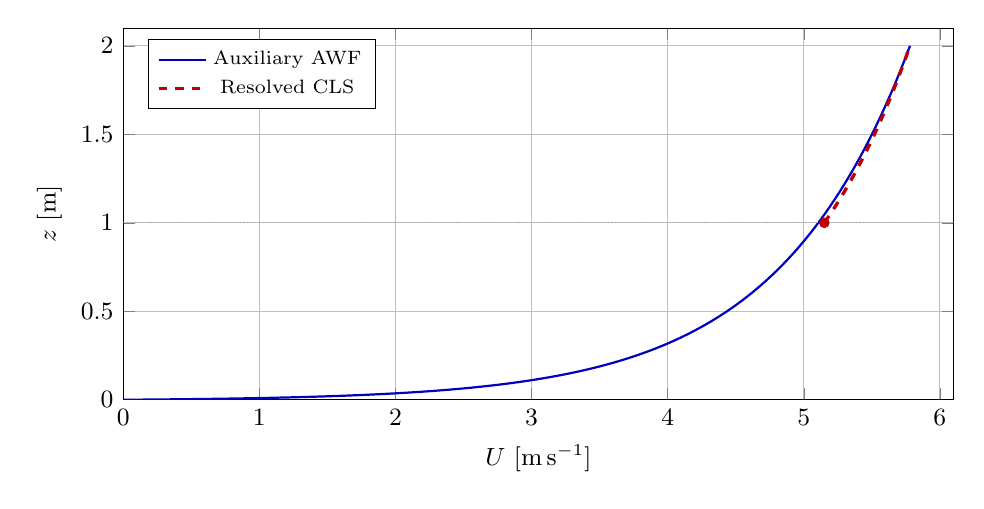
\begin{tikzpicture}
\begin{axis}[
width=\linewidth,height=6.3cm,
xlabel={$U\ [\mathrm{m\,s^{-1}}]$},
ylabel={$z\ [\mathrm m]$},
xmin=0,xmax=6.1,ymin=0,ymax=2.1,
grid=major,legend style={font=\scriptsize,at={(0.03,0.97)},anchor=north west},
tick label style={font=\small},label style={font=\small}]
\addplot[blue!75!black,thick,domain=0:5.780254368,samples=160]
 {0.0008795103205732289/0.16397739074295414*
 (exp(0.16397739074295414*x/0.16)-1)};
\addlegendentry{Auxiliary AWF}
\addplot[red!75!black,very thick,dashed,
domain=5.150912830:5.780254368,samples=70]
 {2*exp(0.44055390518665866/0.4*(x-5.780254367996082))};
\addlegendentry{Resolved CLS}
\addplot[only marks,mark=*,mark size=1.7pt,red!75!black]
 coordinates {(5.150912830,1)};
\addplot[black!35,densely dotted,forget plot]
 coordinates {(0,1) (6.1,1)};
\end{axis}
\end{tikzpicture}
\end{minipage}\hfill
\begin{minipage}[t]{0.49\linewidth}
\centering
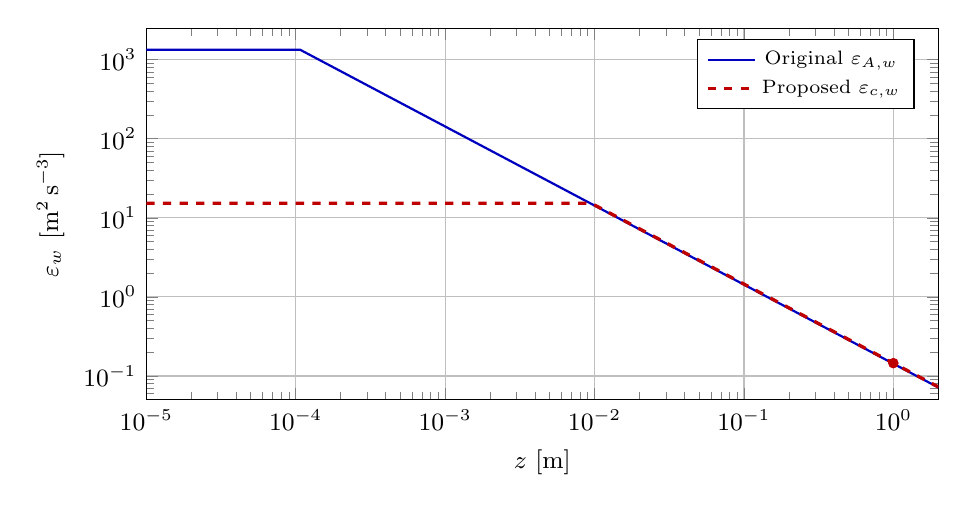
\begin{tikzpicture}
\begin{loglogaxis}[
width=0.96\linewidth,height=6.3cm,
xlabel={$z\ [\mathrm m]$},
ylabel={$\eps_w\ [\mathrm{m^2\,s^{-3}}]$},
xmin=1e-5,xmax=2,ymin=0.05,ymax=2500,
grid=major,legend style={font=\scriptsize,at={(0.97,0.97)},anchor=north east},
tick label style={font=\small},label style={font=\small}]
\addplot[blue!75!black,thick] coordinates {
 (1e-5,1335.990933735)
 (0.00010706811421,1335.990933735)
 (2,0.071521014939)};
\addlegendentry{Original $\eps_{A,w}$}
\addplot[red!75!black,very thick,dashed] coordinates {
 (1e-5,15.267215713)
 (0.00951526913991,15.267215713)
 (2,0.072635833262)};
\addlegendentry{Proposed $\eps_{c,w}$}
\addplot[only marks,mark=*,mark size=1.7pt,red!75!black]
 coordinates {(1,0.145271666524)};
\end{loglogaxis}
\end{tikzpicture}
\end{minipage}
\caption{Left: the auxiliary velocity satisfies $U_A(0)=0$ and matches
the outer reference at $H=2\units m$. The original CLS logarithm on $z\geq z_P$ is the FV comparison;
the marked point is its FV value at $P$. In the selected spectral/$hp$
construction the blue analytical reconstruction is the numerical velocity
throughout $0\leq z\leq H$, and the CLS branch begins at $H$. Right: the modified inner dissipation reduces the cell mean
while retaining the CLS tail at resolved heights. A wall-model
distribution and the resolved field have distinct roles.}
\label{fig:profiles}
\end{figure}

At frozen $U_n=U_{n,0}$ and $K=K_0$, the following forcing changes are
retained exactly by the proposed momentum and production operators:
\begin{table}[htbp]
\centering\small
\begin{tabular}{@{}rrr@{}}
\toprule
$F\ [\mathrm{m\,s^{-2}}]$ &
$t_A\ [\mathrm{m^2\,s^{-2}}]$ &
$\avg P_A\ [\mathrm{m^2\,s^{-3}}]$\\
\midrule
$-0.02$ & $0.1653666328$ & $0.4624825900$\\
$0$ & $0.1600000000$ & $0.4610926090$\\
$0.03$ & $0.1519500508$ & $0.4645406939$\\
\bottomrule
\end{tabular}
\caption{Unchanged finite forcing response at equal wall-law inputs.
The matching velocity remains $5.780254368\units{m\,s^{-1}}$
in all three integrations.}
\label{tab:pressure}
\end{table}
Independent double-precision quadrature gives the wall-cell source and
matching-velocity identities to better than $10^{-11}$ in the displayed
SI units. The molecular contribution to \cref{eq:energy} is
$0.002655480883\units{m^3\,s^{-3}}$, and the energy residual is below
$10^{-12}\units{m^3\,s^{-3}}$.
These checks test the scalar roots, tensor reduction, and wall identities.
They do not test a spatially discretized CFD solver.

\subsection{Higher-order source moments and the new redistribution}
For the same example, let $\mathcal L_j$ be the degree-$j$ Legendre
polynomial and test with $v_j(z)=\mathcal L_j(2z/H-1)$. The unweighted
height moments in \cref{tab:hp-moments} have units
$\mathrm{m^3\,s^{-3}}$ and are per unit density and wall area.
The original capped-profile source has a zero mean but nonzero higher
moments. They remain under accurate integration and would force a
constant-$k$ Galerkin field away from equilibrium.

\begin{table}[htbp]
\centering\small
\begin{tabular}{@{}crr@{}}
\toprule
$j$ & $\int_0^H v_j(p_{A,0}-\ECw)\,\dd z$
& $\int_0^H v_j S_{k,0}^{hp}\,\dd z$\\
\midrule
0 & $<2\times10^{-12}$ in magnitude & $0$ algebraically\\
1 & $ 1.73551439079\times10^{-2}$ & $0$ algebraically\\
2 & $-2.20336637626\times10^{-2}$ & $0$ algebraically\\
3 & $ 2.20527999939\times10^{-2}$ & $0$ algebraically\\
4 & $-1.97059614435\times10^{-2}$ & $0$ algebraically\\
5 & $ 1.60477076949\times10^{-2}$ & $0$ algebraically\\
6 & $-1.16765463336\times10^{-2}$ & $0$ algebraically\\
\bottomrule
\end{tabular}
\caption{Mean compatibility alone does not imply higher-mode compatibility.
The corrected source is evaluated in its simplified pointwise form;
the executable check requires each resulting load to be below
$2\times10^{-12}$ in the stated SI units.}
\label{tab:hp-moments}
\end{table}

The added verification evaluates $j_{\rm red}$ independently through
closed production and dissipation primitives, verifies its zero
endpoint values, and checks agreement between source moments and
integration-by-parts flux loads. It also verifies that the forcing
increments between $F=-0.02$ and $0.03\units{m\,s^{-2}}$ agree in
every tested mode for fixed $\chi=0,0.37,1$. The required tolerances
are $2\times10^{-12}$ for redistribution identities and
$3\times10^{-12}$ for the modal forcing increments. These checks
exercise the new model term rather than merely repeating its formula.

\subsection{Finite polynomial representation and interface stress}
On the fixed outer interval $[H,2H]$, interpolate the exact logarithm
at Gauss--Lobatto--Legendre nodes. The stored nodal values agree to
roundoff, while an independent set of interior evaluation points gives
the nonzero errors in \cref{tab:hp-projection}. This demonstrates why
the discrete target and full residual must be specified separately.

\begin{table}[htbp]
\centering\small
\begin{tabular}{@{}crr@{}}
\toprule
Degree $p_h$ & Maximum sampled velocity error
& Maximum sampled gradient error\\
& $\mathrm{m\,s^{-1}}$ & $\mathrm{s^{-1}}$\\
\midrule
2 & $5.45151\times10^{-3}$ & $3.18969\times10^{-2}$\\
4 & $8.76693\times10^{-5}$ & $1.28353\times10^{-3}$\\
8 & $4.08789\times10^{-8}$ & $1.42296\times10^{-6}$\\
\bottomrule
\end{tabular}
\caption{Interpolation checks at fixed matching height. These are sampled
errors on one outer element, not error bounds or Nektar++ solver results.}
\label{tab:hp-projection}
\end{table}

The appended code also checks the stress transfer
$T_H=t_A+F(H-h)$ and the scalar conormal sign in
\cref{eq:hp-robin-scalar}. In the numerical example,
$\partial t_A/\partial F=-0.2683316414\units m$, whereas
$\partial T_H/\partial F=1.6316683586\units m$.
Their difference is $H-h=1.9\units m$, the integrated forcing length.
The analytical ground velocity is checked independently at $z=0$.
These results do not establish the outer assembled residual, the
normal-velocity/pressure coupling in developing flow, or
\cref{eq:hp-time-fixedpoint}.


\subsection{Curved geometry and conservative flux checks}
\label{sec:curve-numerical}
Appendix~\ref{app:curve-stability-checks} adds an independent
manufactured-field check on an extruded circular hill segment. Its
curvature is $c=0.05\ \mathrm{m^{-1}}$, with
$\bm n'=c\bm t$, $\bm t'=-c\bm n$ and $J=1+cr$. Use
\begin{equation}
 \begin{gathered}
 a(s)=1+0.1\cos(0.4s),\qquad
 H(s)=2+0.2\sin(0.3s),\\
 u_t(s,r)=a(s)r,\qquad
 w(s,r)=-\frac{a'(s)r^2}{2(1+cr)}.
 \end{gathered}
 \label{eq:curve-test-field}
\end{equation}
Lengths are in metres; the coefficients of $a$ have units
$\mathrm{s^{-1}}$ and the trigonometric arguments are dimensionless.
This field is exactly incompressible, is zero at the ground, and
obeys the mapped gradient identity. At $s=1.3\ \mathrm m$,
\begin{equation}
 \begin{aligned}
 H&=2.0760376830\ \mathrm m,&
 w_H&=0.03880261243\ \mathrm{m\,s^{-1}},\\
 m_H&=-0.08237640447\ \mathrm{m\,s^{-1}},&
 J_Hw_H&=+0.04283039671\ \mathrm{m\,s^{-1}}.
 \end{aligned}
 \label{eq:curve-test-mass}
\end{equation}
Omitting the matching-height slope even reverses the inferred flux
direction in this example. Integrating over
$-3\leq s\leq2.5\ \mathrm m$ with an arbitrary constant Cartesian
stress, the closed-boundary momentum flux agrees with the volume
acceleration to $3.1\times10^{-15}$ in the numerical units. The
closed mass flux is zero to roundoff. A separate manufactured scalar
with variable diffusivity gives a flux/source mismatch of
$5.4\times10^{-15}$. These compare volume integrals with independently
formed top, ground, and lateral fluxes, and exercise the actual
sloped-interface normal.

For the same curvature, $u_t=r\ \mathrm{s^{-1}}$ and $w=0$ give a
curvature-only normal-pressure increment between $r=0$ and $2\ \mathrm m$
of
\begin{equation}
 \Delta(p/\rho)=\int_0^2\frac{cr^2}{1+cr}\,\dd r
 =0.12407192173\ \mathrm{m^2\,s^{-2}}.
 \label{eq:curve-test-pressure}
\end{equation}
Gravity can be added through its potential separately. This test
checks the normal-acceleration sign, not an AWF velocity prediction.
Using $J=1+cr$ in the original numerical wall example changes the
metric-balanced cutoff to $r_c=0.009458614009\ \mathrm m$; the
independent integral of $J(\ECw-p_{A,0})$ is
$2.3\times10^{-15}$ in numerical units. This is a redistribution
check, not a claim that a curved flow has the flat reference production.
The spatial gate is also checked for its exact unit and zero plateaus.

\subsection{Reproducible constitutive failure}
\label{sec:stability-numerical}
The additional script evaluates the complete stated CLS tensor,
compares its $c_4$ matrix form with an independent indexed contraction,
and checks both invariant branches. In the dimensionless normalization
$G=\eps=\nu_t=1$, $k=\qs$, the exact transverse flux block is
\begin{equation}
 \begin{pmatrix}
 -0.964557906564&-1.148643029385\\
  1.148643029385&1
 \end{pmatrix}.
 \label{eq:stability-test-block}
\end{equation}
Central finite differences of the \emph{full} nonlinear stress give
\begin{center}
\begin{tabular}{@{}cc@{}}
\toprule
Perturbation amplitude $g$ &
$-[R_{yx}(g)-R_{yx}(-g)]/(2g)$\\
\midrule
$10^{-3}$&$-0.964555919193$\\
$10^{-5}$&$-0.964557906365$\\
$10^{-7}$&$-0.964557906564$\\
\bottomrule
\end{tabular}
\end{center}
The perturbed covariance remains strictly positive and the first
production variation remains zero. These are independent checks of
\cref{eq:stability-negative-diffusion}, not evidence of stability.

As a supporting check away from the invariant tie, take a gradient
$L$ with $L_{xz}=1$, $L_{xx}=10^{-4}$, $L_{zz}=-10^{-4}$ and all
other entries zero. It has $\widetilde S>\widetilde\Omega$ and a
well-defined classical derivative. For
\begin{equation}
 \bm\xi=(0.45,0,\sqrt{1-0.45^2}),\qquad
 \bm a=(-\xi_z,0,0.45),
 \label{eq:stability-inplane-direction}
\end{equation}
the incompressible form in \cref{eq:stability-symbol} is
$-0.02596757790$ in the same normalization. Thus even a nearby
two-dimensional strain-dominant state has an adverse principal
direction. The script's final message distinguishes successful
identity checks from the failed constitutive-stability criterion.
No time integration, pressure solve, assembled Nektar++ residual,
or long-time terrain simulation is performed by either appendix.


\section{Limits, interpretation, and next validation steps}
\label{sec:limits}
\subsection{Finite Reynolds number terms}
The outer solution is exact for the stated high Reynolds number
equations, not for the full low Reynolds number CLS equations at every
height. On the candidate reference,
\begin{equation}
 R_t(z)=\frac{\qs^2\kc\ust z}{\nu},\qquad
 \nu_{t,0}^{\rm full}=f_\mu(R_t)\kc\ust z.
\label{eq:Rtref}
\end{equation}
The corresponding total stress in the full molecular-plus-turbulent
momentum equation would be
\begin{equation}
 (\nu+\nu_{t,0}^{\rm full})U_0'
 =\frac{\nu\ust}{\kc z}+f_\mu(R_t)\ust^2,
\label{eq:finiteRestress}
\end{equation}
which is not exactly constant. Molecular dissipation diffusion and the
other finite Reynolds number terms can also leave residuals.
Retaining $\nu$ in the AWF integration does not remove these bulk
residuals. One must either use the stated outer approximation where it
is appropriate, or compute a different reference for the complete
finite Reynolds number equations.

\subsection{Model attribution and intended use}
The algebraic Yap term used in \cref{eq:Yap} is the original CLS
length-scale correction. The AWF paper's later sand-dune calculations
also discuss a \emph{differential} length-scale correction
\cite[discussion of Fig.~14]{SCI2006}. That later variant is not
silently substituted into this note; changing the resolved turbulence
equations requires a new equilibrium derivation.

The capped reference dissipation, source redistribution, physical
transition, mapped patch completion, roughness-force bookkeeping,
and condensation/interface choices are proposed here. They are not
attributed to the original papers. Their baseline is now defined at
the operator level in \cref{sec:transition}. The normal-tube equations
are a complete mathematical specification, subject to their stated
boundary data and model assumptions; they are not physical validation
over unresolved roughness or proof of a curved equilibrium.

\begin{table}[htbp]
\centering\small
\begin{tabularx}{\linewidth}{@{}p{0.30\linewidth}X@{}}
\toprule
Result or requirement & Status in this revision\\
\midrule
Outer neutral reference & Derived for the selected constant-$k$,
high-Re branch with the original algebraic Yap term\\
FV and modal budgets & FV mean balance retained; additional signed
redistribution cancels all flat-reference wall source moments\\
Ground no slip & Exact for the flat analytical reconstruction;
essential condition of the curved patch solve\\
Curved geometry and transport & Derived mapped momentum, continuity,
$k$/outer-$\eps$ transport, admissibility and variable-$H$ fluxes\\
Pressure and interface coupling & Full traction and common mass/$k$
flux; independent pressure spaces admit the required normal-stress offset\\
Inner dissipation & Dependent profile and one outer value trace;
no claimed globally solved dissipation conservation law\\
Spatial transition/baseline & Fixed upstream fade; $\chi=0$ through
hill/wake; same curved operator with original-form dissipation and $C_k^w=0$\\
Discrete anchor & Optional global flat verification only;
$\eta=0$ throughout the selected hill calculation\\
Constitutive stability & \textbf{Failed} for the stated unchanged
high-Re CLS law: an exact transverse direction has negative diffusion\\
Inner turbulence positivity & \textbf{Not generally preserved} by a
sampled sink acting on a transported wall-normal $k$ field\\
Executable checks & Scalar/modal identities, curved volume/flux
budgets, metric cutoff and constitutive counterexample reproduced\\
Nektar++ and long-time qualification & Integration contract supplied;
no native implementation or long-time CFD evidence claimed\\
\bottomrule
\end{tabularx}
\caption{Mathematical results, demonstrated obstructions, and remaining qualification.}
\label{tab:status}
\end{table}

For a robust implementation, first declare how the constitutive and
positivity obstructions are addressed and whether that changes the
adapted baseline. Then qualify the actual curved patch coupling and
all-field residual, pressure stages, and time map. A regularization
that preserves the value of the flat reference may still change its
perturbation dynamics and terrain response. Neither successful local
quadrature nor steady solver convergence can replace those tests.
The original analytical forcing response is retained in its specified
flat reduction; separation and reattachment over terrain are
predictions of the newly completed coupled operator and require
independent validation.

\appendix
\section{Closed AWF integrals}
\label{app:integrals}
\subsection{Viscosity segments and momentum integrals}
Define
\begin{equation}
 z_v=\frac{\nu b}{\sqrt K},\quad
 a_A=\alpha\sqrt K,\quad d_A=\nu-a_Az_v,\quad
 z_s=\min[H,\max(0,z_v)].
\label{eq:segments}
\end{equation}
The molecular segment is $0\leq z<z_s$ when $z_s>0$; the
turbulent segment, if present, has $D_A=d_A+a_Az$.
If $H>z_s$, set $D_s=d_A+a_Az_s$ and $D_H=d_A+a_AH$.
Then
\begin{align}
 J_0&=\frac{z_s}{\nu}+\frac1{a_A}\ln\frac{D_H}{D_s},\\
 J_2&=\frac{z_s}{\nu^2}
       +\frac1{a_A}\left(\frac1{D_s}-\frac1{D_H}\right).
\label{eq:Jclosed}
\end{align}
If $H=z_s$, the layer is entirely molecular and
$J_0=H/\nu$, $J_2=H/\nu^2$, $P_0=0$. Such a layer fails
\cref{eq:gate} for a positive CLS reference.

For $0\leq h<H$, the molecular contribution to $J_1$ is
\begin{equation}
 J_{1,m}=\frac{\pos{z_s-h}^2}{2\nu}.
\end{equation}
Set $\ell=\max(h,z_s)$. If $\ell<H$, the turbulent contribution is
\begin{equation}
 J_{1,t}=\frac{H-\ell}{a_A}
 -\frac{d_A+a_Ah}{a_A^2}
       \ln\frac{d_A+a_AH}{d_A+a_A\ell};
\label{eq:J1closed}
\end{equation}
otherwise it is zero. Thus $J_1=J_{1,m}+J_{1,t}$.
The same expressions with an upper limit $z\leq H$ evaluate
$J_0(z)$ and $J_1(z)$, after recomputing the segment limits.
In particular, $J_1(z)=0$ when $z\leq h$.

\subsection{Production primitive}
On a turbulent segment whose stress is affine,
write $T(z)=t_b+g_bz$ and $w=d_A+a_Az$. Put
\begin{equation}
 \lambda=\frac{g_b}{a_A},\qquad
 \delta=t_b-\frac{g_bd_A}{a_A},\qquad T=\lambda w+\delta.
\end{equation}
An antiderivative is
\begin{align}
 \int\frac{\nu_{t,A}T^2}{D_A^2}\,\dd z
 =\frac1{a_A}\bigg[
 &\frac{\lambda^2w^2}{2}
 +(2\lambda\delta-\nu\lambda^2)w
\nonumber\\
 &+(\delta^2-2\nu\lambda\delta)\ln\frac w\nu
 +\frac{\nu\delta^2}{w}\bigg].
\label{eq:Pprimitive}
\end{align}
For $z<h$, use $(t_b,g_b)=(t_A,0)$; for $z>h$,
use $(t_b,g_b)=(t_A-Fh,F)$. Sum endpoint differences over
the turbulent segments, splitting at $h$ when necessary, and divide
by $H$ to obtain $\avg P_A$. The molecular segments contribute zero
turbulent production. In the vector form, replace $\lambda^2$ and
$\delta^2$ by squared norms and $\lambda\delta$ by the dot product.

Closed forms are useful in a solver, while quadrature with explicit
breakpoints provides an independent verification and avoids cancellation
in marginally turbulent cases. Stable evaluation of logarithmic ratios,
for example with \texttt{log1p} when appropriate, is advisable.
\section{Executable numerical verification}
\label{app:verification}
The following self-contained Python code requires Python~3, NumPy, and
SciPy. Copy the listing into a \texttt{.py} file and run it to reproduce
the scalar constants and example. It checks the uncontracted tensor
reduction in normalized simple shear, the positive covariance, the
integrated dissipation and energy identities, and finite forcing
increments. All dimensional inputs and outputs use SI units.
Explicit quadrature breakpoints are used at the viscosity, roughness,
and dissipation transitions. This is an algebraic and quadrature
verification, not a CFD stability or terrain-validation test. The
added part checks modal source moments, redistribution by integration
by parts, matching-surface stress, and fixed-height polynomial
interpolation. It does not invoke Nektar++ or test its assembled solver.

\begin{lstlisting}[style=py]
import math
import numpy as np
from scipy.integrate import quad
from scipy.optimize import brentq

def C(q):
    return (0.3 / (1 + 0.35*q**1.5)
            * -math.expm1(-0.36*math.exp(0.75*q)))

def HY(r):
    return 0.83*max(r-1, 0)*r*r

q = brentq(lambda x: C(x)*x*x-1, 1, 8, xtol=5e-15)
kap = brentq(
    lambda x: q*x*x/1.3 + HY(x*q**1.5/2.5)-0.48,
    0.3, 0.6, xtol=5e-15)
assert abs(C(q)*q*q-1) < 1e-13
assert abs(q*kap*kap/1.3 + HY(kap*q**1.5/2.5)-0.48) < 1e-13

# Full tensor evaluation in Cartesian order (x, y, z).
# Normalization: G=1, ustar=1, k=q, epsilon=nut=1.
S = np.array([[0., 0., 1.], [0., 0., 0.], [1., 0., 0.]])
O = np.array([[0., 0., 1.], [0., 0., 0.], [-1., 0., 0.]])
I = np.eye(3)
SS, OO = np.sum(S*S), np.sum(O*O)
c1, c2, c3 = -0.1, 0.1, 0.26
c4, c5, c6, c7 = -10*C(q)**2, 0., -5*C(q)**2, 5*C(q)**2
T4 = (np.einsum("ki,lj,kl->ij", S, O, S)
      + np.einsum("kj,li,kl->ij", S, O, S))
T5 = O@O@S + S@O@O - (2/3)*np.trace(S@O@O)*I
anis = (-S/q + c1*(S@S.T-SS*I/3)
        + c2*(O@S.T+S@O.T) + c3*(O@O.T-OO*I/3)
        + q*(c4*T4+c5*T5+(c6*SS+c7*OO)*S))
RbyK = (2/3)*I + anis
expected = np.array([[.92, 0, -1/q], [0, .56, 0], [-1/q, 0, .52]])
assert np.max(np.abs(RbyK-expected)) < 1e-13
assert min(np.linalg.eigvalsh(RbyK)) > 0

# Illustrative rough-wall case; continuum matching at H.
ustar, nu, h, H, zP = 0.4, 1.5e-5, 0.1, 2., 1.
K0 = q*ustar*ustar
K, t0 = K0, ustar*ustar
cmu_w, cl_w, zvs_star = 0.09, 2.55, 10.7
alpha, ze_star = cmu_w*cl_w, 2*cl_w
sqK = math.sqrt(K)
xs = h*sqK/(70*nu)
m = max(0.5-0.4*xs**0.7, 1-0.79*xs**(-0.28))
b = zvs_star*(1-xs**m)

def nut(z):
    return nu*max(0, alpha*(z*sqK/nu-b))

def D(z):
    return nu+nut(z)

def Lh(z):
    return max(z-h, 0)

def Q(fun, end=H, extra=()):
    pts = sorted({p for p in (h, b*nu/sqK, *extra) if 0 < p < end})
    return quad(fun, 0, end, points=pts,
                epsabs=1e-12, epsrel=2e-13)[0]

J0 = Q(lambda z: 1/D(z))
J1 = Q(lambda z: Lh(z)/D(z))
J2 = Q(lambda z: 1/D(z)**2)
B, Un0, Ac = J1/J0, t0*J0, ustar**3/kap
P0 = t0*t0/H * Q(lambda z: nut(z)/D(z)**2)
Lam = H*P0/Ac
zc = H*math.exp(1-Lam)
z0 = H*math.exp(-kap*Un0/ustar)
zeA = ze_star*nu/sqK
assert Lam >= 1+math.log(H/zP)
assert 0 < zc <= zP < H

def eA(z):
    return 2*nu*K/zeA**2 if z < zeA else K**1.5/(cl_w*z)

def eC(z):
    return Ac/max(z, zc)

def tau(F):
    return Un0/J0-B*F

def grad(z, F):
    return (tau(F)+F*Lh(z))/D(z)

eAmean = K**1.5/(cl_w*H)*(1+math.log(H/zeA))
eCmean = Q(eC, extra=(zc,))/H
molecular_power = nu*Q(lambda z: grad(z, 0)**2)
energy_residual = t0*Un0-H*eCmean-molecular_power
assert abs(Q(eA, extra=(zeA,))/H-eAmean) < 2e-12
assert abs(2*nu*K/zeA**2-K**1.5/(cl_w*zeA)) < 2e-12
assert abs(P0-eCmean) < 2e-12
assert abs(eC(zP)-Ac/zP) < 2e-12
assert abs(energy_residual) < 2e-12
assert abs(P0-t0*t0/H*(J0-nu*J2)) < 2e-12
assert abs(zc-math.e*z0*math.exp(kap*ustar*nu*J2)) < 2e-12

Lj = [Q(lambda z, j=j: nut(z)/D(z)**2*(Lh(z)-B)**j)/H
      for j in range(3)]
for F in (-0.02, 0., 0.03):
    PF = Q(lambda z: nut(z)*grad(z, F)**2)/H
    PP = Lj[0]*t0*t0 + 2*Lj[1]*t0*F + Lj[2]*F*F
    assert abs(PF-PP) < 2e-12
    assert abs(Q(lambda z: grad(z, F))-Un0) < 2e-11
    print("F, traction/rho, production:", F, tau(F), PF)
assert abs(tau(.03)-tau(-.02)+B*.05) < 2e-12

values = dict(q=q, Cmu=C(q), kappa=kap, Yap=HY(kap*q**1.5/2.5),
              K0=K0, K=K, ustar=ustar, J0=J0, J1=J1, B=B, Un0=Un0,
              UP_CLS=Un0+ustar/kap*math.log(zP/H),
              UP_AWF=t0*Q(lambda z: 1/D(z), end=zP),
              Ac=Ac, P0=P0, eAmean=eAmean, eCmean=eCmean,
              eA_P=eA(zP), eC_P=eC(zP), zc=zc, z0=z0,
              Lambda=Lam, energy_residual=energy_residual)
for name, value in values.items():
    print(f"{name:16s} {value:.15g}")
print("Covariance eigenvalues:", np.linalg.eigvalsh(RbyK))
print("All algebraic and quadrature checks passed.")
# Append after the original note's verification listing.
# This is a local analytical/quadrature check, not a Nektar++ run.
from scipy.special import eval_legendre
from scipy.interpolate import BarycentricInterpolator
from numpy.polynomial.legendre import Legendre

def PAref(z):
    return nut(z)*grad(z, 0.0)**2

def Ck(z):
    # New signed redistribution, not an additional dissipation field.
    return eC(z)-PAref(z)

def moment(j, fun):
    return Q(lambda z: eval_legendre(j, 2*z/H-1)*fun(z),
             extra=(zc, zeA))

def source_old(z, F, chi=1.0):
    return (nut(z)*grad(z, F)**2
            -(1-chi)*eA(z)-chi*eC(z))

def source_new(z, F, chi=1.0):
    # Algebraically: source_old + chi*Ck.
    # This form avoids cancellation of two large copies of eC.
    return (nut(z)*grad(z, F)**2
            -(1-chi)*eA(z)-chi*PAref(z))

# Independent closed primitive of reference production, with the
# molecular segment contributing no turbulent production.
def production_primitive(z):
    a = alpha*sqK
    zv = b*nu/sqK
    lower = max(0.0, zv)
    if z <= lower:
        return 0.0
    d = nu-a*zv
    Dl, Dz = d+a*lower, d+a*z
    delta = a*(z-lower)
    return t0*t0/a*(math.log1p(delta/Dl)-nu*delta/(Dl*Dz))

def dissipation_primitive(z):
    if z <= zc:
        return Ac*z/zc
    return Ac*(1+math.log(z/zc))

def jred(z):
    # Gradient-flux convention: +d(jred)/dz is added to the k RHS.
    return dissipation_primitive(z)-production_primitive(z)

assert abs(jred(0.0)) < 2e-12
assert abs(jred(H)) < 2e-12
assert abs(Q(Ck, extra=(zc,))) < 2e-12

for j in range(7):
    old = moment(j, lambda z: source_old(z, 0.0))
    new = moment(j, lambda z: source_new(z, 0.0))
    load = moment(j, Ck)
    dtest = Legendre.basis(j).deriv()
    # Integration by parts checks the independently formed primitive.
    flux_load = (eval_legendre(j, 1.0)*jred(H)
                 -eval_legendre(j, -1.0)*jred(0.0)
                 -Q(lambda z: (2/H)*dtest(2*z/H-1)*jred(z),
                    extra=(zc,)))
    assert abs(new) < 2e-12
    assert abs(old+load) < 2e-12
    assert abs(load-flux_load) < 2e-12
    if j > 0:
        assert abs(old) > 1e-5
    print('mode, old k load, corrected k load:', j, old, new)

# At frozen K, matching velocity, and chi, all production forcing
# increments are retained, including the higher Galerkin moments.
F1, F2 = -0.02, 0.03
max_forcing_error = 0.0
for chi in (0.0, 0.37, 1.0):
    for j in range(7):
        original_increment = moment(
            j, lambda z: source_old(z, F2, chi)
                         -source_old(z, F1, chi))
        new_increment = moment(
            j, lambda z: source_new(z, F2, chi)
                         -source_new(z, F1, chi))
        err = abs(new_increment-original_increment)
        max_forcing_error = max(max_forcing_error, err)
        assert err < 3e-12
print('max modal frozen-forcing error:', max_forcing_error)
print('redistribution primitive at 0,H:', jred(0.0), jred(H))

# A finite polynomial can interpolate the exact logarithm at every
# stored GLL node without reproducing its off-node values or derivative.
# Use an OUTER element [H,2H], where the reference is nonsingular.
sample_z = H*(1+(np.arange(257)+0.5)/257)
for pdeg in (2, 4, 8):
    gll = np.r_[-1.0, Legendre.basis(pdeg).deriv().roots(), 1.0]
    nodes_z = H*(1.5+0.5*gll)
    exact_nodes = Un0+ustar/kap*np.log(nodes_z/H)
    poly = BarycentricInterpolator(nodes_z, exact_nodes)
    exact_sample = Un0+ustar/kap*np.log(sample_z/H)
    value_error = np.max(np.abs(poly(sample_z)-exact_sample))
    gradient_error = np.max(np.abs(poly.derivative(sample_z)
                                    -ustar/(kap*sample_z)))
    assert np.max(np.abs(poly(nodes_z)-exact_nodes)) < 2e-13
    assert value_error > 1e-12
    assert gradient_error > 1e-11
    print('p, off-node velocity error, gradient error:',
          pdeg, value_error, gradient_error)
print('All added local hp checks passed; no solver gate is inferred.')

# Interface traction is distinct from the physical wall traction.
for F in (-0.02, 0.0, 0.03):
    TH = tau(F) + F*(H-h)
    assert abs(TH - Un0/J0 - F*((H-h)-B)) < 2e-13
    # Scalar conormal Robin balance, outward normal -e_z.
    assert abs(-TH + Un0/J0 - F*(B-(H-h))) < 2e-13
assert abs((tau(.03)+.03*(H-h))-(tau(-.02)-.02*(H-h))
           -((H-h)-B)*.05) < 2e-13
assert abs(t0*Q(lambda z: 1/D(z), end=0.0)) < 2e-13
print("Interface stress and reconstructed no-slip checks passed.")

\end{lstlisting}

\section{Executable curved-geometry and constitutive checks}
\label{app:curve-stability-checks}
This second standalone Python listing requires NumPy and SciPy.
It checks the manufactured curved field and independent boundary/volume
fluxes, a metric-weighted cutoff, switch plateaus, the indexed cubic
tensor, and finite-difference stress tangents. Its constitutive result
is a verified failure of the necessary stability condition. It does
not run Nektar++ or perform a temporal CFD experiment. The geometry
tests use a finite circular segment with an admissible normal map;
they do not certify the geometry of an unspecified production hill.

\begin{lstlisting}[style=py]
"""Geometry, flux, switch and constitutive checks; no CFD time solve.
Run with Python 3, NumPy and SciPy. All tensors use (x,y,z).
"""
import numpy as np
from scipy.integrate import quad
from scipy.optimize import brentq
from numpy.polynomial.legendre import leggauss


def integrate(fun, lo, hi, count=48):
    x, w = leggauss(count)
    return sum(wi * fun(lo + (hi-lo)*(xi+1)/2)
               for xi, wi in zip(x, w)) * (hi-lo)/2


# A circular hill segment: X'(s)=t, n'(s)=curv*t.
curv = 0.05
T = np.array([[0.7, 0.1, -0.2], [0.1, -0.3, 0.05],
              [-0.2, 0.05, 1.1]])  # constant Cartesian stress


def geometry(s, r):
    t = np.array([np.cos(curv*s), 0., -np.sin(curv*s)])
    n = np.array([np.sin(curv*s), 0., np.cos(curv*s)])
    J = 1 + curv*r
    A = 1 + 0.1*np.cos(0.4*s)
    Ap = -0.04*np.sin(0.4*s)
    App = -0.016*np.cos(0.4*s)
    u = A*r
    w = -Ap*r*r/(2*J)
    us, ur = Ap*r, A
    ws = -App*r*r/(2*J)
    wr = -Ap*r*(2+curv*r)/(2*J*J)
    U = u*t+w*n
    grad = (np.outer(((us+curv*w)*t+(ws-curv*u)*n)/J, t)
            + np.outer(ur*t+wr*n, n))
    return J, t, n, U, grad


def height(s):
    return 2+0.2*np.sin(0.3*s), 0.06*np.cos(0.3*s)


def scalar(s, r):
    k = 2+0.1*np.sin(s)+0.2*r*r
    ks, kss, kr, krr = 0.1*np.cos(s), -0.1*np.sin(s), 0.4*r, 0.4
    D, Dp = 1+0.1*r, 0.1
    J, t, n, U, grad = geometry(s, r)
    gradk = t*ks/J+n*kr
    diffusion = D*krr+(Dp+curv*D/J)*kr+D*kss/J**2
    source = U@gradk-diffusion
    return k, U*k-D*gradk, source


# Independent Cartesian differentiation of the manufactured velocity.
for s in (-2., 0.7, 2.1):
    for r in (0.1, 0.8, 1.7):
        J, t, n, U, grad = geometry(s, r)
        hfd = 2e-5
        Us = (geometry(s+hfd, r)[3]-geometry(s-hfd, r)[3])/(2*hfd)
        Ur = (geometry(s, r+hfd)[3]-geometry(s, r-hfd)[3])/(2*hfd)
        grad_fd = np.outer(Us/J, t)+np.outer(Ur, n)
        assert np.max(np.abs(grad-grad_fd)) < 2e-10
        assert abs(np.trace(grad)) < 3e-16


def upper_flux(s, which):
    H, Hp = height(s)
    J, t, n, U, grad = geometry(s, H)
    area_normal = J*n-Hp*t  # N_H dS_H/ds
    if which == 'mass':
        return U@area_normal
    if which == 'momentum':
        return (np.outer(U, U)-T)@area_normal
    return scalar(s, H)[1]@area_normal


left, right = -3., 2.5
mass = integrate(lambda s: upper_flux(s, 'mass'), left, right)
mom = integrate(lambda s: upper_flux(s, 'momentum'), left, right)
mom += integrate(lambda s: T@geometry(s, 0)[2], left, right)
kflux = integrate(lambda s: upper_flux(s, 'k'), left, right)
for sign, s in ((-1, left), (1, right)):
    H, _ = height(s)
    mass += sign*integrate(lambda r: geometry(s, r)[3]@geometry(s, r)[1], 0, H)
    mom += sign*integrate(lambda r: (np.outer(geometry(s, r)[3],
           geometry(s, r)[3])-T)@geometry(s, r)[1], 0, H)
    kflux += sign*integrate(lambda r: scalar(s, r)[1]@geometry(s, r)[1], 0, H)
momvol = integrate(lambda s: integrate(lambda r:
    geometry(s, r)[0]*(geometry(s, r)[4]@geometry(s, r)[3]),
    0, height(s)[0]), left, right)
kvol = integrate(lambda s: integrate(lambda r:
    geometry(s, r)[0]*scalar(s, r)[2], 0, height(s)[0]), left, right)
assert abs(mass) < 2e-12
assert np.max(np.abs(mom-momvol)) < 2e-12
assert abs(kflux-kvol) < 2e-12
s = 1.3
H, Hp = height(s)
J, t, n, U, _ = geometry(s, H)
m = upper_flux(s, 'mass')
incorrect_m = J*(U@n)
assert m < 0 < incorrect_m  # ignoring H' even reverses its sign
print('curved balances:', mass, np.max(np.abs(mom-momvol)), kflux-kvol)
print('variable-H mass flux, correct / without slope:', m, incorrect_m)
dp = quad(lambda r: curv*r*r/(1+curv*r), 0, 2)[0]
assert abs(dp-(2-2/curv+np.log1p(2*curv)/curv**2)) < 1e-13
print('curvature pressure increment:', dp)


# A metric-weighted cutoff, using the physical AWF example.
qstar = 3.190675081624288
Cstar = 0.0982278953282113
kappa = 0.440553905186659
nu, ustar, rough, H = 1.5e-5, 0.4, 0.1, 2.0
K, alpha = qstar*ustar**2, 0.2295
hs = rough*np.sqrt(K)/nu
power = max(0.5-0.4*(hs/70)**0.7, 1-0.79*(hs/70)**(-0.28))
b = 10.7*(1-(hs/70)**power)
Ac = ustar**3/kappa


def nt(r):
    return nu*max(0., alpha*(r*np.sqrt(K)/nu-b))


def p0(r):
    return ustar**4*nt(r)/(nu+nt(r))**2


Pj = quad(lambda r: (1+curv*r)*p0(r), 0, H,
          epsabs=1e-12, epsrel=2e-12)[0]


def mean_cap(rc):
    return Ac*(1+np.log(H/rc)+curv*H-curv*rc/2)


rc = np.exp(brentq(lambda logrc: mean_cap(np.exp(logrc))-Pj,
                   np.log(H)-50, np.log(H), xtol=1e-13))
redistribution = (quad(lambda r: (1+curv*r)*(Ac/max(r, rc)-p0(r)),
                       0, rc, epsabs=1e-12)[0]
                  + quad(lambda r: (1+curv*r)*(Ac/max(r, rc)-p0(r)),
                         rc, H, epsabs=1e-12)[0])
assert abs(redistribution) < 2e-12
assert rc < 1.0
print('metric cutoff and redistribution integral:', rc, redistribution)


def gate(x):
    if x <= 0:
        return 1.0
    if x >= 1:
        return 0.0
    return 1-10*x**3+15*x**4-6*x**5


assert gate(-1) == 1 and gate(1) == 0 and gate(2) == 0
assert all(0 <= gate(x) <= 1 for x in np.linspace(-1, 2, 301))
assert abs(gate(0.5)-0.5) < 1e-15
print('spatial mask at normalized locations -1,0,0.5,1,2:',
      [gate(x) for x in (-1, 0, 0.5, 1, 2)])


# Exactly the note's high-Re CLS law, with an optional branch only
# for a smooth-branch derivative check. No coefficient is retuned.
def C(q):
    return 0.3/(1+0.35*q**1.5)*(-np.expm1(-0.36*np.exp(0.75*q)))


qs = brentq(lambda q: C(q)*q*q-1, 1, 8, xtol=5e-15)


def reynolds(L, branch='auto'):
    S, O = L+L.T, L-L.T
    ss, oo = np.sum(S*S), np.sum(O*O)
    qS, qO = qs*np.sqrt(ss/2), qs*np.sqrt(oo/2)
    q = qS if branch == 'S' else qO if branch == 'O' else (
        qS if np.real(qS) >= np.real(qO) else qO)
    c = C(q)
    nt = c*qs*qs
    I = np.eye(3)
    a = -nt/qs*S + nt*(-.1*(S@S-ss*I/3)
        + .1*(O@S-S@O) + .26*(O@O.T-oo*I/3))
    a += nt*qs*(-10*c*c*(S@S@O-O@S@S)
               + 5*c*c*(oo-ss)*S)
    return qs*(2*I/3+a)


L0 = np.zeros((3, 3)); L0[0, 2] = 1.
a, b = 1-20*C(qs), .36*qs
expected = np.array([[a, -b], [b, 1.]])
R0 = reynolds(L0)
assert np.linalg.eigvalsh(R0).min() > 1.
assert abs(-np.sum(R0*L0)-1) < 3e-14
rng = np.random.default_rng(83)
for _ in range(5):
    L = rng.normal(size=(3, 3))
    S, O = L+L.T, L-L.T
    indexed = (np.einsum('ki,lj,kl->ij', S, O, S)
               + np.einsum('kj,li,kl->ij', S, O, S))
    assert np.max(np.abs(indexed-(S@S@O-O@S@S))) < 1e-13
for branch in ('S', 'O'):
    block = np.zeros((2, 2))
    for j, column in enumerate((0, 2)):
        L = L0.astype(complex); L[1, column] += 1j*1e-30
        block[:, j] = -np.imag(reynolds(L, branch)[1, [0, 2]])/1e-30
    assert np.max(np.abs(block-expected)) < 3e-14
for amplitude in (1e-3, 1e-4, 1e-5, 1e-6, 1e-7):
    Lp, Lm = L0.copy(), L0.copy()
    Lp[1, 0], Lm[1, 0] = amplitude, -amplitude
    Rp, Rm = reynolds(Lp), reynolds(Lm)
    fd = -(Rp[1, 0]-Rm[1, 0])/(2*amplitude)
    dP = (-np.sum(Rp*Lp)+np.sum(Rm*Lm))/(2*amplitude)
    assert abs(fd-a) < 3*amplitude**2+2e-13
    assert abs(dP) < 2e-12
    assert np.linalg.eigvalsh(Rp).min() > 1.
    print('transverse finite difference:', amplitude, fd)
print('reference normalized covariance eigenvalues:', np.linalg.eigvalsh(R0/qs))
print('exact transverse flux block:', expected.tolist())

# Nearby strain-dominant state: differentiable actual max branch.
Ls = L0.copy(); Ls[0, 0] = 1e-4; Ls[2, 2] = -1e-4
xi = np.array([.45, 0., np.sqrt(1-.45**2)])
pol = np.array([-xi[2], 0., xi[0]])
dL = np.outer(pol, xi)
dT = -np.imag(reynolds(Ls.astype(complex)+1j*1e-30*dL))/1e-30
form = np.sum(dL*dT)
assert form < -.02
print('nearby smooth in-plane principal form:', form)
print('reference pressure jump / rho:', (0.52-2/3)*K)
print('PASS: identities verified; unchanged CLS stability gate FAILS.')

\end{lstlisting}

\begin{thebibliography}{99}
\bibitem{CLS1996}
T.~J. Craft, B.~E. Launder, and K. Suga,
Development and application of a cubic eddy-viscosity model of turbulence,
\emph{International Journal of Heat and Fluid Flow}
\textbf{17}(2), 108--115 (1996).
\href{https://doi.org/10.1016/0142-727X(95)00079-6}
{doi:10.1016/0142-727X(95)00079-6}.

\bibitem{SCI2006}
K. Suga, T.~J. Craft, and H. Iacovides,
An analytical wall-function for turbulent flows and heat transfer over
rough walls,
\emph{International Journal of Heat and Fluid Flow}
\textbf{27}(5), 852--866 (2006).
\href{https://doi.org/10.1016/j.ijheatfluidflow.2006.03.011}
{doi:10.1016/j.ijheatfluidflow.2006.03.011}.

\bibitem{MoninObukhov1954}
A.~S. Monin and A.~M. Obukhov,
Basic laws of turbulent mixing in the surface layer of the atmosphere,
\emph{Trudy Geofizicheskogo Instituta, Akademiya Nauk SSSR}
\textbf{24}(151), 163--187 (1954).
\href{https://www2.mmm.ucar.edu/wrf/users/physics/phys_refs/SURFACE_LAYER/eta_part1.pdf}
{English translation hosted by NCAR}.

\bibitem{RichardsHoxey1993}
P.~J. Richards and R.~P. Hoxey,
Appropriate boundary conditions for computational wind engineering models
using the $k$--$\eps$ turbulence model,
\emph{Journal of Wind Engineering and Industrial Aerodynamics}
\textbf{46--47}, 145--153 (1993).
\href{https://doi.org/10.1016/0167-6105(93)90124-7}
{doi:10.1016/0167-6105(93)90124-7}.

\bibitem{RichardsNorris2011}
P.~J. Richards and S.~E. Norris,
Appropriate boundary conditions for computational wind engineering models
revisited,
\emph{Journal of Wind Engineering and Industrial Aerodynamics}
\textbf{99}(4), 257--266 (2011).
\href{https://doi.org/10.1016/j.jweia.2010.12.008}
{doi:10.1016/j.jweia.2010.12.008}.
\bibitem{Brill2024}
S.~R. Brill, P. Pal, M. Ameen, C. Xu, and M. Ihme,
\emph{A Spectral Element Enrichment Wall-Model},
arXiv:2403.05670v3 (2024).
\url{https://arxiv.org/abs/2403.05670}.
This reference supports the enrichment strategy, not an implementation
of the present rough-wall CLS--AWF proposal.

\bibitem{NektarSpaces}
Nektar++ developers,
\emph{User Guide, version 5.10.0, Section 11.3:
Setting up the Simulation}.
\href{https://doc.nektar.info/userguide/5.10.0/user-guidese48.html}
{Official versioned user guide}.
Accessed 1 November 2026.

\bibitem{NektarExpansions}
Nektar++ developers,
\emph{User Guide, version 5.10.0, Section 3.2: Expansions}.
\href{https://doc.nektar.info/userguide/5.10.0/user-guidese7.html}
{Official versioned user guide}.
Accessed 1 November 2026.

\bibitem{NektarTheory}
Nektar++ developers,
\emph{Developer Guide, version 5.10.0, Section 14.1:
Fundamental Theories of IncNavierStokesSolver}.
\href{https://doc.nektar.info/developerguide/5.10.0/developer-guidese49.html}
{Official versioned developer guide}.
Accessed 1 November 2026.

\bibitem{NektarConditions}
Nektar++ developers,
\emph{Conditions.cpp, version 5.10.0 source documentation}.
\href{https://doc.nektar.info/doxygen/5.10.0/_conditions_8cpp_source.html}
{Official versioned source documentation}.
Accessed 1 November 2026.

\bibitem{NektarExpList}
Nektar++ developers,
\emph{ExpList.h, version 5.10.0 source documentation}.
\href{https://doc.nektar.info/doxygen/5.10.0/_exp_list_8h_source.html}
{Official versioned source documentation}.
Accessed 1 November 2026.

\bibitem{NektarContField}
Nektar++ developers,
\emph{ContField.cpp, version 5.10.0 source documentation}.
\href{https://doc.nektar.info/doxygen/5.10.0/_cont_field_8cpp_source.html}
{Official versioned source documentation}.
Accessed 1 November 2026.

\bibitem{NektarVCS}
Nektar++ developers,
\emph{VelocityCorrectionScheme.cpp, version 5.10.0 source documentation}.
\href{https://doc.nektar.info/doxygen/5.10.0/_velocity_correction_scheme_8cpp_source.html}
{Official versioned source documentation}.
Accessed 1 November 2026.

\bibitem{Suga1998}
K. Suga,
Recent developments in eddy viscosity modelling of turbulence,
\emph{R\&D Review of Toyota CRDL} \textbf{33}(1), 39--52 (1998).
\href{https://www.tytlabs.co.jp/en/japanese/review/rev331pdf/331_039suga.pdf}
{Author review hosted by Toyota Central R\&D Labs.}
Used here to cross-check the indexed cubic tensor and rotation convention.

\bibitem{NektarGeometry}
Nektar++ developers,
\emph{GeomFactors class and source documentation, version 5.10.0}.
\href{https://doc.nektar.info/doxygen/5.10.0/class_nektar_1_1_spatial_domains_1_1_geom_factors.html}
{Official versioned geometry documentation}.
Accessed 2 November 2026.

\end{thebibliography}
\end{document}
